\documentclass[a4paper]{article}
\usepackage[height=3\baselineskip]{mahjong}
\usepackage[skip=10pt plus1pt, indent=40pt]{parskip}
\usepackage{polyglossia}
\usepackage{geometry}
\usepackage{bookmark}
\usepackage{array}
\usepackage{float}
\usepackage{ltablex}
\usepackage[en]{luaquotes}
\usepackage{caption, booktabs}
\usepackage[table]{xcolor}
\usepackage{titlesec}
\usepackage{graphicx}
\usepackage[document]{ragged2e}
\usepackage{hyperref}
\usepackage{enumitem}
\usepackage{silence}
\usepackage{pdflscape}
\usepackage{contour}
\usepackage{ulem}
\usepackage{fancybox,fancyhdr}
\usepackage[breakable]{tcolorbox}

\renewcommand{\ULdepth}{1.8pt}
\renewcommand\ULthickness{1pt}
\contourlength{0.8pt}
\newcommand{\lineunder}[1]{%
	\uline{\phantom{#1}}%
	\llap{\contour{white}{#1}}%
}

\setmainlanguage{russian}
\setotherlanguage{english}
\setdefaultlanguage{russian}
\setmainfont{Noto Serif}
\newfontfamily\cyrillic{Noto Serif Bold}[Script=Cyrillic]

\setlist{noitemsep}
\renewcommand\labelitemi{$\vcenter{\hbox{\large$\bullet$}}$}

\graphicspath{ {./img/} }
\pagenumbering{arabic}
\linespread{1.15}

\fancyhead[RO]{\colorbox{currentfancycolout}{\color{white}{\textbf{\large \thepage}}}}
\fancyhead[LE]{\colorbox{currentfancycolout}{\color{white}{\textbf{\large \thepage}}}}
\fancyhead[LO]{\colorbox{lightgrey}{\textbf{\thesection}}}
\fancyhead[RE]{\colorbox{lightgrey}{\textbf{\thesection}}}
\fancyhead[CE]{\rightmark}

\hypersetup{
	colorlinks=false,
	linktoc=all,
	hidelinks=true
}

\renewcommand{\arraystretch}{1.4}
\newcolumntype{L}[1]{>{\raggedright\let\newline\\\arraybackslash\hspace{0pt}}m{#1}}
\newcolumntype{C}[1]{>{\centering\let\newline\\\arraybackslash\hspace{0pt}}m{#1}}
\newcolumntype{R}[1]{>{\raggedleft\let\newline\\\arraybackslash\hspace{0pt}}m{#1}}

\newfontfamily{\nihon}{Noto Serif JP}
\newcommand{\textnihon}[1]{{\nihon#1}}

\newtcolorbox{additional}[2][]{before skip=\baselineskip,breakable,colback=yellow!5!white,colframe=yellow!75!black,colbacktitle=yellow!10!white,coltitle=yellow!20!black,title=\centering{Раздел с дополнительными сведениями}}

\tolerance=1
\emergencystretch=\maxdimen
\hyphenpenalty=10000
\hbadness=10000

\geometry{
	a4paper,
	total={170mm,257mm},
	left=20mm,
	top=20mm,
}

% TODO: add other authors
\author{Oleg Klimenko, Kirill Khromov, Annifrid Yumetsuki}
\title{Риичи-маджонг: правила и регламенты}

\begin{document}
	\setlength\parindent{15pt}
	% Титульная страница
	\pagestyle{empty}
	\begin{center}
		\LARGE
		{\bfseries Сообщество игроков в риичи-маджонг\par}
		\vspace{4cm}
		{\huge\bfseries Риичи-маджонг: правила и регламенты\par}
		\vspace{3cm}
		\par
		
		\normalsize
		Официальные правила и рекомендации для проведения турниров и игр\par
		\vspace{5cm}
		
\includegraphics[width=5cm]{logo}
		\vfill
		Версия 1.0 от 30 декабря 2024 г.
	\end{center}
	\newpage
	
	\tableofcontents
	\newpage
	
	\pagestyle{plain}
	
	% Основной контент
	\section{Введение}

Приветствуем всех интересующихся риичи-маджонгом, опытных игроков и желающих освоить тонкости проведения турниров и судейства. В этом руководстве мы рассмотрим все эти аспекты, дадим строгие определения и игровые правила, рекомендуемые для использования в турнирах по риичи-маджонгу.

Выражаем благодарность всем, кто участвовал в составлении и корректировке правил, всем клубам, предоставившим конструктивную критику и всем игрокам, использующим данный свод правил в качестве основного.

Регламент разделен на несколько разделов, которые нет необходимости читать каждому:
\begin{itemize}
	\item Для \textit{начинающих} игроков рекомендуем ознакомление только с \textbf{разделом базовых правил} игры и с \textbf{полным списком яку}.
	\item Для \textit{более опытных игроков и судей} рекомендуем ознакомление с \textbf{разделом этикета и разделом по принципам судейства}, чтобы понимать какие могут быть нарушения и какие санкции за них предусмотрены.
	\item Для \textit{организаторов} клубных и турнирных событий рекомендуем прочитать \textbf{раздел об организации турниров}. 
\end{itemize}
Остальные разделы содержат дополнительные сведения и регуляции.

\begin{additional}
	
	Местами будут встречаться секции, оформленные таким образом. Информация в данных секциях дана скорее для общего развития, чем для строгого следования. Запоминать всё, что описано в таких секциях (и даже читать это) не обязательно, информация приведена для интересующихся.
\end{additional}
	\newpage
	\section{Общие принципы}

\begin{additional}

В этом разделе мы рассмотрим общие принципы, по которым формулируются правила игры, требования к игрокам, правила этикета и иные пункты регламента.

\vspace{0.3cm}

Турнирные правила формулируются \textit{разумным образом} --- это означает, что подавляющее большинство игроков не имеют вопросов к конкретным формулировкам и согласны с ними. В случае, если у игроков возникают массовые вопросы и претензии к конкретным пунктам регламента, это является поводом для вынесения вопроса на общее обсуждение с целью пересмотрения формулировок или правил и соответствующего изменения регламента.

\vspace{0.3cm}

Регламент должен удовлетворять следующим требованиям:
\begin{itemize}
	\item \textbf{Непротиворечивость} --- пункты регламента должны быть логически согласованы между собой и не допускать противоречий в описаниях и трактовках.
	\item \textbf{Однозначность} --- пункты регламента должны быть сформулированы таким образом, чтобы не допускать двусмысленных трактовок игровых ситуаций и возможностей по их разрешению.
	\item \textbf{Полнота} --- пункты регламенты должны описывать максимально возможное количество игровых ситуаций. В случае, если за столами неоднократно возникает ситуация, не описанная в регламенте, регламент следует дополнить описанием данной ситуации.
	\item \textbf{Непредвзятость} --- пункты регламента должны быть сформулированы справедливым образом, не допускающим получение необоснованного преимущества в игре.
\end{itemize}

\vspace{0.3cm}

Разрешение игровых ситуаций должно удовлетворять следующим условиям:
\begin{itemize}
	\item Все игроки за столом должны высказать свое мнение относительно спорной игровой ситуации. Нельзя допускать молчаливого согласия или давления авторитетов.
	\item Если из-за неточности (в механике, в действиях игрока) возникает возможность неоднозначной интерпретации ситуации, такую неточность следует пресекать.
	\item Разрешение спорных ситуаций должно соответствовать принципам честной игры (fair play), то есть не допускать безосновательных перекосов в пользу того или иного игрока.
\end{itemize}

\vspace{0.3cm}

Одним из дополнительных требований к регламенту является его \textbf{интуитивность}, т.е. соответствие правил тому, к чему привыкло подавляющее число игроков. Это требование является основной причиной для того, чтобы принять правила Европейской ассоциации как базу для данного регламента. Со временем привычки игроков могут меняться, в этом случае следует отразить изменившиеся привычки в регламенте (принцип \textit{дескриптивности}, сравните с принципом прескриптивности, когда выполнение правил требуется от игроков без учета того, к чему они привыкли).

\subsection{Типы правил и ограничений}

В данном регламенте вводятся следующие типы правил и ограничений:
\begin{itemize}
	\item Рекомендации по принципу удобства --- рекомендации, направленные на то, чтобы игрок совершал меньше механических и технических ошибок в процессе игры. Опытные игроки могут игнорировать данные рекомендации и играть привычным для себя образом, однако в случае возникновения спорной ситуации из-за несоблюдения таких рекомендаций, игрок не освобождается от ответственности.
	\item Рекомендации fair-play --- рекомендации, направленные на разрешение неоднозначностей и потенциально спорных ситуаций по принципу честной игры. Такие рекомендации относятся ко всем игрокам и их невыполнение может наказываться вежливым указанием так не делать со штрафом при повторении.
	\item Требования по соблюдению игровых механик --- являются правилами в общем смысле и игнорирование этих требований ведет к санкциям.
	\item Требования по поведению --- являются скорее рекомендациями, чем требованиями, однако относятся скорее к поведению игрока, не связанному с игровыми механиками. За неоднократное несоблюдение требований по поведению могут последовать санкции со стороны судей турнира или судейской коллегии (в случае неоднократных жалоб на поведение игрока).
\end{itemize}

\subsection{Соблюдение требований и рекомендаций}

Данный регламент не предполагает, что все игроки будут безоговорочно придерживаться всего множества описанных требований и рекомендаций --- неизбежно будут возникать ситуации, что кому-то удобнее играть так, а не иначе, либо кто-то что-то забыл или перепутал.

\vspace{0.3cm}

В разделе "Правила игры" описываются базовые игровые механики, которые должен соблюдать каждый игрок. В разделе "Этикет и правила поведения" приводятся более или менее сильные рекомендации, соблюдение которых остается на совести игрока, однако, в случае возникновения спорных ситуаций из-за несоблюдения рекомендаций разрешение ситуации судьей будет проводиться в соответствии с регламентом.

\vspace{0.3cm}

За каждую ситуацию, не препятствующую ходу игры, изначально не предполагается никаких наказаний, однако при вынесении вежливого указания судья должен четко объяснить что было сделано неправильно и как нужно делать правильно. Со временем это должно привести к тому, что у игроков сформируется привычка действовать таким образом, чтобы не допускать возникновения спорных ситуаций за игровым столом.

\end{additional}
	\newpage
	\section{Правила игры}

\subsection{Начало игры}

\subsubsection{Игровой набор}

Для игры используются 136 специальных костей, которые чаще называют \textit{тайлами}. Есть 34 вида тайлов, и каждый из них встречается в наборе ровно четыре раза (34 х 4 = 136). На одной стороне тайла находится значимое изображение, другая же, рубашка, у всех тайлов одинакова.

Тайлы мастей:

\begin{tabular}{ |C{3.5cm}|c|c|c|c|c|c|c|c|c| } 
	\hline
	Масть/номинал & 1 & 2 & 3 & 4 & 5 & 6 & 7 & 8 & 9 \\
	\hline
	Ман \newline & \mahjong{1m} & \mahjong{2m} & \mahjong{3m} & \mahjong{4m} & \mahjong{5m} & \mahjong{6m} & \mahjong{7m} & \mahjong{8m} & \mahjong{9m} \rule[1ex]{0pt}{7ex} \\
	\hline
	Пин \newline & \mahjong{1p} & \mahjong{2p} & \mahjong{3p} & \mahjong{4p} & \mahjong{5p} & \mahjong{6p} & \mahjong{7p} & \mahjong{8p} & \mahjong{9p} \rule[1ex]{0pt}{7ex} \\
	\hline
	Соу \newline & \mahjong{1s} & \mahjong{2s} & \mahjong{3s} & \mahjong{4s} & \mahjong{5s} & \mahjong{6s} & \mahjong{7s} & \mahjong{8s} & \mahjong{9s} \rule[1ex]{0pt}{7ex} \\
	\hline
	Японское чтение & ии & рян & сан & суу & уу & ро & чии & паа & чуу \rule[1ex]{0pt}{2ex} \\
	\hline 
\end{tabular}


Благородные тайлы (обратите внимание, порядок важен):

\begin{tabular}{ |c|C{2cm}|C{2cm}|C{2cm}|C{2cm}| } 
	\hline
	 \rule[0ex]{0pt}{7ex} Ветра & \mahjong{1z} \newline Восток & \mahjong{2z} \newline Юг & \mahjong{3z} \newline Запад & {\mahjong{4z} \newline Север} \\
	\hline
	Японское чтение & тон & нан & ся & пей \\
	\hline
\end{tabular}

\begin{tabular}{ |c|C{2cm}|C{2cm}|C{2cm}| } 
	\hline
	 \rule[0ex]{0pt}{7ex} Драконы & \mahjong{5z} \newline Белый & \mahjong{6z} \newline Зеленый & \mahjong{7z} \newline Красный \\
	\hline
	Японское чтение & хаку & хацу & чун \\
	\hline
\end{tabular}

Для подсчета очков в игре используются палочки следующих номиналов:

\begin{tabular}{ |c|c|c| } 
	\hline
	
\includegraphics{tenbo10000} & 10000 очков & x1 \\
	
\includegraphics{tenbo5000} & 5000 очков & x2 \\
	
\includegraphics{tenbo1000} & 1000 очков & x9 \\
	
\includegraphics{tenbo100} & 100 очков & x10 \\
	\hline
\end{tabular}

Иногда можно встретить в наборах палочки номиналом 500 очков, как правило они выглядят так же как палочки на 100 очков, но окрашенные в зеленый цвет.

Общее количество очков в начале игры у каждого игрока равно 30000. Количество палочек в наборе может также отличаться, например может быть три палочки по 5000 и четыре по 1000, главное чтобы общее количество соответствовало указанному.

Также в игре используются:
\begin{itemize}
	\item Индикатор первого дилера - небольшая пластинка с изображением восточного ветра (\textnihon{東}) с одной стороны и южного ветра (\textnihon{南}) с другой;
	\item Два шестигранных кубика с цифрами от 1 до 6.
\end{itemize}

\subsubsection{Подготовка к игре}

В риичи-маджонг играют вчетвером. Для игры используют небольшой квадратный стол (\sim75х75 см), с каждой стороны которого садится по игроку. Каждому месту за столом присваивается условная сторона света, и расположены они в порядке тайлов ветров против часовой стрелки: восток (\textnihon{東}), юг (\textnihon{南}), запад (\textnihon{西}), север (\textnihon{北}), т. е. порядок «неправильный» и отличается от настоящего расположения сторон на карте мира\footnote{Порядок ветров соответствует расположению сторон света на карте звездного неба.}. Выбор мест производится по договорённости или по жребию. Способ распределения мест таков: на стол кладутся четыре разных тайла ветров рубашкой вверх, игроки вытягивают их по очереди, и каждый занимает соответствующее место. Ветер, соответствующий месту игрока, называется \textit{ветром места}. 

Игрок, вытянувший восток, занимает в игре особое положение \textit{дилера}. Рядом с ним в начале игры кладётся индикатор первого дилера. Обычно дилер выбирает место за столом, остальные рассаживаются относительно него согласно вытянутым ветрам.

Игра делится на раунды, также названные по сторонам света – восточный (первый) и южный (второй), и раздачи. Существует два варианта партий: короткая игра, где играется только восточный раунд, называется \textit{тонпусен}, длинная и с восточным, и с южным – \textit{ханчан}. Ветер, соответствующий текущему раунду, называется \textit{ветром раунда}. Раунд по умолчанию состоит из четырёх раздач (хотя в отдельных случаях, оговорённых правилами, могут назначаться дополнительные раздачи), и каждую новую раздачу происходит сдвиг сторон света за столом на одно место против часовой стрелки: игрок, в первой раздаче бывший на юге, во второй оказывается дилером, в третьей – севером и т. д, сами игроки при этом не пересаживаются. Таким образом, смена раунда происходит, когда дилерство возвращается к игроку, бывшему дилером в первой раздаче. Индикатор первого дилера всё время остаётся лежать рядом с дилером первой раздачи; во время восточного раунда он повёрнут вверх стороной, где нарисован иероглиф востока, а с началом южного переворачивается. Для указания на дилера текущей раздачи с его стороны стола после подготовки к раздаче кладутся кубики.

Перед началом каждой раздачи игроки кладут все тайлы на стол рубашкой вверх и тщательно их перемешивают. После этого каждый игрок строит перед собой «стену» высотой в 2, шириной в 1 и длиной в 17 тайлов рубашкой вверх, размещая её так, чтобы в итоге четыре участка стены от разных игроков образовали замкнутый квадрат. Затем дилер бросает кубики и отсчитывает против часовой стрелки столько сторон квадрата, сколько выпало на кубиках суммарно, начиная со своей стороны (на рис.1 показан пример для выпавшей суммы 8).

\begin{figure}[H]
	\centering
	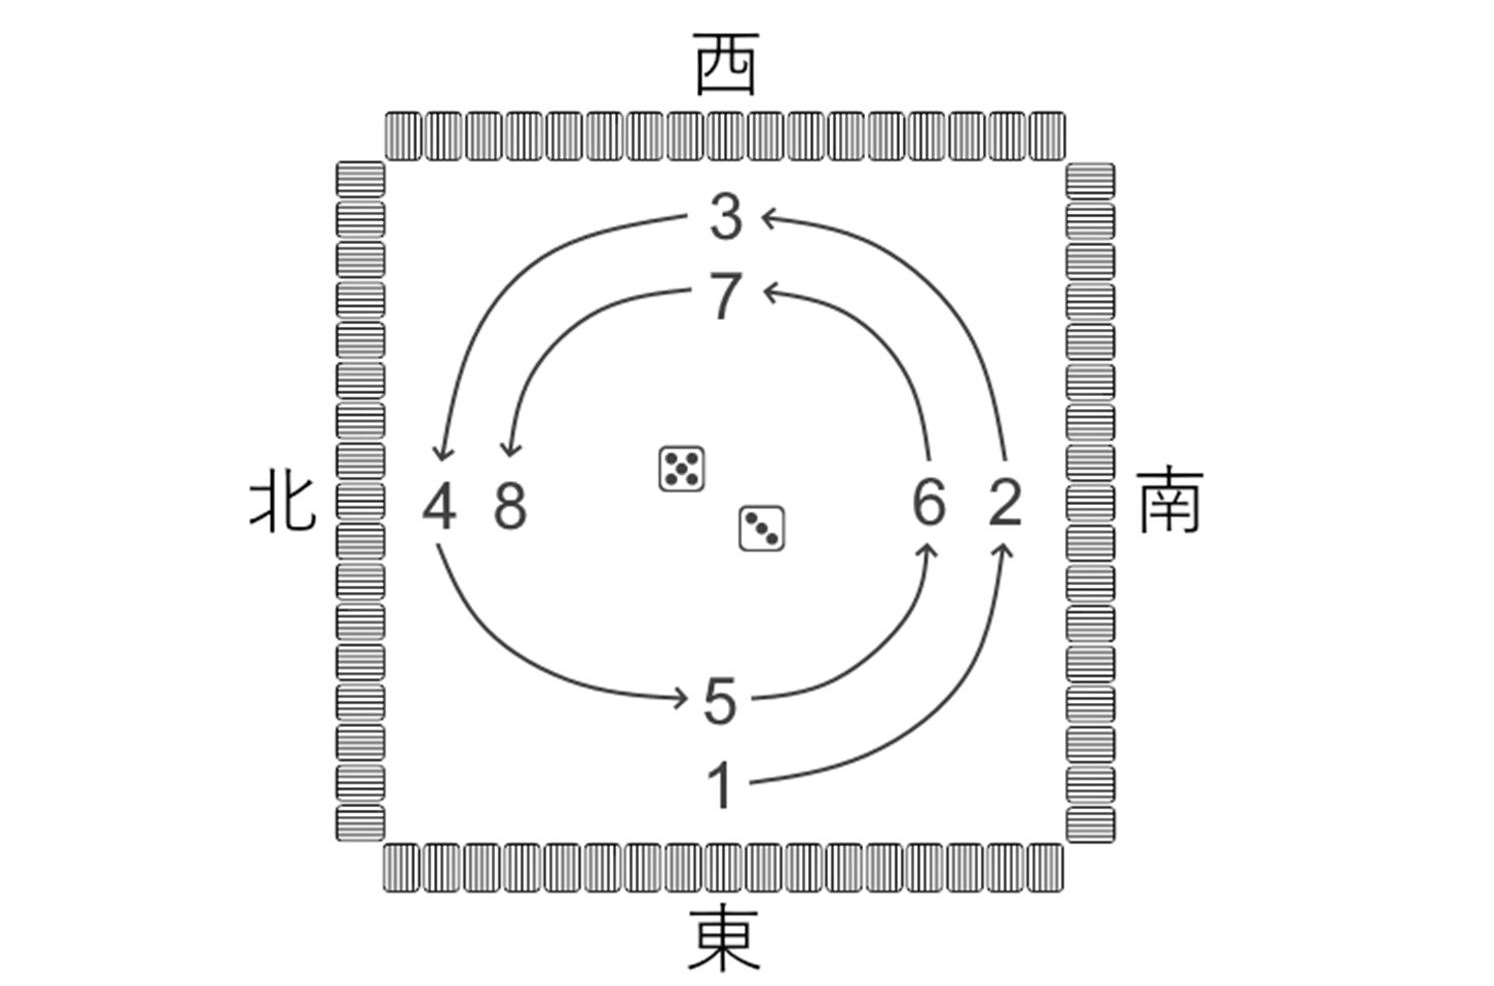
\includegraphics[width=16cm]{table-deal-start.png}
	\caption{Определение разлома стены}
\end{figure}

Затем игрок, на чью сторону указал дилер (в примере выше – север) отсчитывает от правого конца своей стороны стены столько тайлов, какое число выпало на кубиках до этого (в примере – 8) и немного отодвигает их от соседних тайлов вправо, создавая разлом стены. После этого он отсчитывает от разлома в обратную сторону 7 тайлов и делает второй разлом, обособляя получившуюся группу из 14 тайлов (см. рис.2). Эта группа называется мёртвой стеной и не разбирается в процессе игры. Оставшаяся часть стены называется живой стеной и используется во время раздачи для получения игроками тайлов (наподобие колоды карт). Разбирается она стопками верхний-нижний по часовой стрелке, начиная с верхнего тайла первой стопки после разлома и заканчивая нижним последней перед мёртвой стеной. Стена считается непрерывной, и переход через углы не имеет никакого значения как при формировании мёртвой стены, так и при последующем разборе.

Третий верхний тайл от конца мёртвой стены переворачивается рубашкой вниз (на рисунке это 6 ман) и служит в данной раздаче индикатором доры – тайла, дающего дополнительные очки при его наличии в руке. Подробно о дорах и принципе работы индикаторов рассказано в разделе VIII.

\begin{figure}[H]
	\centering
	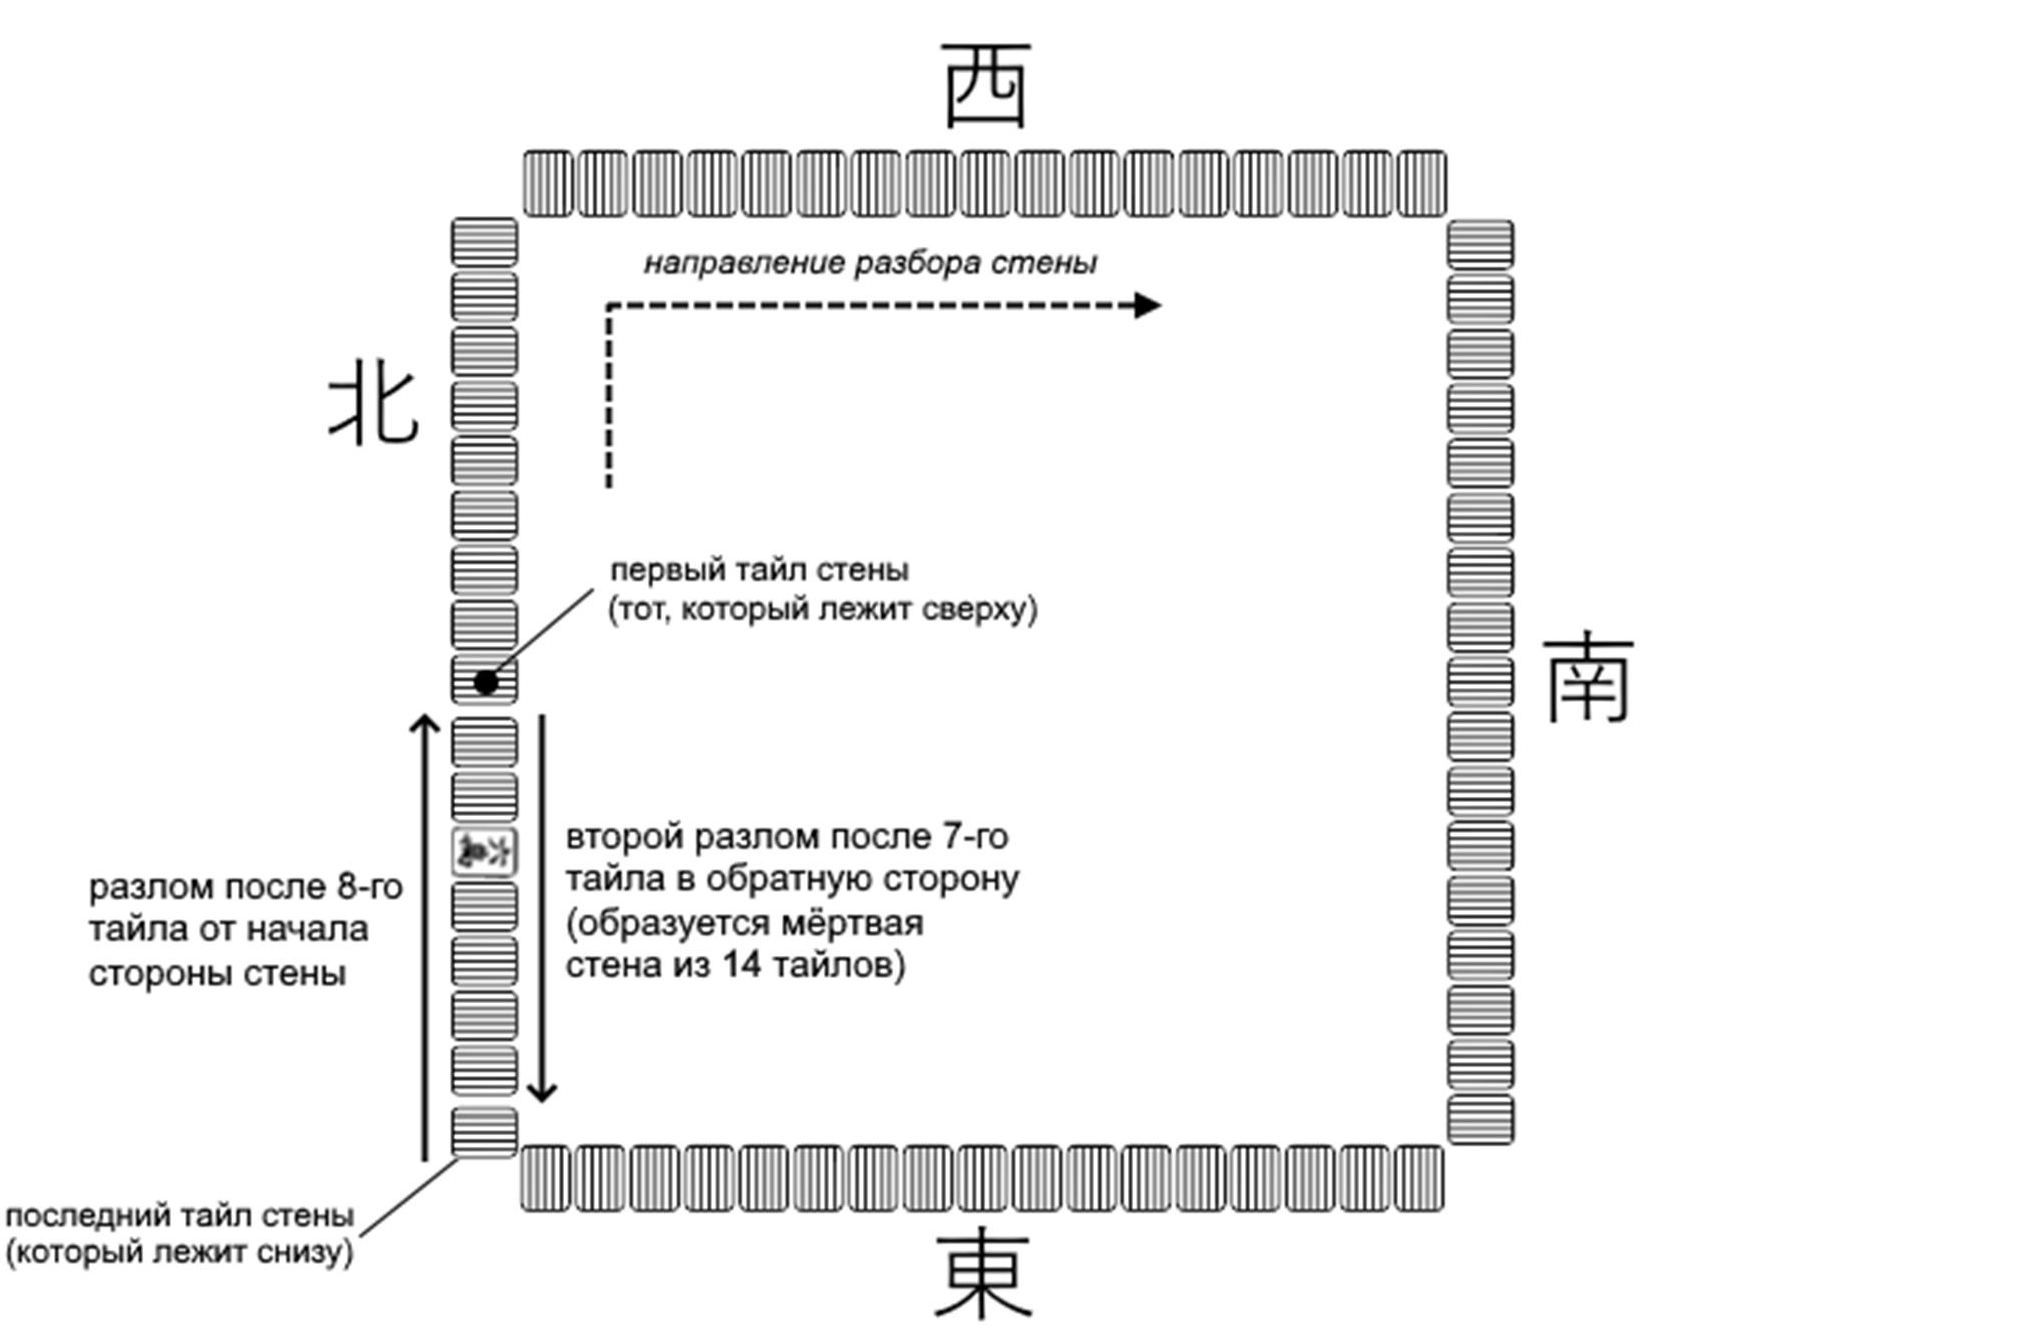
\includegraphics[width=16cm]{table-deal-start-2.png}
	\caption{Мертвая и живая стены}
\end{figure}

После открытия индикатора доры игроки берут себе со стены тайлы в стартовые руки. Начиная с дилера по очереди против часовой стрелки игроки начинают брать от начала живой стены по четыре тайла (две стопки по 2), пока у каждого не окажется 12 тайлов. После этого игроки в том же порядке берут ещё по одному тайлу (порядок разбора – всегда от верхнего к нижнему), а затем дилер берёт себе ещё один тайл (см. рис.3). Таким образом, в начале раздачи дилер имеет 14 тайлов, а остальные – по 13. Тайлы своих рук игроки расставляют перед собой в ряд вертикально изображением к себе, так, чтобы остальные видели только их рубашки. Для удобства игроки сортируют руки: ставят рядом тайлы одной масти по порядку номеров и одинаковые благородные тайлы. Допустим, игрок взял себе в стартовую руку следующие тайлы:

\mahjong{5m 6s 4m 8s 3z 9m 7z 2z 1s 3m 7z 7s 4m}

Он может отсортировать их следующим образом:

\mahjong{1s 678s 34459m 2377z}

Разные масти могут быть отсортированы слева направо или справа налево, а разные благородные тайлы могут стоять в разных местах – всё зависит от удобства для игрока и времени, затрачиваемого на сортировку.

В компьютерном маджонге построение стены, её разлом, набор и сортировка стартовых рук как правило происходят автоматически, и когда начинается раздача игроки сразу же видят свои отсортированные стартовые руки и индикатор доры. 

\begin{figure}[H]
	\centering
	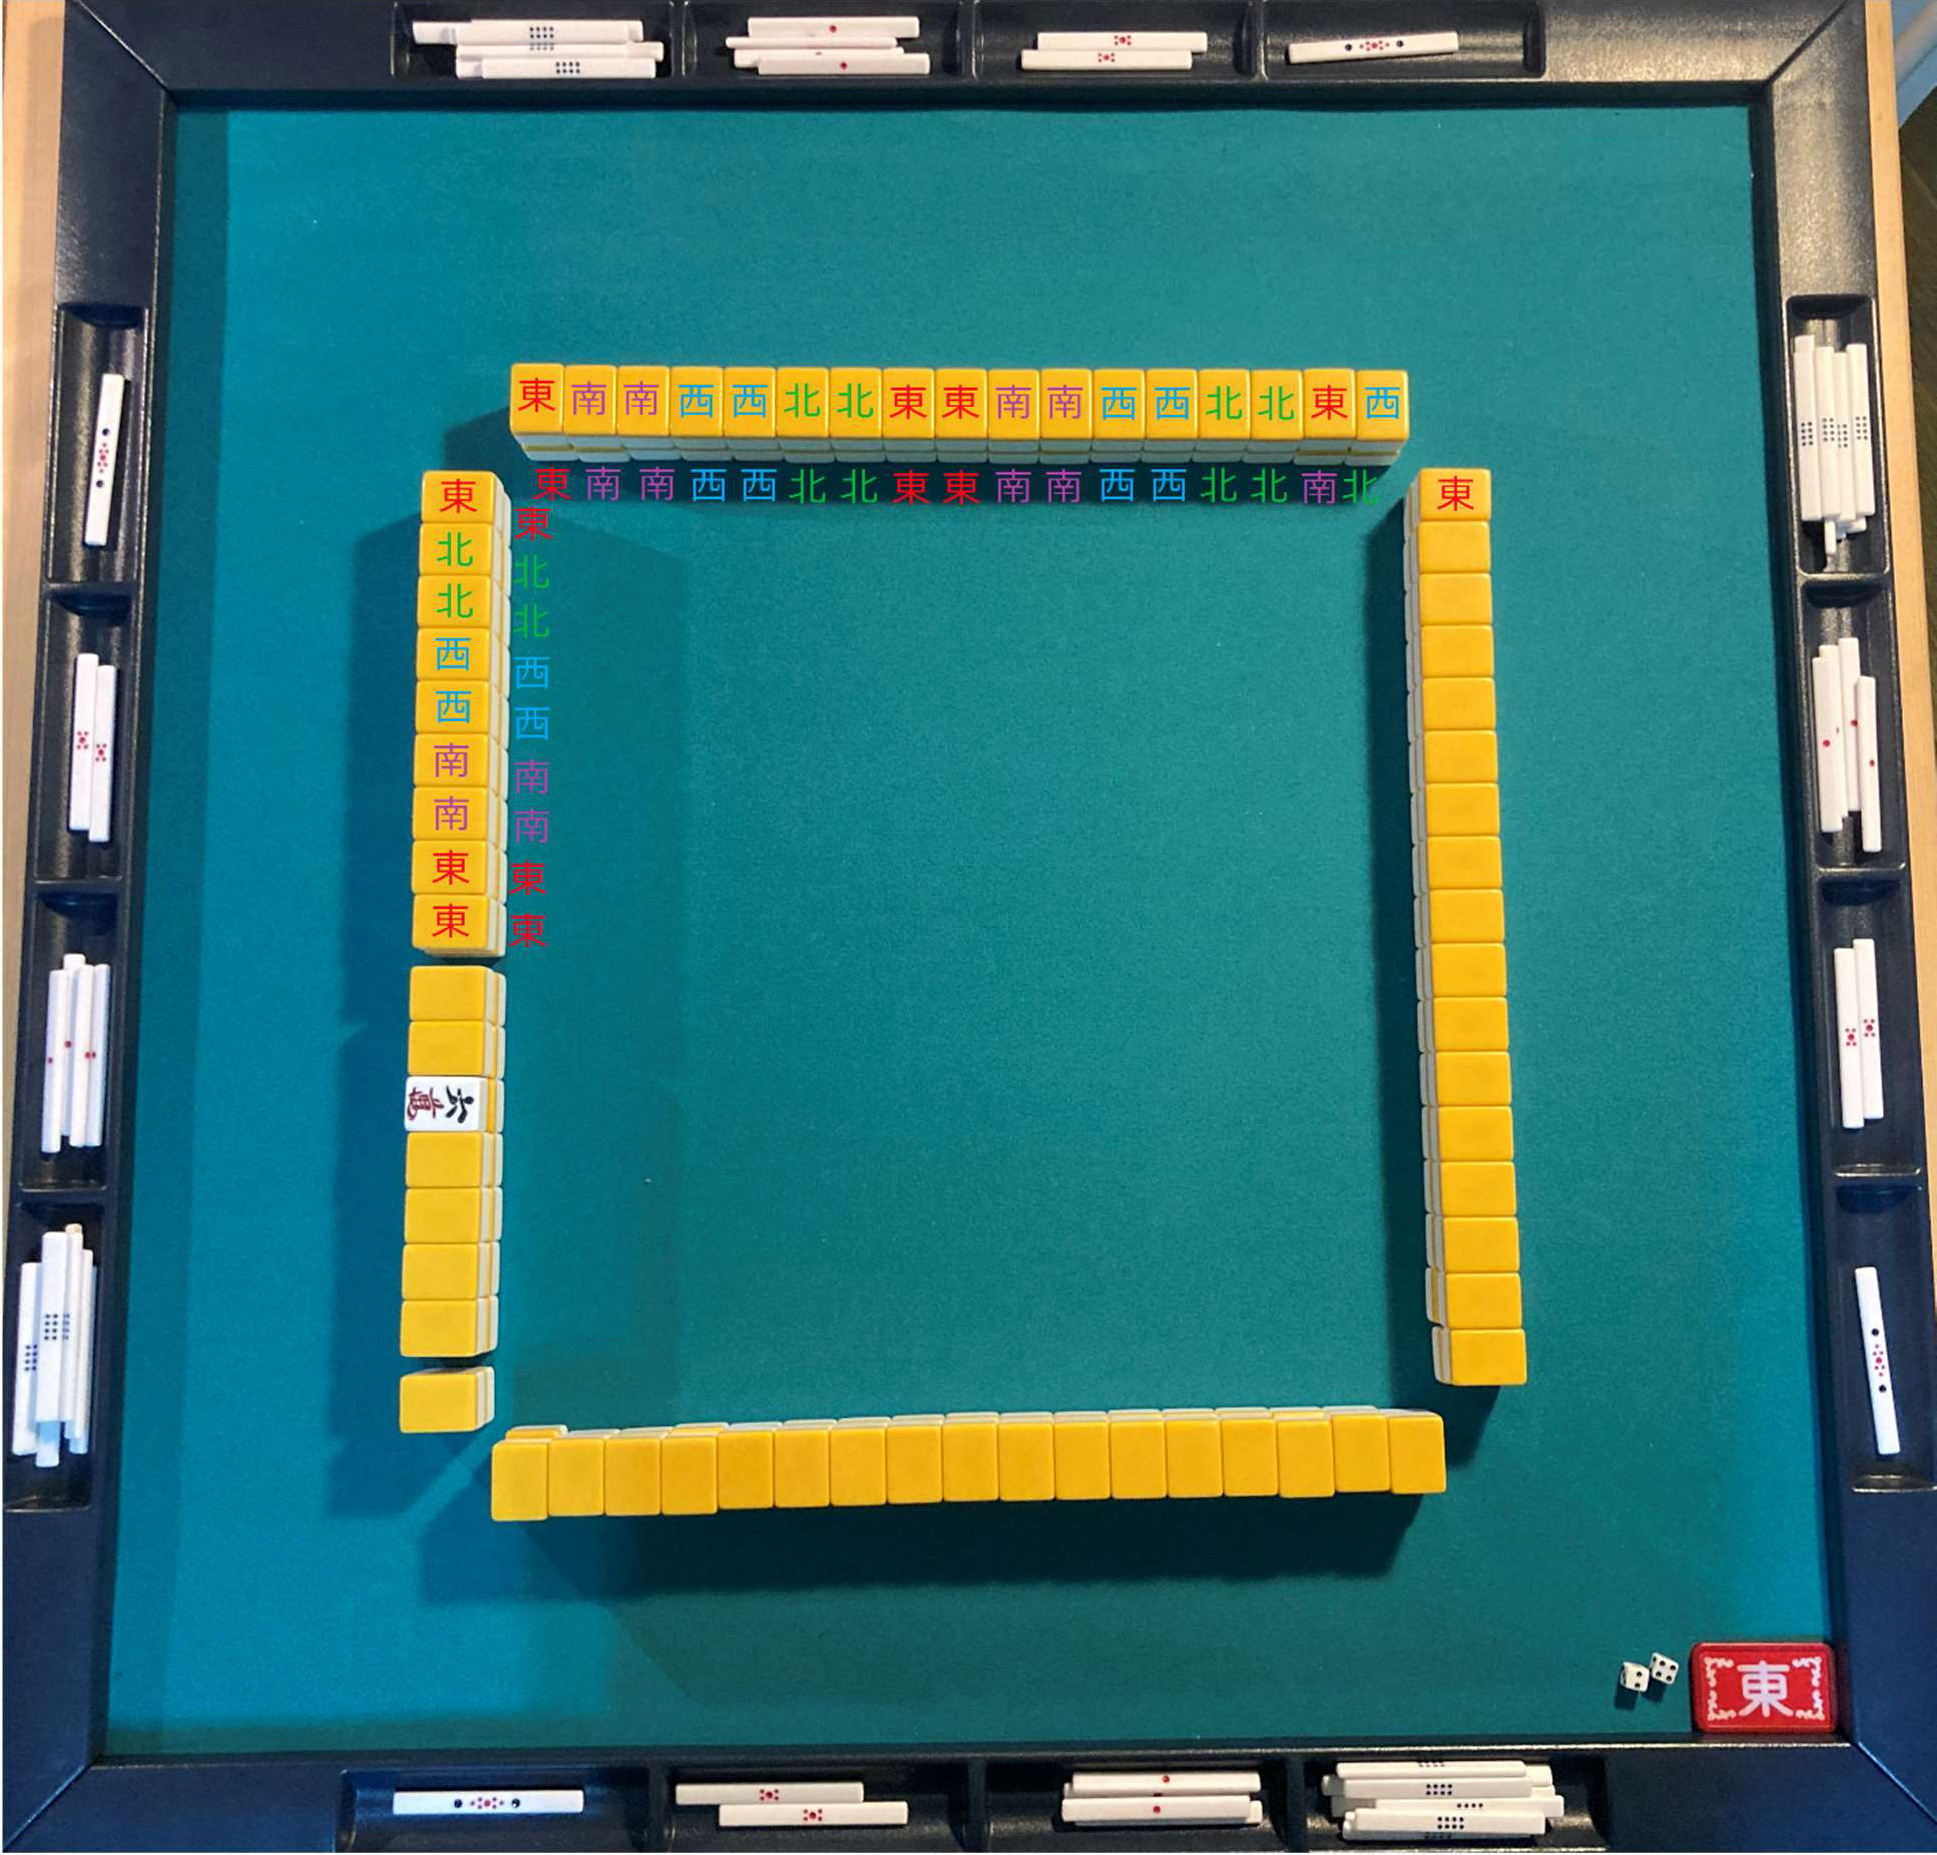
\includegraphics[width=16cm]{table-deal-start-3.png}
	\caption{Порядок разбора стены, фото}
\end{figure}

Обратите внимание на подписи тайлов - они показывают, какой игрок должен их взять (верхние тайлы стены подписаны прямо на рубашке, нижние – рядом). Предположим, что сейчас идёт первая раздача восточного раунда: индикатор первого дилера повёрнут иероглифом востока кверху, а кубики как индикатор текущего дилера лежат рядом с ним, т. е. первый дилер является дилером в этой раздаче.

\subsection{Ход раздачи}

В ходе раздачи, которая начинается сразу же после набора и сортировки всеми стартовых рук, игроки изменяют состав своих рук, набирая в них по одному новые тайлы с живой стены и выбрасывая ненужные. Цель каждого игрока в раздаче – собрать в руке четыре сета и одну пару (два одинаковых тайла). При объявлении кем-либо победы с готовой рукой раздача заканчивается. Цель всей игры – набрать как можно больше очков, получаемых в основном за собранные руки.

Сет – это определённая комбинация из трёх или четырёх тайлов. Они бывают трёх видов:
\begin{itemize}
	\item Три одинаковых тайла - \textit{пон};
	\item Четыре одинаковых тайла – \textit{кан};
	\item Последовательность из трёх тайлов одной масти подряд (по типу 1-2-3, 3-4-5 и т. п.) – \textit{чи}. Последовательности можно собирать только из тайлов мастей, и в них не должно быть перехода через девятку: 8-9-1 и 9-1-2 не засчитываются как чи.
\end{itemize}

Один тайл не может одновременно входить в два сета. В примере ниже в руке уже есть готовый пон из 4 ман, чи 7-8-9 ман и пара красных драконов, но последовательность 3-4-5-6-7 пин не засчитывается за два чи: для завершения этой формы в два сета требуется получить ещё один тайл (2, 5 либо 8 пин).

\mahjong{444789m 34567p 77z}

В руке из примера выше 13 тайлов, как и в любой руке не-дилера в начале раздачи, но выигрышная рука должна содержать как минимум 14 тайлов (3+3+3+3+2, если же в руке есть каны, число тайлов может доходить до 18). Четырнадцатый тайл игроки получают в свои ходы во время раздачи: раздача начинается с хода дилера, который сбрасывает из руки один из своих 14 тайлов, кладя его рубашкой вниз в центр стола; затем ход переходит к следующему игроку против часовой стрелки, который берёт первый тайл из оставшейся части живой стены и также сбрасывает один тайл из своей руки (можно сбрасывать и тайл, только что взятый со стены – такой сброс называется \textit{цумогири}). Затем ход переходит к следующему игроку, и так раздача продолжается до тех пор, пока кто-либо не соберёт руку и объявит победу, или же пока в живой стене не закончатся тайлы. 

Ходы в риичи-маджонге обязательны, пропускать взятие со стены либо сброс нельзя. Каны, а вместе с ними и руки, содержащие более 14 тайлов, возможно образовать специальными объявлениями, о которых рассказывается в следующем разделе. Ходы четырёх игроков, начиная от дилера, образуют круг раздачи. После окончания круга ход вновь переходит к дилеру, и начинается следующий круг. Группы сброшенных тайлов в центре стола называются сбросами или \textit{дискардами}. Каждый игрок имеет свой отдельный дискард. Тайлы следует выкладывать в сброс слева направо тремя рядами по 6 штук (начиная с ближнего к центру стола и далее по направлению к себе); четвёртый же ряд чаще не начинают, а вместо этого продолжают третий.

\begin{figure}[H]
	\centering
	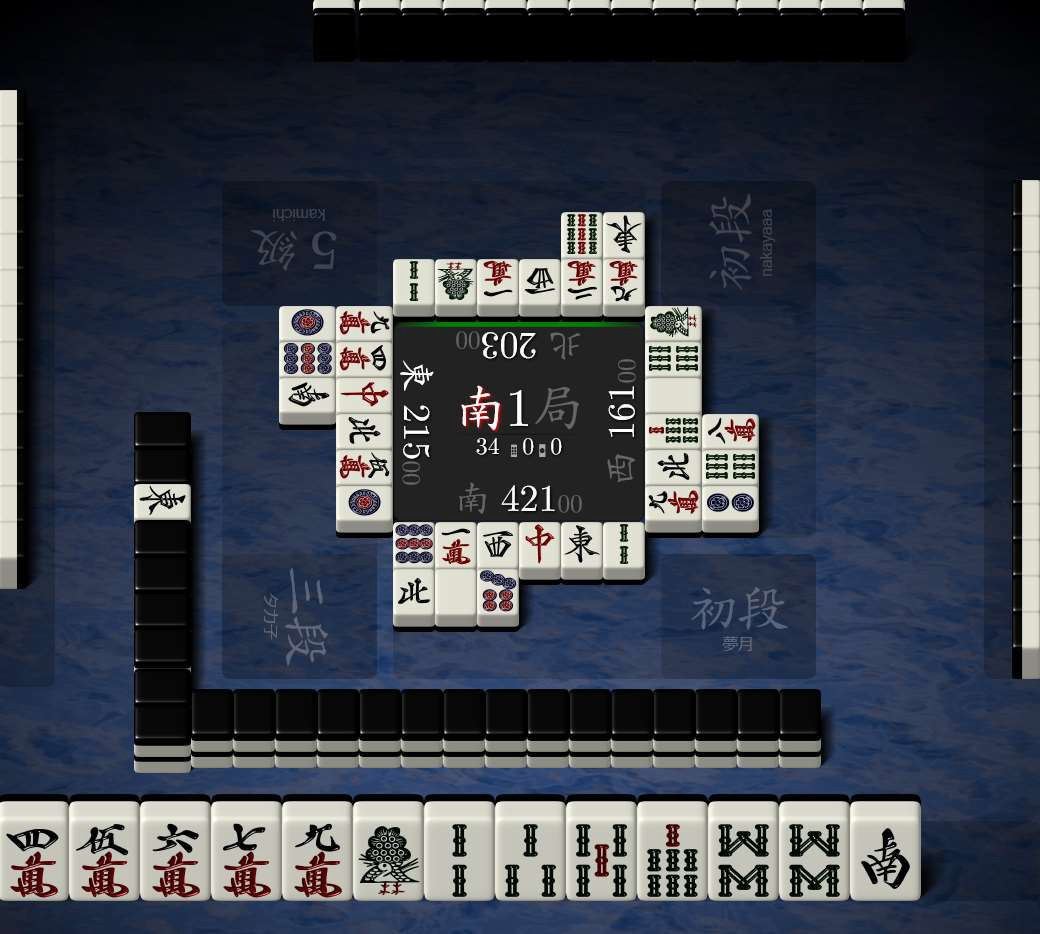
\includegraphics[width=16cm]{tenhou-deal.jpg}
	\caption{Пример раздачи на сервере tenhou.net}
\end{figure}

Рассмотрим вид стола в процессе раздачи на онлайн-сервере tenhou.net (рис.4). В центре – указатель раунда и номера раздачи за раунд (южный, первая) и указатели мест игроков со счётчиками очков (мы юг с 42100 очков; на онлайн-серверах вместо палочек используются цифровые счётчики). Вокруг центра – дискарды игроков, ниже – живая стена, слева – мёртвая стена с индикатором доры восточным ветром. По краям стола расположены руки игроков. Сейчас 9-й круг, ход севера: он получил тайл со стены, но ещё не совершил сброс. Пришедший со стены тайл сначала ставят отдельно (здесь он стоит слева от основной руки, если смотреть от нас), и встраивают в руку только после сброса, если сброшен другой тайл.

\subsection{Объявления в игре}

% TODO: Сорокин

Раздел в работе. Проверить, что следующие моменты описаны в разделе при его добавлении:

Риичи: единственное объявление, которое не прерывает круг. Важное уточнение для последующих объяснений.

Кан при риичи: не может менять интерпретацию руки (но может менять список яку, например, игрок может получить санканцу сверху).

Дабл-рон и трипл-рон: есть. 

Невыигравшие палки при даблроне: отдаются первому по ходу раздачи победившему. Выигравшие палки возвращаются объявившим.

Хонба при даблроне платится всем победителям в полном объеме.

При даблроне/триплроне невалидный рон наказывается вежливым указанием, при повторе может быть назначен штраф.

Куикаэ: не допускается ни в каком виде

\subsection{Фуритен и временный фуритен}

Правило \textit{фуритен} (\textnihon{フリテン}), или правило упущенного сброса, запрещает игроку объявлять рон, если хоть один из выигрышных тайлов, завершающих руку, лежит у него в дискарде. При этом как дискард учитываются и тайлы, взятые оттуда для сетов другими игроками. Именно из-за этого при объявлениях сетов требуется указывать какой тайл был взят и с кого из противников, кладя один из тайлов боком с соответствующей стороны.

Например, рассмотрим игрока со следующей рукой:

\mahjong{33456678m 23p 678s}

Предположим, дискард у игрока следующий:

\mahjong{1p 4z 7z 2s 4s 9m}

В данном случае игрок не может объявить рон ни при сбросе противником 1 пин, ни при сбросе 4 пин, потому что в его дискарде есть «упущенный» выигрышный тайл 1 пин. При этом ограничений на объявление цумо нет. Если игрок перестроит свою руку так, чтобы сброшенные в дискард тайлы не завершали выигрышное ожидание, фуритен перестанет действовать, и он снова сможет объявлять рон. Например, это будет возможно если руку выше изменить следующим образом взятием 5 пин и сбросом 2 пин: 

\mahjong{33456678m 35p 678s}

В этом случае ожидание на 1 пин пропадёт, и игрок сможет объявить рон на сброшенную кем-либо 4 пин. 

Фуритен даёт возможность для игры в защиту: тайлы, лежащие в сбросе у противника, можно уверенно сбрасывать, не опасаясь, что он объявит на них рон (при победе по рону игрок получает очки за счёт сбросившего выигрышный тайл; о выплатах см. раздел IX). Есть и более продвинутые приёмы защиты, основанные на фуритене, которым посвящены отдельные специализированные статьи, в данном руководстве не рассматриваемые.

\textit{Временный фуритен} – это отдельное правило, которое не позволяет игроку объявлять рон, если на текущем круге считая от хода игрока уже был сброшен какой-либо из выигрышных для него тайлов. Действие временного фуритена заканчивается с первым же ходом игрока – в момент, когда игрок формально может сменить ожидание. Допустим у нас на нашем ходу имеется следующая рука:

\mahjong{123456789m 99s 11z}

В случае если игрок справа сбросил 9 со и мы пропустили возможный рон, а сразу за ним игрок напротив сбрасывает восток или ещё одну 9 со, объявлять рон на этот тайл нельзя, потому что на этом круге рон уже был пропущен. Если же кто-то ещё раз сбросит 9 со или восток уже после следующего нашего хода, рон объявить будет можно.

Временный фуритен существует для предотвращения избирательности в объявлении рона, но иногда действует во вред игрокам в темпае, если после одного пропущенного выигрышного тайла на том же круге сбрасывается тайл, дающий руке большую стоимость, чем первый. Если игрок пропустил один рон после объявления риичи, из-за временного фуритена он не может победить по рону до конца раздачи, т. к. после риичи сменить ожидание невозможно (подробно о риичи рассказывается в посвящённом ему разделе VII).

\subsection{Яку: условия победы}

Для объявления победы необходимы не только четыре сета и пара в руке, но и выполнение хотя бы одного \textit{яку} – условия победы, приносящего руке стоимость. Рука без яку не имеет стоимости, и \lineunder{с такой рукой объявлять победу нельзя}, даже если собраны все сеты и пара. Яку бывают двух типов: это либо наличие определённых комбинаций тайлов в руке, либо особые игровые ситуации, при которых происходит победа. Стоимость яку измерима: каждое из них имеет фиксированную стоимость в \textit{ханах} (яп. \textnihon{飜} или \textnihon{翻}) – специальных единицах, используемых для удобства, которые при подсчёте общей стоимости руки переводятся в очки.

Яку бывают \textbf{комбинационными} и \textbf{ситуационными}. 

Комбинационные яку даются за сочетания тайлов в руке, объединенные некоторым общим принципом. Яку может давать как часть руки (например, в случае комбинации \textit{якухай} яку дается за любой пон драконов или ветров места или раунда), так и вся рука полностью - в случае выполнения некоторого условия для всей руки без исключения (например, яку \textit{тойтой} дается в случае если вся рука состоит только из понов). 

Ситуационные яку даются за выполнение некоторых игровых условий, не связанных с формой руки (например, \textit{риншан кайхо} дается за победу с замещающего тайла при объявлении кана).

Полный список яку с подробным описанием приведен в приложении.

Яку можно сочетать друг с другом – в таких случаях стоимости всех яку в руке суммируются (за некоторыми исключениями; все исключения описаны в приложении).

Некоторые яку невозможно сочетать, потому что их условия противоречат друг другу. Например, \textit{чанта} не сочетается с \textit{тан'яо}, потому что требует наличия крайних или благородных тайлов, которых в руке с тан'яо быть не может. В других случаях теоретически возможные сочетания яку запрещены правилами.

Некоторые яку требуют специфических ожиданий - в этом случае при победе игрокам запрещается встраивать выигрышный тайл в руку – иначе другие игроки после открытия руки не смогут его проверить.

\subsubsection{Якуманы}

Некоторые яку, называемые \textit{якуманами}, собираются настолько редко и тяжело, что стоят максимально возможное количество очков (32000 очков для не-дилера и в 48000 для дилера). Якуманы не сочетаются ни с какими яку, кроме других якуманов – именно поэтому их стоимость обычно считают сразу в очках, хотя можно записать её и в ханах – 13. Когда в руке несколько якуманов, они складываются, образуя двойные, тройные якуманы и т. д., а стоимость руки с каждым дополнительным якуманом возрастает ещё на 32000 / 48000 очков. Якуманы также бывают как комбинационными, так и ситуационными - полный список с описаниями можно найти в приложении.

\subsection{Дора}

Дора (\textnihon{ドラ}) – это тайл, наличие которого в руке увеличивает её стоимость на 1 хан. Однако дора не даёт яку, и с рукой без яку нельзя объявить победу даже если в ней есть доры. Дора в каждой раздаче определяется индикатором, который открывается в мёртвой стене перед её началом. Дорой считается следующий тайл после индикатора по порядку, указанному в разделе о наборе тайлов:
\begin{itemize}
	\item Тайлы мастей: 1→2→3→4→5→6→7→8→9→1 (дора только в той же масти, что и индикатор);
	\item Ветра: \textnihon{東}→\textnihon{南}→\textnihon{西}→\textnihon{北}→\textnihon{東};
	\item Драконы: красный→белый→зелёный→красный.
\end{itemize}

Например, если индикатор – 2 пин, дорой является 3 пин; если индикатор 9 соу, дора – 1 соу; если красный дракон, то дорой будет белый.
Когда в руке есть несколько экземпляров дор, их стоимость складывается:

\mahjong{233445m 567p 4599s-3s}

Мертвая стена:
\mahjong{XX3mXXXX}

Эта рука без ситуационных яку будет стоить 3 хан: один за пинфу и ещё по одному за две доры 4 ман.

Помимо «обычных» дор существуют дополнительные, многие из которых ранее уже упоминались. За каждый экземпляр любой из них даётся дополнительный хан, как и за обычную дору:
\begin{itemize}
	\item \textit{Кандоры}. При объявлении любого кана в мёртвой стене открывается один индикатор кандоры (соседний тайл с индикатором доры с той стороны, где от него до конца стены 4 тайла). Всего их может быть открыто 4, по числу тайлов от индикатора доры до конца мёртвой стены (пятый кан за раздачу объявлять запрещено). Сколько в раздаче объявлено канов, столько и открыто индикаторов кандор. Индикаторы работают точно так же, как и обычные.
	\item \textit{Урадоры}. При победе после объявления риичи, тайл, находящийся в мёртвой стене под индикатором доры, открывается и становится дополнительным индикатором доры, которая называется урадорой. Если в выигранной руке риичи-игрока оказываются урадоры, он получает за них дополнительную стоимость. Индикаторы открывает лично выигравший руку с риичи игрок либо игрок, со стороны которого находится мёртвая стена.
	\item \textit{Кан-урадоры}. Если во время раздачи объявлялись каны, при победе после риичи открывается и становится индикатором не только тайл под индикатором доры, но и все тайлы под открытыми индикаторами кандор. Например, если за раздачу было объявлено два кана, урадор будет три: одна обычная и две кан-урадоры.
\end{itemize}

Таким образом, все тайлы мёртвой стены, кроме добавляемых в неё из живой стены после объявления канов, теоретически могут быть использованы в игре либо как тайлы замены, либо как индикаторы дор (см. схему мёртвой стены в разделе IV).

Также в данных правилах регламентируются \textit{акадоры}: рисунок на некоторых экземплярах пятёрок мастей сделан полностью красным, и каждая такая пятёрка в руке увеличивает её стоимость на 1 хан. Акадор в наборах три, по одной в каждой масти. Использование акадор в наборах является обязательным, если иное не указано в сопутствующем регламенте конкретного турнира из-за обстоятельств непреодолимой силы (например, в случае, если у организаторов недостаточно наборов с акадорами).

Если несколько одинаковых индикаторов доры указывают на один и тот же тайл, он становится двойной, тройной или четверной дорой по числу указывающих индикаторов, и такие доры дают соответственно 2, 3 или 4 дополнительных хана за каждый тайл. Если индикатор указывает на пятёрку, стоимость акадоры также увеличивается на 1 хан:

\mahjong{788m24056p246s22z}

Мертвая стена:
\mahjong{XX1z4p1zXX}

Эта рука содержит дор на 7 хан.

\subsection{Подсчёт стоимости руки и порядок выплат}

Стоимость руки сначала считается как сумма всех ханов, полученных за яку и доры, и всех фу (\textnihon{符}) – «мини-очков», начисляемых за определённые сеты в руке, форму ожидания на выигрышный тайл и другие мелкие особенности руки, не дающие яку. После этого стоимость, выраженная в ханах и фу (например, 2 хан 40 фу), переводится в очки по специальной таблице или формуле, которые будут рассмотрены далее.

Мини-очки \textit{фу} поощряют игрока за мелкие сложности в сборе руки, не дающие новых яку. Они считаются после подсчёта суммарного количества ханов за яку и доры. Если в руке 5 хан или больше, фу считать не нужно: стоимость такой руки в очках будет зависеть только от количества ханов.
Фу начисляются за поны и каны в руке, якухайные пары, ожидание на выигрышный тайл и тип победы. Каждая рука, если она стоит менее 5 хан, по умолчанию имеет 20 фу, и все остальные полученные фу складываются с ними. После подсчёта всех фу получившееся число округляется вверх до десятков (например, если при суммировании получилось 54 фу, итоговым значением будет 60). Единственное исключение – читойцу: любая рука из семи пар (опять же, если её общая стоимость – менее 5 хан) оценивается в 25 фу, никакие дополнительные фу к ним не прибавляются, и это число не округляется вверх до 30.

\subsubsection{Фу за поны и каны}

Количество фу зависит от открытости сетов (не всей руки!) и тайлов, из которых они состоят:

\begin{tabular}{|L{7cm}|C{3cm}|C{3cm}|}
	\hline
	& Открытый сет &
	Закрытый сет \\
	\hline
	Пон средних тайлов &
	+ 2 фу &
	+ 4 фу \\
	\hline
	Пон крайних или благородных тайлов &
	+ 4 фу &
	+ 8 фу \\
	\hline
	Кан средних тайлов &
	+ 8 фу &
	+ 16 фу \\
	\hline
	Кан крайних или благородных тайлов &
	+ 16 фу &
	+ 32 фу \\
	\hline
\end{tabular}

Фу начисляются за каждый отдельный пон и кан в руке в зависимости от его типа по таблице. Если пон образовался в руке с получением выигрышного тайла, он считается открытым, если тайл получен по рону, и закрытым, если по цумо. За чи, как более простые в сборе сеты, фу не даётся.

\subsubsection{Фу за якухайные пары}

Если в руке пара состоит из тайлов, сет которых дал бы якухай (драконы или ветра раунда/места), за такую пару начисляется 2 дополнительных фу. За пару совпадающих ветров раунда и места, сет которых дал бы двойной якухай, обычно даётся 4 фу. Всё это не относится к читойцу: такие руки всегда стоят 25 фу.

\subsubsection{Фу за тип победы}

\begin{itemize}
	\item При победе по рону с закрытой рукой даётся 10 дополнительных фу;
	\item При победе по цумо с любой рукой (открытой или закрытой) даётся 2 дополнительных фу, если эта рука не содержит пинфу\footnote{Можно заметить, что все условия для пинфу подобраны так, чтобы рука в итоге не получила фу кроме базовых 20: в ней нет ни коцу и канов, ни якухайных пар, ни ценных ожиданий. Действительно, буквальный перевод названия "пинфу" – это «рука без фу». Единственное исключение – +10 фу за рон на закрытой руке.}. При победе с тайла замены (риншан кайхо) 2 фу за цумо тоже не начисляются;
	\item При победе по рону с открытой рукой, в которой выполняются все остальные условия для пинфу (нет понов, канов и якухайных пар, ожидание в две стороны в рянмен) даётся 2 дополнительных фу. Других фу, кроме базовых, в такой руке нет, и поэтому она всегда стоит 30 фу.
\end{itemize}

\subsubsection{Фу за ожидание на выигрышный тайл}

В темпае возможны пять различных базовых форм ожидания выигрышного тайла, и некоторые, наиболее «неудобные» из них, оцениваются в дополнительные 2 фу:

\noindent\begin{tabular}{|C{3cm}|C{5cm}|C{3cm}|C{3cm}|}
\hline
	Название  &
	Пример формы &
	Выигрышные тайлы &
	Фу \\
\hline
	\rule[0ex]{0pt}{5ex} Рянмен \newline (в две стороны) \newline &
	\mahjong{34p} &
	\mahjong{25p} &
	не начисляется \\
\hline
	\rule[0ex]{0pt}{5ex} Канчан \newline (в «дырку») \newline &
	\mahjong{35s} &
	\mahjong{4s} &
	+2 фу \\
\hline
	\rule[0ex]{0pt}{5ex} Пенчан \newline (краевое) \newline &
	\mahjong{12m} &
	\mahjong{3m} &
	+2 фу \\
\hline
	\rule[0ex]{0pt}{5ex} Танки \newline (в пару) \newline &
	\mahjong{3s} &
	\mahjong{3s} &
	+2 фу \\
\hline
	\rule[0ex]{0pt}{5ex} Сянпон \newline (в две пары) \newline &
	\mahjong{33z-11m} &
	\mahjong{3z1m} &
	не начисляется \\
\hline
\end{tabular}

За сянпон как ожидание фу не даётся, но 2, 4 или 8 фу начисляется за получившийся пон в соответствии с таблицей фу за сеты. Если выигрышный тайл пришёл одновременно в несколько ожиданий разного типа, считается только то, с которым рука получается дороже всего в очках (о пересчёте ханов и фу в очки см. следующий раздел) – это же касается и интерпретации сетов в руке. Например, если считать в руке ниже выигрышным ожиданием рянмен 5-6, а не пенчан 8-9, она получит дополнительный хан за  пинфу,  и поэтому будет выбрана такая интерпретация ожиданий. Соответственно, 2 фу за пенчан начислены не будут.

\mahjong{23466m 56789p 123s-7p}

В случае более сложных ожиданий, эти ожидания всегда можно свести к базовым и рассчитать соответствующую стоимость. Например, формы \textit{нобетан} и \textit{санментан} всегда ждут только в пару (пусть и несколько разновидностей тайлов), тогда как форма \textit{рянтан} может рассматриваться как рянмен и как танки (отсюда и название формы). Рассмотрим примеры таких форм.

\textbf{Нобетан}

\mahjong{3456p}

Эту форму можно рассмотреть как чи + ожидание в пару двумя способами:

\mahjong{3p-456p}

\mahjong{345p-6p}

\textbf{Санментан}

\mahjong{3456789s}

Тут аналогично, но способов уже три:

\mahjong {3s-456s-789s}

\mahjong{345s-6s-789s}

\mahjong{345s-678s-9s}

\textbf{Рянтан}

\mahjong{3444m}

Эту форму можно рассмотреть либо как пон + ожидание в пару, либо как пару + ожидание в две стороны:

\mahjong{3m-444m} 

\mahjong{34m-44m}

Существуют и другие комплексные формы ожиданий, но каждую из них можно разложить до базовых форм тем или иным способом.

\subsubsection{Примеры подсчёта ханов и фу в руке}

Пример №1.

\mahjong{123m99p13s-2s}\hfill \mahjong{8'79s 66'6z}

Мертвая стена:
\mahjong{XX9mXXXX}

(раунд южный, игрок на востоке, победа без ситуационных яку)

\begin{tabular}{lr}
	Якухай & 1 хан \\
	Открытая чанта & 1 хан \\
	Доры & 1 хан \\
	Базовые фу & 20 фу \\
	Открытый пон благородных тайлов & 4 фу \\
	Ожидание в канчан & 2 фу \\
	\hline
	\textbf{Итого} & \textbf{3 хан 30 фу} \\
\end{tabular}

Пример №2.

\mahjong{340567m 44s 22z-4s} \hfill \mahjong{X99mX}

Мертвая стена: \mahjong{XX2p3zXXX}

Нижний ряд мертвой стены: \mahjong{XX6m9pXXX}

(раунд восточный, игрок на юге, победа по риичи без иппацу и других ситуационных яку с другого игрока)

\begin{tabular}{lr}
	Риичи & 1 хан \\
	Акадора & 1 хан \\
	Урадора & 1 хан \\
	Базовые фу & 20 фу \\
	Закрытый кан крайних тайлов & 32 фу \\
	Открытый пон средних тайлов (4 соу) & 2 фу \\
	Якухайная пара & 2 фу \\
	Закрытый рон & 10 фу \\
	\hline
	\textbf{Итого} & \textbf{3 хан 70 фу} \\
\end{tabular}

Пример №3. 

\mahjong{455667p3z-3z}

Мертвая стена: \mahjong{XX3p4s3pXX}

(раунд южный, игрок на севере, победа с тайла замены)

\begin{tabular}{lr}
	Якухай & 1 хан \\
	Открытое хон'ицу & 2 хан \\
	Риншан кайхо & 1 хан \\
	Доры & 2 хан \\
	\multicolumn{2}{l}{В руке больше 4 хан, фу не подсчитываются} \\
	\hline
	\textbf{Итого} & \textbf{6 хан} \\
\end{tabular}

Пример №4.

\mahjong{5688m 456p 678s-4m} \hfill \mahjong{4'23p}

Мертвая стена: \mahjong{XX6mXXXX}

(раунд восточный, игрок на востоке, победа без ситуационных яку)

\begin{tabular}{lr}
	Тан'яо & 1 хан \\
	Базовые фу & 20 фу \\
	Рон с «открытым пинфу» & 2 фу \\
	\hline
	\textbf{Итого} & \textbf{1 хан 30 фу} \\
\end{tabular}

Пример №5.

\mahjong{222m 678p 1406888s-1s}

Мертвая стена: \mahjong{XX4zXXXX}

(раунд южный, игрок на западе, победа с закрытым цумо без других ситуационных яку)

\begin{tabular}{lr}
	Мензен цумо & 1 хан \\
	Акадора & 1 хан \\
	Базовые фу & 20 фу \\
	Два закрытых пона средних тайлов & 8 фу \\
	Ожидание в танки (в пару) & 2 фу \\
	Цумо & 2 фу \\
	\hline
	\textbf{Итого} & \textbf{2 хан 40 фу} \\
\end{tabular}

\subsubsection{Подсчет очков в руке}

В риичи-маджонге все игроки начинают игру с 30000 очков, и в процессе игры только обмениваются очками друг с другом: больше очки ниоткуда не появляются и никуда не исчезают. Поэтому сумма очков за столом всегда равна 120000.

Выплаты за собранные руки производятся сразу после объявления победы и подсчёта очков, перед началом следующей раздачи. После рона всю стоимость руки победителю выплачивает игрок, сбросивший выигрышный тайл, а при цумо выплата делится между всеми тремя оставшимися игроками. При двойном или тройном роне набросивший игрок платит всем победителям.

Победитель раздачи должен после показа руки противникам назвать стоимость руки в очках; опционально также перед этим перечислить яку и назвать число дор, например, «иццу, хон’ицу, одна дора – 7700». Если в руке возможны несколько интерпретаций сетов с разными стоимостями, выбрать нужно самую дорогую по стоимости в очках (о переводе ханов и фу в очки см. далее). Пример (победа не-дилера без риичи и других ситуационных яку, кроме мензен цумо, дор также нет):

\mahjong{777888999p23m99m-4m}

Если считать форму в пинах за три чи 7-8-9, то это пинфу, ипейко, мензен цумо – 3 хана 20 фу, 2700 очков. Если же за три пона, то это сан’анко и мензен цумо – 3 хана 40 фу, 5200 очков. Рука должна быть посчитана по варианту с сан’анко.

Для перевода ханов и фу в очки пользуются таблицей выплат. Далее приведена небольшая часть этой таблицы для самых частых стоимостей рук, а полную таблицу можно найти в приложении в конце правил. Для рук дилера используется отдельная таблица: рука дилера всегда стоит примерно в полтора раза больше очков, чем рука не-дилера с таким же количеством ханов и фу. Однако при цумо другого игрока дилер выплачивает примерно в два раза большую долю стоимости руки, чем не-дилер. При цумо дилера все выплачивают равные части стоимости.

В каждой ячейке сверху большими цифрами указана выплата при победе по рону, ниже – выплаты каждого из игроков при цумо: в не-дилерской таблице после дроби указана выплата дилера, перед дробью – каждого из оставшихся игроков, а в дилерской есть только одно число – выплата каждого из трёх остальных игроков. Например, если дилер возьмёт цумо с рукой в 2 хан 40 фу, каждый заплатит ему по 1300 очков, и вся рука будет стоить 3900. При цумо не-дилера с рукой в 1 хан 30 фу дилер заплатит ему 500 очков, а оставшиеся два игрока – по 300, и вся рука будет стоить 1100 очков.

Если в ячейках стоят прочерки, это значит, что такого количества ханов и фу при соответствующем типе победы в руке не может быть. В этом можно убедиться, вспомнив, с какими яку рука может иметь такое количество фу: 20 фу – это пинфу-цумо без дополнительных фу за рон (минимум 2 хан из-за мензен цумо), а 25 фу – это читойцу, которое тоже невозможно получить по цумо без дополнительного хана за мензен цумо.

\noindent\begin{tabular}{ |C{1.5cm}|C{2cm}|C{2cm}|C{2cm}|C{2cm}|C{2cm}|C{2cm}| }
	\hline
	Не-дилер &
	20 фу &
	25 фу &
	30 фу &
	40 фу &
	50 фу &
	60 фу \\
\hline
	1 хан &
	– \linebreak
	– &
	– \linebreak
	– &
	1000 \linebreak
	300 / 500 &
	1300 \linebreak
	400 / 700 &
	1600 \linebreak
	400 / 800 &
	2000 \linebreak
	500 / 1000 \\
\hline
	2 хан &
	– \linebreak
	400 / 700 &
	1600 \linebreak
	– &
	2000 \linebreak
	500 / 1000 &
	2600 \linebreak
	700 / 1300 &
	3200 \linebreak
	800 / 1600 &
	3900 \linebreak
	1000 / 2000 \\
\hline
	3 хан &
	– \linebreak
	700 / 1300 &
	3200 \linebreak
	800 / 1600 &
	3900 \linebreak
	1000 / 2000 &
	5200 \linebreak
	1300 / 2600 &
	6400 \linebreak
	1600 / 3200 &
	7700 \linebreak
	2000 / 3900/ \\
\hline
	4 хан &
	– \linebreak
	1300 / 2600 &
	6400 \linebreak
	1600 / 3200 &
	7700 \linebreak
	2000 / 3900 &
	8000 \linebreak
	2000 / 4000 & & \\

	\hline
\end{tabular}

\noindent\begin{tabular}{ |C{1.5cm}|C{2cm}|C{2cm}|C{2cm}|C{2cm}|C{2cm}|C{2cm}| }
	\hline
	Дилер &
	20 фу &
	25 фу &
	30 фу &
	40 фу &
	50 фу &
	60 фу \\
\hline
	1 хан &
	– \linebreak
	– &
	– \linebreak
	– &
	1500 \linebreak
	500 &
	2000 \linebreak
	700 &
	2400 \linebreak
	800 &
	2900 \linebreak
	1000 \\
\hline
	2 хан &
	– \linebreak
	700 &
	2400 \linebreak
	– &
	2900 \linebreak
	1000 &
	3900 \linebreak
	1300 &
	4800 \linebreak
	1600 &
	5800 \linebreak
	2000 \\
\hline
	3 хан &
	– \linebreak
	1300 &
	4800 \linebreak
	1600 &
	5800 \linebreak
	2000 &
	7700 \linebreak
	2600 &
	9600 \linebreak
	3200 &
	11600 \linebreak
	3900 \\
\hline
	4 хан &
	– \linebreak
	2600 &
	9600 \linebreak
	3200 &
	11600 \linebreak
	3900 &
	12000 \linebreak
	4000 & & \\

\hline
\end{tabular}

В таблицах можно заметить закономерность: \textbf{удвоение фу эквивалентно +1 хану}. Эту закономерность полезно знать для лучшего запоминания, кроме того она позволяет быстро рассчитать очки для рук с большим числом фу, например рука стоимостью в 1 хан и 100 фу будет иметь точно ту же стоимость, что и рука в 2 хан 50 фу, и ту же стоимость, что и рука в 3 хан 25 фу. Почему так происходит? 

Значения выплат в таблице получены по \textbf{одной и той же формуле}. Во время игры можно пользоваться таблицей, и поэтому знать формулу не нужно, но она может быть полезна для понимания принципов перевода ханов и фу в очки. Выглядит она так:

\begin{equation}
	\large
	Base = Fu \cdot 2 ^ {Han + Bazoro}
\end{equation}

\textit{Бадзоро} - это базовый коэффициент, обычно равный двум. В данных правилах бадзоро всегда имеет именно такое значение.

Из базового значения легко получить конкретное количество очков по простой формуле:

\begin{equation}
	\large
	Points = \lceil Base * k \rceil
\end{equation}

Обратите внимание на округление вверх до сотен - оно производится \textit{после} умножения базы на коэффициент \textit{k}. 

\textit{k} – это коэффициент, зависящий от типа победы и дилерства победителя:
\begin{itemize}
	\item При не-дилерском роне: \textit{k=4};
	\item При дилерском роне: \textit{k=6};
	\item При не-дилерском цумо дилер выплачивает победителю сумму, подсчитанную по формуле с \textit{k=2}, а каждый не-дилер – с \textit{k=1};
	\item При дилерском цумо каждый выплачивает дилеру сумму с \textit{k=2}.
\end{itemize}

Из формулы легко вывести еще несколько закономерностей:
\begin{itemize}
	\item Дилерская рука всегда примерно в 1,5 раза дороже такой же не-дилерской (может быть не совсем точно из-за округления);
	\item Каждый дополнительный хан при неизменном количестве фу увеличивает стоимость руки в 2 раза;
	\item Выплата дилера при не-дилерском цумо равна выплате не-дилера при цумо дилера с такой же рукой;
	\item Суммарная стоимость руки при цумо может быть немного больше стоимости такой же руки при роне из-за того, что при цумо округляется вверх больше чисел. Например, рука в 1 хан 30 фу для не-дилера при роне будет стоить 4*30*8 = 960, округлённо 1000 очков, а при цумо будут выплачены суммы в 1*30*8 = 240 (300), ещё такие же 300 от другого не-дилера и 2*30*8 = 480
	(500) от дилера – итого получается 1100.	
\end{itemize}

\subsubsection{Лимиты}

Формула выше применяется только для рук, общая стоимость которых по ней получается не выше 8000 очков для не-дилера или 12000 для дилера. Для более дорогих рук стоимости фиксированы – поэтому такие выплаты и руки называются лимитами – и зависят только от числа хан. Это все руки с числом хан от 5 и более (поэтому фу для них считать и не нужно), руки в 4 хан и более, чем с 30 фу, и руки в 3 хан и более, чем с 60 фу.

Лимиты точно так же стоят в полтора раза дороже для дилера, но остальные закономерности для рук, считаемых по формуле, с ними не работают. Начиная с 5 хан, стоимость руки с каждым следующим ханом растёт не в 2 раза, а гораздо медленнее, а иногда дополнительный хан и вовсе может её не увеличивать.

Каждый лимит имеет своё название:

\begin{tabular}{|C{3cm}|C{3cm}|C{3cm}|C{3cm}|}
	\hline
	Название лимита &
	Число хан &
	Стоимость для не-дилера &
	Стоимость для дилера \\
\hline
	Манган
	\linebreak (\textnihon{満貫}) &
	3 хан и от 70 фу,\linebreak
	4 хан и от 40 фу,\linebreak
	5 хан &
	8000\linebreak
	2000 / 4000 &
	12000\linebreak
	4000 \\
\hline
	Ханеман
	\linebreak (\textnihon{跳満}) &
	6-7 хан &
	12000\linebreak
	3000 / 6000 &
	18000\linebreak
	6000 \\
\hline
	Байман 
	\linebreak (\textnihon{倍満})&
	8-10 хан &
	16000\linebreak
	4000 / 8000 &
	24000\linebreak
	8000 \\
\hline
	Санбайман 
	\linebreak(\textnihon{三倍満}) &
	11-12 хан &
	24000 \linebreak
	6000 / 12000 &
	36000 \linebreak
	12000 \\
\hline
	Якуман 
	\linebreak(\textnihon{役満}) &
	13 хан и более &
	32000\linebreak
	8000 / 16000 &
	48000\linebreak
	16000 \\
\hline
\end{tabular}

Якуман – это максимально возможная стоимость руки, получаемая комбинацией «обычных» яку и дор: после 13 хан стоимость в очках больше не увеличивается. Больше очков можно получить только если собрать два и более комбинационных или ситуационных якумана.

Якуман, полученный за счёт «обычных» яку и дор называется \textit{счётным} или \textit{казоэ-якуманом}. Счетный якуман не суммируется с другими якуманами.

Упражнение: найдите в таблице или посчитайте по формуле, сколько будут стоить в очках руки-примеры из предыдущего раздела о подсчёте ханов и фу.

\subsubsection{Правило пао}

\textit{Пао} – это правило, используемое в редких случаях, устанавливающее особый порядок выплат за некоторые якуманы: дайсанген, и дайсуши. 
Пао применяется к игроку, который в процессе раздачи набросил тайл в последний из открытых сетов якумана, и тем самым помог его собрать.
\begin{itemize}
	\item Если после этого якуман был собран по цумо, вместо обычных трёх выплат «ответственный» игрок платит всю стоимость, как при роне с него;
	\item Если якуман был собран благодаря рону с другого игрока, «ответственный» игрок делит с ним выплату пополам вне зависимости от дилерства.
\end{itemize}

Если условия для пао не выполняются, или же якуман к концу раздачи не собрался (руку собрал другой игрок или произошла ничья), выплаты производятся как обычно.

Условия для пао:
\begin{itemize}
	\item Дайсанген. Если у игрока, собирающего дайсанген, есть два открытых сета драконов, и другой игрок сбрасывает дракона третьего вида, с которого собирающий объявляет пон или большой открытый кан, сбросивший игрок становится ответственным.
	\item Дайсуши. Если у собирающего игрока есть три открытых сета ветров, сбросивший четвёртый ветер ему в пон или большой открытый кан становится ответственным.
\end{itemize}

\subsection{Ничьи и абортивные ничьи}

\textit{Ничья} (рюкёку) – это ситуация, когда к концу живой стены ни один игрок не объявил победы. При ничьей перед началом следующей раздачи игроки без темпая (нотен-игроки) выплачивают игрокам в темпае суммарно 3000 очков. Если за столом один игрок темпай, три других игрока выплачивают ему по 1000 очков, если два темпая – каждый из них получает 1500 очков от одного из оставшихся игроков, если три темпая, то единственный нотен-игрок платит каждому по 1000. Если все за столом темпай, или все нотен, никаких выплат не производится.

Все темпай-игроки перед выплатами должны показать другим свои руки, чтобы подтвердить свой темпай. Первым это делает дилер, далее открывают руки все темпай-игроки по ходу игры. Если у игрока нотен, он не обязан открывать свою руку. Для игроков, объявивших риичи в ходе раздачи, открыть руку и показать темпай строго обязательно (в ином случае последует штраф).

Темпай без комбинационных яку в руке во время выплат при ничьей - это всё ещё темпай, и поэтому его можно использовать стратегически: незадолго до конца раздачи можно выйти в темпай без стоимости, но с расчётом получить выплату при ничьей. 

Ставки риичи при ничьей остаются на столе и кладутся на кон. Их забирает первый же победитель в следующей раздаче, или, если несколько раздач подряд заканчиваются ничьей, то в первой последующей раздаче, завершившейся победой. 

Отметим отдельно, что игроку \textbf{не позволяется} не выложить последний тайл в дискард. Несмотря на то, что игрок может быть нотен, и для него не имеет значения показать ли нотен или заработать мертвую руку, не сбросив последний тайл (и тоже показать нотен), последний сброс является важным элементом игры и не может быть проигнорирован.

Существует отдельный подвид ничьих, так называемые \textbf{абортивные ничьи}, которые присуждаются при выполнении одного из следующих условий:
\begin{itemize}
	\item Все игроки сбросили один и тот же ветер на первом круге раздачи. Круг не должен быть прерван объявлениями сетов.
	\item Ситуация \textbf{кюсюкюхай} - на первом ходе игрока у него в руке есть 9 или более уникальных терминальных и благородных тайлов. В этом случае игрок вправе открыть эти 9 уникальных тайлов из руки и объявить абортивную ничью.
	\item Все игроки за столом объявили риичи, и на последнем объявлении риичи никто не объявил победу.
	\item Было открыто 4 кана разными игроками и на последнем сбросе после объявления никто не объявил победу. В случае если все четыре кана объявлены одним и тем же игроком, игра продолжается, но игроки не вправе объявить пятый кан. 
	\item Существует также вариация с абортивной ничьей при объявлении победы тремя игроками с одного и того же сброшенного тайла. В данном регламенте эта вариация \textbf{не применяется} - набросивший игрок платит всем троим.
\end{itemize}

Обратите внимание - в случае любой абортивной ничьей все игроки, объявившие риичи, обязаны показать свой темпай. Если у кого-то обнаруживается нотен-риичи, назначается чомбо.

\subsection{Хонба и ренчан}

В случае ничьей (как обычной, так и абортивной), а также в случае, если в раздаче победил дилер, рядом с индикатором текущего дилера (кубиками) кладётся \textit{хонба} – палочка в 100 очков из числа запасных или палочек дилера (не вычитается при этом из его счёта). Кладёт её дилер. Несмотря на то, что это палочка в 100 очков, стоит хонба 300 очков. Индикаторы хонбы могут накапливаться несколько раздач подряд, и в каждой раздаче, когда в на кону лежат индикаторы хонбы, их суммарная стоимость прибавляется к стоимости выигранной в этой раздаче руки. Например, рука стоимостью в 3900 очков при двух хонбах на столе будет стоить 4500 очков. За хонбу доплачивает набросивший игрок в случае рона или же все три игрока поровну в случае цумо вне зависимости от дилерства (получается, что каждый игрок платит по трети от каждой хонбы – 100 очков). При выплатах по пао стоимость хонбы доплачивается ответственным игроком в случае цумо и набросившим в рон игроком в случае рона. При первой же победе не-дилера прибавка за хонбу выплачивается в последний раз, и все они убираются со стола (см. ниже о дополнительных раздачах).

Для примера рассмотрим третью раздачу восточного раунда, на столе 2 хонбы и 1 риичи-ставка с прошлых раздач.
\begin{itemize}
	\item Восток (дилер) – 27000 очков;
	\item Юг – 20100 очков;
	\item Запад – 26900 очков, объявил риичи (счет указан за вычетом риичи-ставки);
	\item Север – 23000 очков, объявил риичи (счет указан за вычетом риичи-ставки).
\end{itemize}

Всего на столе получается три риичи-ставки. Игрок на востоке набрасывает в тройной рон. Очки распределятся так:
\begin{itemize}
	\item Юг, ближайший игрок справа к набросившему: 20100 + 2000 (стоимость руки) + 1000 (риичи-ставка с кона) + 600 (надбавка за две хонбы) = 23700;
	\item Запад: 26900 + 8000 (стоимость руки) + 1000 (ставка риичи возвращается) + 600 (надбавка за две хонбы) = 36500;
	\item Север: 23000 + 3900 (стоимость руки) + 1000 (ставка риичи возвращается) + 600 (надбавка за две хонбы) = 28500;
	\item Восток: 27000 - 13900 (выплаты за руки) - 1800 (выплаты за хонбу) = 11300.
\end{itemize}

Начинается четвёртая раздача восточного раунда, на столе остаётся 0 хонбы и 0 риичи-ставок.

\textit{Ренчан} - это дополнительная раздача, которая назначается при победе дилера, либо если дилер оказался темпаем при ничьей, либо в случае абортивной ничьей. При ренчане номер раздачи и раунд сохраняется, а места не сдвигаются, т.е. дилер сохраняет в нём дилерское положение, и поэтому ренчаны для него могут быть выгодны, давая возможность собрать больше рук с высокой дилерской стоимостью. После победы дилера, перед ренчаном, количество хонбы тоже увеличивается на единицу, как и после ничьей или абортивной ничьей, т. е. победа дилера не сбивает счётчик хонбы до нуля, как это делает победа любого другого игрока. Ренчаны могут назначаться несколько раз подряд, и при этом стоимость хонбы будет добавляться к каждой выигранной дилером руке.

Если никто из игроков не оказался темпаем при ничьей, дилерство сдвигается по ходу игры, но следующий дилер кладет рядом с кубиками увеличенное на единицу число индикаторов хонбы. Будьте внимательны - палочки номиналом в 100 очков \textbf{не передаются} далее, они всегда берутся из очков текущего дилера (другими словами, если на кону лежит три индикатора хонбы, при ничьей дилер забирает индикаторы обратно, а следующий дилер выкладывает уже четыре индикатора из \textit{своих} очков).

Существует правило \textit{агарияме}, которое позволяет дилеру закончить игру, если он занимает первое место по количеству очков. В данных правилах регламентируется следующая вариация данного правила: при победе в последней раздаче дилер \textbf{не может} закончить игру и обязан играть еще один ренчан.

\textbf{Досрочное завершение игры}

Существует правило \textit{тоби}, согласно которому игра заканчивается досрочно, как только один или несколько игроков уходят в минус по очкам. Кроме того, оно не позволяет делать ставку риичи, если у игрока в наличии менее 1000 очков. В данных правилах регламентируется следующая вариация данного правила: уход в минус по очкам \textbf{не прерывает} игру, кроме того никаких ограничений на ставки риичи также не накладывается.

Для расчетов в случае ухода в минус при необходимости вводятся дополнительные палочки отрицательного номинала (как правило черного цвета, но с аналогичным обозначением номинала по количеству точек на палочке), которые выдаются игроку вместе с дополнительными обычными палочками таким образом, чтобы общее количество очков оставалось неизменным.

\subsection{Финальный расчет очков. Ума и ока.}

После окончания игры каждому игроку присваивается место от первого до четвёртого в порядке убывания количества очков. В случае равного количества очков у нескольких игроков, считается, что они делят место между собой. Когда порядок мест определён, количество очков каждого из игроков обычно переводят в финальный счёт, выглядящий как небольшое число со знаком плюс или минус спереди (например, «+47000», или «-2500»). Финальный счёт важен на турнирах и в лигах, где финальные очки за много игр суммируются и на их основе строится общий рейтинг. Чем ниже место игрока, тем ниже его финальный счёт, т. е. пересчёт игровых очков в финальные не меняет порядка мест. Однако само количество финальных очков зависит не только от игровых очков, но и от места игрока, и поэтому соотношение очков между игроками после пересчёта меняется: занявшие высокие места получают дополнительный «бонус», а занявшие низкие – «штраф».

Эти бонусы и штрафы за места называются \textit{ума} и обычно записываются через дробь для всех четырёх мест подряд, например «+30000 / +10000 / -10000 / -30000». Размер умы для каждого места задаётся правилами стола: теоретически числа могут быть любыми, но обычно бонус за первое место равен штрафу за четвёртое, а бонус за второе – штрафу за третье, как в примере выше. Кроме того, обычно стараются делать уму \textit{равномерной} - чтобы между каждыми двумя соседними местами была равная разница по уме (в примере выше именно такой вариант распределения с интервалом в 20000). 

Между игроками, набравшими одинаковое количество очков, ума делится поровну (пример: два игрока с одинаковыми очками на первом-втором месте при уме как выше получат по +20000 очков умы).

Ещё один параметр, используемый при пересчёте, называется \textit{ока}. Ока - это дополнительный бонус для первого места. Часто ока считается как своего рода начальная ставка - из начальных очков всех игроков вычитается четверть оки непосредственно перед началом игры. Поэтому во многих онлайн-клиентах игра начинается не с 30000, а с 25000, в этом случае ока составляет 20000 очков.

В данных правилах регламентируются следующие рекомендуемые значения для умы и оки:
\begin{itemize}
	\item Ума: +15000 / +5000 / -5000 / -15000 (также допускается ума +30000 / +10000 / -10000 / -30000);
	\item Ока: 0 (и стартовые очки, соответственно, равны 30000 для каждого игрока).
\end{itemize}

Порядок пересчёта игровых очков в финальные таков:
\begin{itemize}
	\item Из игровых очков каждого игрока вычитается 30000 очков;
	\item Ока прибавляется к игровым очкам победителя;
	\item К каждому из результатов добавляется соответствующая месту игрока ума;
	\item В случае турнирной игры и в случае, если игрок получил штраф чомбо во время игры, штраф вычитается из получившегося значения.
\end{itemize}

Пример расчёта очков (согласно вышеописанному регламенту с умой 15000/5000):

\begin{tabular}{|c|c|c|c|c|}
	\hline
	Игровые очки & Место & Ума & Очки-30000 & Итоговые очки \\	
	\hline
	46500 & 1 & +15000 & 16500 & +31500 \\
	\hline
	25300 & 2 & +5000 & -4700 & +300 \\
	\hline
	14100 & 3-4 & -10000 & -15900 & -25900 \\
	\hline
	14100 & 3-4 & -10000 & -15900 & -25900 \\
	\hline
\end{tabular}

Обратите внимание, как для 3 и 4 места ума -15000 и -5000 была поделена поровну (\begin{math}(-15000-5000)/2 = -10000\end{math})

Риичи-палочки, оставшиеся на кону после завершения игры, отдаются в счет победителя. В случае, если победителей двое или трое, стоимость риичи-палочек на кону распределяется между ними поровну. Это может привести к ситуации, когда игроку назначено некратное количество очков (например, каждому назначается +333 очка в случае трех победителей и одной риичи-ставки на кону) - это нормально.

\subsection{Нарушения и штрафы}

В риичи-маджонге есть два основных наказания за нарушения правил: \textit{чомбо} и \textit{мёртвая рука}.

\textbf{Чомбо} считается наиболее суровым наказанием после дисквалификации и назначается за серьёзные нарушения правил, после которых раздача не может продолжаться. При таких нарушениях она немедленно прерывается и нарушителю назначается штраф в 20000 очков после умы. В клубных играх может также использоваться вариант чомбо как "обратного мангана" - это выглядит как «цумо наоборот»: если нарушитель – дилер, он платит по 4000 очков каждому, а если нет, то 4000 очков дилеру и по 2000 двум остальным игрокам, в этом случае дополнительный штраф после умы не применяется. После получения кем-либо из игроков чомбо происходит перераздача, при этом дополнительная хонба на стол не выкладывается и дилерство не переходит по ходу игры, т.е. раздача, закончившаяся с чомбо, считается несыгранной и играется заново.

Некоторые частые случаи, когда игроку назначается чомбо:
\begin{itemize}
	\item Некорректное объявление победы с последующим полным открытием руки. Это может быть объявление победы с рукой без темпая, с рукой без яку, не на выигрышный тайл или рон при действии фуритена / временного фуритена, а также любое объявление кроме «цумо» или «рон».
	\item Нотен-риичи. Объявивший риичи игрок непременно показывает свою руку при объявлении им победы или при ничьей, и если там не оказывается темпая, он обязан выплатить штраф. Если после объявления игроком «неправомерного» риичи без темпая выигрывает другой игрок, руку показывать необязательно, и штраф не применяется.
	\item Объявление после риичи закрытого кана, меняющего ожидание или интерпретацию сетов в руке. Может быть доказано только если игрок объявляет победу, либо если раздача доходит до ничьей, при которой риичи-игрок обязан показать темпай.
	\item Сокрытие руки при ничьей после объявления риичи - если игрок закрывает руку, это трактуется как признание нотена в руке.
	\item Любое объявление с мёртвой рукой.
\end{itemize}

\textbf{Мёртвая рука} – наказание за менее серьёзные нарушения, после которых раздачу возможно продолжить. Когда рука нарушителя объявляется мёртвой, ему до конца раздачи запрещается делать любые объявления (сетов, победы, риичи). Соответственно, с мёртвой рукой невозможно выиграть раздачу. При ничьей мёртвая рука в любом случае расценивается как нотен, однако если мертвая рука была назначена после объявления риичи, игрок все еще обязан показать свою руку, чтобы избежать штрафа чомбо за нотен-риичи.

Некоторые частые ситуации, когда рука игрока объявляется мёртвой:
\begin{itemize}
	\item Некорректное объявление сета. При этом если сет составлен неправильно, но игрок сразу же признаёт ошибку и заменяет ошибочно взятые из руки тайлы, мёртвая рука не назначается. Пустые объявления «пон», «чи» или «кан», после которых игрок не показывает тайлы, поправляет себя и говорит, что не объявляет сет, не наказываются никак.
	\item Пустое объявление победы. Ситуация, когда игрок объявляет «рон» или «цумо» и сразу же исправляется без показа тайлов руки. В отличие от пустого объявления сета, эта ситуация наказывается строже, поскольку объявление победы считается более беспокоящим других игроков.
	\item Замена тайла в руке при риичи.
	\item Неправильное количество тайлов в руке игрока.
\end{itemize}

Полный список штрафов и нарушений приведен в разделе "Регламент судейства".

\section{Приложение: полный список яку}

Далее приведен полный список яку, которые действуют согласно данным правилам. В случае, если для яку не указано дополнительных уточнений насчет открытости руки, предполагается, что яку действует и на открытой, и на закрытой руке, и стоимость его от этого не изменяется.

\subsection{Комбинационные яку}

\subsubsection{Яку на ценных тайлах}

\textbf{Якухай} - наличие в руке пона драконов, ветров места или ветров раунда (\textbf{1 хан} за каждый).

\mahjong{123p 666m 567s 1m} \hfill \mahjong{66'6z}

\textbf{Шосанген} - наличие в руке двух понов драконов и пары драконов (\textbf{2 хан}, суммируется с якухаями за поны драконов).

\mahjong{555z 666m 56s 77z} \hfill \mahjong{66'6z}

\textbf{Дайсанген} - три пона драконов (\textbf{якуман})

\mahjong{555z 34m 55s} \hfill \mahjong{66'6z 7'77z}

\textbf{Шосуши} - три пона ветров и пара ветров в руке (\textbf{якуман})

\mahjong{333z 11z 23s} \hfill \mahjong{2'22z 444'z}

\textbf{Дайсуши} - четыре пона ветров в руке (\textbf{якуман})

\mahjong{333z 111z 3s} \hfill \mahjong{2'22z 444'z}

\textbf{Цуисо} - рука, состоящая исключительно из благородных тайлов (\textbf{якуман}). Может иметь также форму семи пар.

\mahjong{333z 777z 5z} \hfill \mahjong{44'4z 2'22z}

\subsubsection{Яку на понах и канах}

\textbf{Тойтой} - рука, состоящая только из понов/канов, без последовательностей (\textbf{2 хан})

\mahjong{333z 22m 88s} \hfill \mahjong{5'55p 333's}

\textbf{Сан'анко} - три закрытых пона (\textbf{2 хан}). В случае если последний пон закрывается по рону, то он считается открытым и комбинация не засчитывается.

\mahjong{333z 222m 888s 7z} \hfill \mahjong{2'34s}

\textbf{Саншоку доко} - три пона мастей одинакового номинала (\textbf{2 хан}).

\mahjong{444m 78s 33z} \hfill \mahjong{4'44p 44'4s}

\textbf{Санканцу} - три кана в руке (\textbf{2 хан}).

\mahjong{12m 77s} \hfill \mahjong{X33zX 11'11s 44'44p}

\textbf{Сууканцу} - четыре кана в руке (\textbf{якуман})

\mahjong{1m} \hfill \mahjong[6ex]{777'7s X33zX 111'1s 44'44p}

\textbf{Сууанко} - четыре закрытых пона в руке (\textbf{якуман}). В случае если последний пон закрывается по рону, то он считается открытым и комбинация не засчитывается - вместо нее засчитывается тойтой и сан'анко.

\mahjong{333z 222m 888s 333s 7z}

\subsubsection{Яку на последовательностях}

\textbf{Пинфу} - рука без фу (\textbf{1 хан}, работает только на закрытой руке). Должна состоять только из чи, не иметь якухайных пар и иметь ожидание в две стороны.

\mahjong{123p 234m 567s 33s 56m}

\textbf{Иипейко} - два одинаковых чи в руке (\textbf{1 хан}, работает только на закрытой руке). Не засчитывается, если в руке есть яку чиитойцу или рянпейко.

\mahjong{112233p 567s 33s 56m}

\textbf{Рянпейко} - две пары одинаковых чи в руке (\textbf{3 хан}, работает только на закрытой руке).

\mahjong{112233p 556677s 5m}

\textbf{Саншоку додзюн} или просто \textbf{саншоку} - три чи одинакового номинала в разных мастях (\textbf{2 хан} на закрытой руке и \textbf{1 хан} на открытой).

\mahjong{123p 123s 56s 11z} \hfill \mahjong{1'23m}

\textbf{Иццу} - три чи в одной масти, составляющие ряд от 1 до 9 (\textbf{2 хан} на закрытой руке и \textbf{1 хан} на открытой).

\mahjong{123789p 56s 11z} \hfill \mahjong{4'56p}

\subsubsection{Одноцветы}

\textbf{Хон'ицу} - рука состоит из единственной масти и благородных тайлов (\textbf{3 хан} на закрытой руке и \textbf{2 хан} на открытой). Не засчитывается, если в руке есть чин'ицу.

\mahjong{123789p55p11z} \hfill \mahjong{55'5z}

\textbf{Чин'ицу} - рука состоит исключительно из тайлов единственной масти (\textbf{6 хан} на закрытой руке и \textbf{5 хан} на открытой).

\textbf{Чууренпото} - рука, содержащая чин'ицу в форме 1112345678999 и пару к любому из тайлов (\textbf{якуман}, работает только на закрытой руке; на открытой трактуется как обычное чин'ицу). Для завершения руки может не хватать как единственного тайла из указанной формы (тогда ожидание будет в этот единственный тайл), так и пары к любому тайлу (тогда ожидание будет девятисторонним). Чууренпото - это обычная рука из четырех сетов и пары, ее всегда можно трактовать таким образом; оставим трактовку чууренпото в качестве упражнения для читателя.

\mahjong{1112345678999p}

\textbf{Рюисо} - рука, содержащая только зеленые тайлы - 23468 в масти соу и зеленого дракона (\textbf{якуман}). Наличие пона или пары зеленого дракона не является обязательным требованием для данного яку.

\mahjong{2233446s} \hfill \mahjong{8'88s666'z}

\subsubsection{Терминалы и благородные}

\textbf{Тан'яо} - рука, в которой нет ни терминальных, ни благородных тайлов, т.е. состоящая только из средних тайлов (\textbf{1 хан}).

\mahjong{22456s 67p} \hfill \mahjong{6'45p 666'm}

\textbf{Чанта} - рука, в каждом сете которой содержится хотя бы один терминальный или благородный тайл (\textbf{2 хан} на закрытой руке и \textbf{1 хан} на открытой). Не засчитывается, если в руке содержатся яку хонрото или джунчан.

\mahjong{11789s 11z} \hfill \mahjong{3'12p 666'z}

\textbf{Джунчан} - рука, в каждом сете которой содержится хотя бы один терминальный тайл (\textbf{3 хан} на закрытой руке и \textbf{2 хан} на открытой).

\mahjong{11789s 99m} \hfill \mahjong{3'12p 7'89m}

\textbf{Хонрото} - рука, состоящая исключительно из терминальных и благородных тайлов (\textbf{2 хан}). Может также иметь форму семи пар и таким образом сочетаться с чиитойцу.

\mahjong{333z 11m 99s} \hfill \mahjong{5'55z 111's}

\textbf{Чинрото} - рука, состоящая исключительно из терминальных тайлов (\textbf{якуман}).

\mahjong{111999s 9m} \hfill \mahjong{1'11p 99'9p}

\subsubsection{Особые яку}

Данные яку не имеют форму четырех сетов и пары, поэтому они могут быть собраны только на закрытой руке.

\textbf{Чиитойцу} - рука, в которой содержится семь пар (\textbf{2 хан}, фиксированное число фу - \textbf{25}). Не засчитывается, если в руке есть комбинация рянпейко.

\mahjong{3366s 7799m 33p 113z}

\textbf{Кокуши мусо} или \textbf{13 сирот} - рука, в которой содержатся все тринадцать терминальных и благородных тайлов плюс пара к любому из них (\textbf{якуман}). Для завершения руки может не хватать как единственного тайла из указанной формы (тогда ожидание будет в этот единственный тайл), так и пары к любому тайлу (тогда ожидание будет тринадцатисторонним).

Если к темпаю собраны все 13 разных тайлов, и выигрышный ожидается в пару, образуется уникальное 13-стороннее ожидание: для завершения руки подходит пара к любому из тайлов в ней.  Существует правило, по которому игрок, находясь в темпае на кокуши мусо, может объявить рон при объявлении противником закрытого кана выигрышных тайлов (пример с рукой выше: игрок мог бы объявить рон, если бы кто-то объявил закрытый кан западных ветров). Это единственный случай, когда возможен рон перехватом тайла из закрытого кана.

\mahjong{19m19p19s1234567z}

\subsection{Ситуационные яку}

Ситуационные яку даются при выполнении определенных игровых условий, не связанных с рукой игрока. Большую часть ситуационных яку невозможно собрать намеренно.

\subsubsection{Риичи}

\textbf{Риичи} - яку, даваемое за соответствующее объявление на закрытой руке (\textbf{1 хан}). Игрок обязан быть темпай, на своем ходу сделать громкое объявление "риичи", после чего сделать сброс лишнего тайла в дискард боком, и наконец положить ставку в 1000 очков перед дискардом. Игрок лишается возможности модифицировать свою руку после объявления риичи. Риичи часто используется для того, чтобы получить хоть какое-то яку на руке, где других комбинационных яку не предвидится, либо для увеличения стоимости руки на 1 хан.

\textbf{Дабл-риичи} - яку, даваемое за риичи на первом круге игры (\textbf{2 хан}). Круг не должен быть прерван объявлениями сетов до объявления дабл-риичи. Взаимно исключается с простым риичи.

\textbf{Иппацу} - яку, даваемое за победу на первом же круге после объявления риичи (\textbf{1 хан}). Круг не должен быть прерван объявлениями сетов. Может суммироваться с мензен цумо в случае если выигрышный тайл со стены был взят сразу же, т.е. до начала следующего круга.

\subsubsection{Яку по взятию со стены}

\textbf{Мензен цумо} - яку, даваемое за победу на полностью закрытой руке (\textbf{1 хан}). Рука не должна иметь объявленных сетов и победный тайл должен быть также взят со стены.

\textbf{Хайтей раюоэ} или просто \textbf{хайтей} - яку, даваемое за победу на последнем тайле из стены (\textbf{1 хан}). Тайл должен быть взят со стены. Может суммироваться с мензен цумо в случае закрытой руки.

\textbf{Риншан кайхо} или просто \textbf{риншан} - яку, даваемое за победу на тайле замены из мертвой стены после объявления кана (\textbf{1 хан}). Может суммироваться с мензен цумо в случае закрытой руки (и закрытого кана, соответственно).

\textbf{Тенхо} - победа дилера сразу с набранной со стены рукой в начале раздачи (\textbf{якуман}).

\textbf{Чихо} - победа не-дилера с набранной со стены рукой на первом же круге взятием первого же тайла со стены (\textbf{якуман}). Круг не должен быть прерван объявлениями сетов.

\subsubsection{Яку по взятию с другого игрока}

\textbf{Ренхо} - победа со сброса игрока на первом круге. Круг не должен быть прерван объявлениями сетов. Ренхо стоит манган и не складывается ни с какими другими яку.

\textbf{Хотей раоюй} или просто \textbf{хотей} - победа с последнего сброшенного тайла в раздаче (\textbf{1 хан}).

\textbf{Чанкан} - победа с тайла, которым другой игрок дополняет свой открытый пон до малого кана (\textbf{1 хан}). Кан не считается объявленным при победе по чанкану.

\begin{landscape}
	\small
	\noindent\begin{tabular}{|C{2cm}|C{1.7cm}|C{1.7cm}|C{1.7cm}|C{1.7cm}|C{1.7cm}|C{1.7cm}|C{1.7cm}|C{1.7cm}|C{1.7cm}|C{1.7cm}|C{1.7cm}|}
		\hline
		\textbf{Не-дилер} & 
		20 фу & 
		25 фу &
		30 фу &
		40 фу &
		50 фу &
		60 фу &
		70 фу &
		80 фу &
		90 фу &
		100 фу &
		110 фу \\
		\hline
		1 хан &
		\textbf{-} \linebreak - &
		\textbf{-} \linebreak - &
		\textbf{1000} \linebreak 300 / 500 &
		\textbf{1300} \linebreak 400 / 700 &
		\textbf{1600} \linebreak 400 / 800 &
		\textbf{2000} \linebreak 500 / 1000 &
		\textbf{2300} \linebreak 600 / 1200 &
		\textbf{2600} \linebreak 700 / 1300 &
		\textbf{2900} \linebreak 800 / 1500 &
		\textbf{3200} \linebreak 800 / 1600 &
		\textbf{3600} \linebreak 900 / 1800 \\
		\hline
		2 хан &
		\textbf{-} \linebreak 400 / 700 &
		\textbf{1600} \linebreak - &
		\textbf{2000} \linebreak 500 / 1000 &
		\textbf{2600} \linebreak 700 / 1300 &
		\textbf{3200} \linebreak 800 / 1600 &
		\textbf{3900} \linebreak 1000 / 2000 &
		\textbf{4500} \linebreak 1200 / 2300 &
		\textbf{5200} \linebreak 1300 / 2600 &
		\textbf{5800} \linebreak 1500 / 2900 &
		\textbf{6400} \linebreak 1600 / 3200 &
		\textbf{7100} \linebreak 1800 / 3600 \\
		\hline
		3 хан &
		\textbf{-} \linebreak 700 / 1300 &
		\textbf{3200} \linebreak 800 / 1600 &
		\textbf{3900} \linebreak 1000 / 2000 &
		\textbf{5200} \linebreak 1300 / 2600 &
		\textbf{6400} \linebreak 1600 / 3200 &
		\textbf{7700} \linebreak 2000 / 3900 &
		\multicolumn{5}{c|}{ манган: \textbf{8000}  2000 / 4000 } \\
		\hline
	 	4 хан &
		\textbf{-} \linebreak 1300 / 2600 &
		\textbf{6400} \linebreak 1600 / 3200 &
		\textbf{7700} \linebreak 2000 / 3900 &
		\multicolumn{8}{c|}{ манган: \textbf{8000}  2000 / 4000 } \\
		\hline
		5 хан &
		\multicolumn{11}{c|}{манган: \textbf{8000}  2000 / 4000} \\
		\hline
		6-7 хан &
		\multicolumn{11}{c|}{ханеман: \textbf{12000} 3000 / 6000} \\
		\hline
		8-10 хан &
		\multicolumn{11}{c|}{ байман: \textbf{16000} 4000 / 8000} \\
		\hline
		11-12 хан &
		\multicolumn{11}{c|}{санбайман: \textbf{24000} 6000 / 12000} \\
		\hline
		13+ хан &
		\multicolumn{11}{c|}{якуман: \textbf{32000} 8000 / 16000} \\
		\hline
	\end{tabular}
	
	\noindent\begin{tabular}{|C{2cm}|C{1.7cm}|C{1.7cm}|C{1.7cm}|C{1.7cm}|C{1.7cm}|C{1.7cm}|C{1.7cm}|C{1.7cm}|C{1.7cm}|C{1.7cm}|C{1.7cm}|}
		\hline
		\textbf{Дилер} & 
		20 фу & 
		25 фу &
		30 фу &
		40 фу &
		50 фу &
		60 фу &
		70 фу &
		80 фу &
		90 фу &
		100 фу &
		110 фу \\
		\hline
		1 хан &
		\textbf{-} \linebreak - &
		\textbf{-} \linebreak - &
		\textbf{1500} \linebreak 500 &
		\textbf{2000} \linebreak 700 &
		\textbf{2400} \linebreak 800 &
		\textbf{2900} \linebreak 1000 &
		\textbf{3400} \linebreak 1200 &
		\textbf{3900} \linebreak 1300 &
		\textbf{4400} \linebreak 1500 &
		\textbf{4800} \linebreak 1600 &
		\textbf{5300} \linebreak 1800 \\
		\hline
		2 хан &
		\textbf{-} \linebreak 700 &
		\textbf{2400} \linebreak - &
		\textbf{2900} \linebreak 1000 &
		\textbf{3900} \linebreak 1300 &
		\textbf{4800} \linebreak 1600 &
		\textbf{5800} \linebreak 2000 &
		\textbf{6800} \linebreak 2300 &
		\textbf{7700} \linebreak 2600 &
		\textbf{8700} \linebreak 2900 &
		\textbf{9600} \linebreak 3200 &
		\textbf{10600} \linebreak 3600 \\
		\hline
		3 хан &
		\textbf{-} \linebreak 1300 &
		\textbf{4800} \linebreak 1600 &
		\textbf{5800} \linebreak 2000 &
		\textbf{7700} \linebreak 2600 &
		\textbf{9600} \linebreak 3200 &
		\textbf{11600} \linebreak 3900 &
		\multicolumn{5}{c|}{манган: \textbf{12000} 4000} \\
		\hline
		4 хан &
		\textbf{-} \linebreak 2600 &
		\textbf{9600} \linebreak 3200 &
		\textbf{11600} \linebreak 3900 &
		\multicolumn{8}{c|}{манган: \textbf{12000} 4000} \\
		\hline
		5 хан &
		\multicolumn{11}{c|}{манган: \textbf{12000} 4000} \\
		\hline
		6-7 хан &
		\multicolumn{11}{c|}{ханеман: \textbf{18000} 6000} \\
		\hline
		8-10 хан &
		\multicolumn{11}{c|}{байман: \textbf{24000} 8000} \\
		\hline
		11-12 хан &
		\multicolumn{11}{c|}{санбайман: \textbf{36000} 12000} \\
		\hline
		13+ хан &
		\multicolumn{11}{c|}{якуман: \textbf{48000} 16000} \\
		\hline
	\end{tabular}
\end{landscape}
	\newpage
	\section{Этикет и правила поведения}

В данном разделе описываются общепринятые правила поведения и этикета, которые позволяют играть более быстро и ясно, делать меньше ошибок и провоцировать меньше спорных ситуаций. Мы рекомендуем придерживаться этих правил в любой игре --- ваши оппоненты будут вам благодарны. Некоторые пункты следует принять как обязательные --- в некоторых случаях нарушение рекомендаций может повлечь за собой вежливое указание от судьи или даже штраф. О потенциальных последствиях несоблюдения рекомендаций будет написано отдельно в каждом пункте, кроме того можно также заглянуть в раздел о судейских регламентах для уточнений.

Основные рекомендации в процессе игры --- с одной стороны не спешить и успевать делать все четко, с другой --- не затягивать раздачу. 

\subsection {Начало игры}

Перед началом игры игроки должны тщательно перемешать тайлы. Рекомендуемый порядок перемешивания таков:

\begin{itemize}
	\item Тщательно перемешать тайлы, игнорируя переворачивающиеся тайлы в процессе перемешивания
	\item Перевернуть все тайлы рубашкой вверх
	\item Осторожно перемешать тайлы еще раз, стараясь их не переворачивать. Хороший способ - водить руками по столу и толкать тайлы ("гладить стол"). Если какие-то из тайлов перевернулись, их следует немедленно перевернуть обратно.
\end{itemize}

Не допускается разрушать и повторно замешивать кусок стены, который уже начал собирать другой игрок. Подобное действие считается дурным тоном и может привести к указанию так не делать.

Некоторые игроки при постройке стены ставят дальний ряд на ближний и делают это у борта. Некоторые техники жульничества основаны на том, что проще закладывать себе тайлы для подмены на верхний ряд, поэтому лучше будет отодвинуть оба ряда от борта и поставить ближний ряд сверху верхнего. Однако и это не лучший способ --- в процессе отодвигания стена может порушиться и придется перемешивать тайлы и набирать заново. Поэтому наиболее быстрый и надежный способ построения стены следующий: набираем два ряда по 17 у борта, равняем их, аккуратно отодвигаем дальний ряд туда, где будет стоять стена, отодвигаем ближний ряд от борта, после чего (желательно по частям) ставим его поверх дальнего ряда. 

Отодвигать ряд стены следует движениями влево-вправо, чтобы исключить возможность разрушения построенного ряда.

После построения стены желательно слегка повернуть ее так, чтобы правый ряд был чуть выдвинут вперед:

\begin{figure}[H]
	\centering
	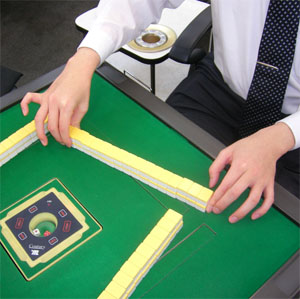
\includegraphics[width=8cm]{etiquette-1.png}
	\caption{Расположение стены}
\end{figure}

Это нужно, во-первых, чтобы тоймену было чуть проще тянуться за тайлом (а чтобы по мере разбора ему тянуться не стало сложнее, рекомендуется пододвигать свою стену время от времени), во-вторых, чтобы игроку слева было видно, есть ли в нижнем ряду тайл --- когда стена стоит параллельно его взгляду, увидеть тайл может быть сложно, в-третьих, некоторые тайлы могут быть великоваты для конкретного стола и поворотом стен игроки получают дополнительное пространство для размещения своих рук перед собой. Двигать стену рекомендуется до броска кубиков, т.к. формально бросок кубиков является началом раздачи, и случайное разрушение стены после него может наказываться штрафом. Если места хватает для всех рук и дискардов, поворачивать стены не требуется.

Перемешивание тайлов, построение стены и сортировка тайлов в своей руке (как при наборе тайлов так и во время игры) --- это действия, которые можно и нужно делать двумя руками, однако дальнейшие действия следует выполнять \textbf{одной рукой} (желательно доминантной). В случае, если игрок использует обе руки для взятий, объявлений и сбросов, судья может вынести вежливое указание играть единственной рукой. Мотивация данного ограничения исходит из того, что при игре двумя руками возрастает вероятность некорректных или даже намеренно обструктивных действий, поэтому такой практики следует избегать.

В некоторых источниках рекомендуют также делать разлом стены "лесенкой" 6-5-6, однако в других источниках, напротив, рекомендуют от этой практики отказаться:

\begin{figure}[H]
	\centering
	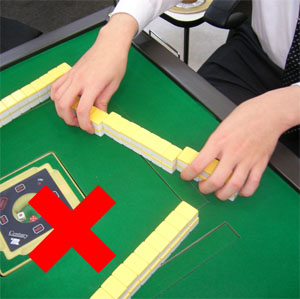
\includegraphics[width=8cm]{etiquette-2.png}
	\caption{Стена лесенкой}
\end{figure}

Считается, что такой разлом позволяет дилеру проще понять, где нужно сделать разлом, но это может не сработать, если самому сделать сдвиги неправильно. Другие аргументы за сдвиг:
\begin{itemize}
	\item Если сдвинутой стене случайно толкнуть верхний ряд --- не упадет верхний тайл на другом конце стены.
	\item Сдвиг делают, чтобы показать, что не собираются жульничать (манипуляции с такой стеной крайне затруднительны и  более очевидны).
\end{itemize} 
В итоге однозначных доводов против разлома нет, однако требовать этого от всех игроков затруднительно, так что решение о сдвиге остается за игроком.

\subsubsection{Бросок кубиков, разлом, мертвая стена}

После броска кубиков дилеру рекомендуется вслух проговорить выброшенное число, убедиться, что все игроки увидели то же самое (бывают случаи когда кому-то показалось другое число), и сразу же забрать и отложить кубики в правый угол стола. Обратите внимание, что именно кубики обозначают текущего дилера в раздаче. Индикатор раунда является индикатором первого дилера, он должен лежать у игрока, который являлся первым дилером в игре, и не должен перемещаться во время игры (только переворачиваться в начале южного раунда). 

Разлом стены может выполнить игрок, на чью стену указал бросок кубиков, также разлом может выполнить дилер одновременно со своим первым взятием. Обратите внимание, что поскольку стена всегда содержит 17 тайлов, то, когда на кубиках выброшено больше 8 --- проще отсчитать остаток с левой части стены --- например 7, когда выброшено 10, или 5, когда выброшено 12.

Игрок, в чьей стене находится изначальный индикатор доры, должен перевернуть ее, не замедляя процесса набора тайлов (если до него дошла очередь взять тайлы, то следует сначала взять их, а потом, пока тайлы берут другие игроки, открыть индикатор). Остальные действия являются опциональными: снятие первого тайла замены в мертвой стене --- действие не обязательное, но рекомендуемое:

\begin{figure}[H]
	\centering
	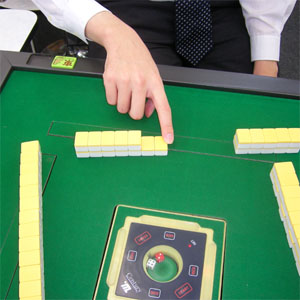
\includegraphics[width=8cm]{etiquette-3.png}
	\caption{Мертвая стена}
\end{figure}

Снятый тайл замены может остановить случайное взятие тайла не с того конца стены, т.к. мертвая стена будет визуально отличаться от живой, намекая что брать тайлы из нее не следует. 

Также рекомендуется отделить мертвую стену от живой, сделав небольшой разлом, но опять же, не замедляя процесс набора тайлов. Данное требование не является обязательным, поскольку до третьего ряда дискарда нет особого смысла беспокоиться о том, где кончается живая стена, кроме того, в случае объявления кана исходный разлом может стать неактуальным. В случае, если игрока просят отделить мертвую стену заранее, игроку следует прислушаться к просьбе.

Не следует никаким образом трогать чужие стены --- если нужно каким-либо образом подвинуть часть или всю стену, следует попросить об этом игрока, с чьей стороны находится стена. В целом, рекомендуется прикасаться к любым стенам (за исключением собственных взятий со стены) \textbf{как можно меньше}.

Недопустимо передвигать тайлы из одной стены в другую с целью полностью отделить мертвую стену --- это бессмысленная трата времени, которая к тому же иногда приводит к тому, что у игрока в стене оказывается слишком много тайлов (и такую стену банально неудобно двигать). За попытку передвигать тайлы из чужой стены в свою и наоборот может последовать вежливое указание так не делать.

\begin{figure}[H]
	\centering
	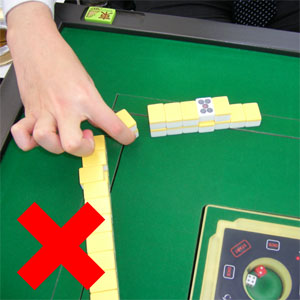
\includegraphics[width=8cm]{etiquette-4.png}
	\caption{Не трогайте чужие стены}
\end{figure}

При изначальном наборе тайлов не следует торопиться и брать тайлы не в свою очередь. Набор тайлов не в свою очередь дезориентирует игроков и приводит к гораздо большим потерям времени, чем если бы все игроки набирали тайлы последовательно.

Дилер в конце начального набора тайлов должен взять первый тайл и тайл через один от него. Брать тайлы следует осторожно, чтобы случайно не перевернуть еще не взятые тайлы, за неоднократное переворачивание тайлов из стены последует вежливое указание так не делать.

Не рекомендуется брать последние тайлы по одному, поскольку это может дезориентировать игроков (например, игрок на западе может по ошибке взять тайлы через один, как это делает дилер). Нарушение порядка разбора может привести к вежливому указанию так не делать.

\subsubsection{Набор тайлов}

Не рекомендуется набирать все тайлы рубашкой вверх и затем открывать всю руку:

\begin{figure}[H]
	\centering
	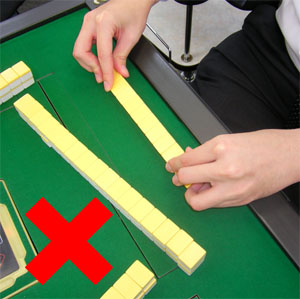
\includegraphics[width=8cm]{etiquette-5.png}
	\caption{Набор тайлов со стены}
\end{figure}

Это может привести к тому что некоторые тайлы будут вскрыты (в лучшем случае), а ближайшая стена разрушена (в худшем).

\begin{figure}[H]
	\centering
	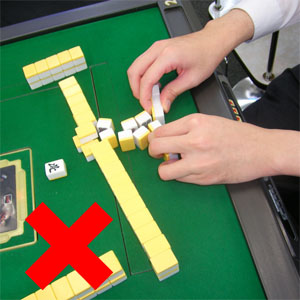
\includegraphics[width=8cm]{etiquette-6.png}
	\caption{Типичная ошибка при открытии руки}
\end{figure}

Даже если стол решит не штрафовать игрока и все согласятся на пересдачу тайлов --- это приведет к потере времени. Кроме того, открывая тайлы сразу, игрок может быстрее понять потенциалы своей руки, что сэкономит время на обдумывание первого хода. Если при этом тайлы еще и сортировать, пока другие игроки берут свои, то время экономится еще и на сортировке.

\begin{figure}[H]
	\centering
	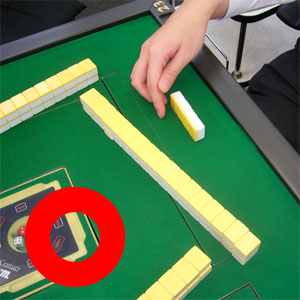
\includegraphics[width=8cm]{etiquette-7.png}
	\caption{Правильный набор руки}
\end{figure}

Отдельно стоит упомянуть, что игроки должны не забывать взять последний тайл, а дилер не должен делать первый ход, пока все игроки не набрали тайлы. Таким образом, именно дилер должен убедиться, что у всех игроков 13 тайлов в начале раздачи, и указать на это игрокам, которые забыли взять последний тайл (чаще всего забывает взять тайл игрок на севере). Нет необходимости пересчитывать тайлы в руках игроков --- достаточно взглянуть на живую стену, в ней должен быть только один свободный тайл в нижнем ряду. 

\subsection{Процесс игры}

\subsubsection{Взятие тайлов из стены}

Рекомендуется следить за тем, чтобы не показывать свои тайлы другим игрокам. Общая рекомендация --- не делать лишних движений. Например, не следует поворачивать тайл лицевой стороной к себе, пока он не окажется в зоне руки.

\begin{figure}[H]
	\centering
	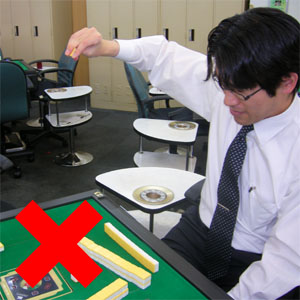
\includegraphics[width=8cm]{etiquette-8.png}
	\caption{Не делайте так при взятии}
\end{figure}

Встраивать взятый тайл в руку нельзя до момента сброса, сам же взятый тайл допустимо располагать слева или справа от руки на небольшом отдалении. Допустимо также расположить взятый тайл сверху игровой руки, поставив его на бок, однако следует избегать этого при игре наборами для автостола, поскольку магнит внутри тайла может развернуть тайл лицевой стороной к игрокам. В случае игры на камеру следует позаботиться о том, чтобы зрителям был виден тайл, который только что был взят.

Игрок вправе решать, хочет ли он сделать объявление или взять тайл со стены, только до того момента, пока он не коснулся тайла в стене. Отмена взятия со стены и взятие сета вместо этого не допускается. В случае, если другой игрок делает объявление с последнего дискарда и последовательность ходов изменяется, игрок должен вернуть взятый тайл обратно в стену (для избежания путаницы в этом случае и введено требование не встраивать тайл в руку до момента сброса).

\subsubsection{Сброс тайлов}

После первого сброса дилера, игроку на южной стороне рекомендуется убедиться, что все остальные игроки отсортировали руки и готовы продолжать игру, и только после этого делать свое взятие.

Старайтесь выполнять сброс тайла так, чтобы все игроки видели значение тайла одновременно. Некоторые игроки при сбросе тайла перекрывают видимость игроку слева, это приводит к тому, что игрок справа (чей ход следующий) видит тайл раньше игрока слева и делает свое взятие, а игрок слева, увидев тайл позже, решает объявить на нем пон или кан. Задержка приведет к тому, что игрок либо не сделает объявление, подумав что следующий тайл уже взяли (хотя технически он имеет на это право), либо к тому что пон/кан будет объявлен, но игрок справа будет знать каков следующий тайл в стене. Лучше такого избегать, в том числе, игрокам не стоит торопиться брать свой тайл после сброса слишком быстро, стоит убедиться что все игроки за столом точно видели сброс и не делают на нем объявления.

Сброс следует делать по шесть тайлов в ряд (следить за тем чтобы начинать второй ряд не раньше --- после пятого тайла, и не позже --- после седьмого):

\begin{figure}[H]
	\centering
	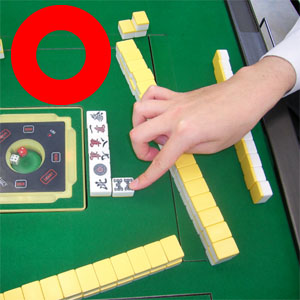
\includegraphics[width=8cm]{etiquette-9.png}
	\caption{Расположение дискарда}
\end{figure}

В случае если в третьем ряду уже лежит 6 тайлов, а тайлы в стене еще остались, следует продолжить третий ряд, а не начинать четвертый.

Нельзя забрать только что сброшенный тайл обратно в руку и сбросить другой - при нарушении может быть объявлена мертвая рука.

На сброс в среднем дается несколько секунд. Допускается размышление в течение 10-15 секунд над некоторыми сбросами, однако если игрок намеренно затягивает игру, сбрасывая каждый тайл после длительного размышления, это может быть интерпретировано как препятствование ходу игры. В этом случае следует вызвать судью и зафиксировать нарушение.

\subsection{Объявления}

В случае объявления сета, игрок обязан делать объявление громко и четко. В случае, если игроку требуется некоторое время на раздумия, игрок вправе попросить оппонентов подождать перед следующим взятием, однако не следует злоупотреблять этим правом --- если игрок слишком часто просит подождать, это может быть воспринято как затягивание игры с последующим назначением штрафа за неспортивное поведение. Не рекомендуется размышлять над взятием более 5 секунд.

\subsubsection{Объявления понов и чи}

При объявлении пона с игроков справа или напротив, игроку следует стараться сделать объявление как можно быстрее, чтобы игрок, чей ход в данный момент, не успел взять и посмотреть тайл или не объявил чи. Если очевидно, что игрок не торопится сделать взятие и раздумывает над чи --- также следует объявить пон как можно раньше, чтобы игрок не открыл тайлы в своем сете. Если игрок успел сказать "чи", допустимо сказать "пон", но следует сделать это до того как игрок открыл два своих тайла. 

Некоторые игроки практикуют "пон вредности", используя правило приоритета объявления пона над объявлением чи (ситуация: объявление "пон" непосредственно после объявления "чи", сделанное по причине того, что оппонент решает объявить чи). Данную практику мы рассматриваем как дурной тон и не рекомендуем ее использовать исходя из принципов честной игры. Однако, поскольку невозможно точно определить, является ли объявление "поном вредности" или игрок просто задумался и сделал объявление с запозданием, запретить такие объявления мы не можем и оставляем их на совести игроков. Наказаний за "пон вредности" также не предусматривается из-за сложности доказательства намерения. Игроку, который хочет объявить чи, рекомендуется выждать пару секунд, убедившись что никто не планирует объявлять пон, и только потом делать объявление. В случае объявления пона во время паузы, ситуация разрешается обычным образом в пользу объявления пона.

После объявления (которое нужно сделать достаточно громко, убедившись что все услышали и никто не пытается взять следующий тайл и продолжить игру) следует последовательно открыть два тайла из руки, потом отложить их справа от руки, далее забрать объявленный тайл, потом сформировать сет, корректно повернув взятый тайл, чтобы он указывал на игрока, с которого он был взят, отложить сет в правый угол стола, и наконец произвести сброс.

\begin{figure}[H]
	\centering
	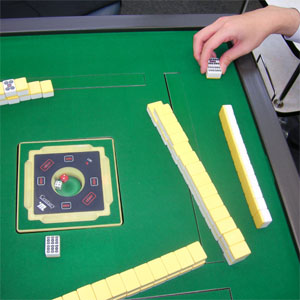
\includegraphics[width=8cm]{etiquette-10.png}
	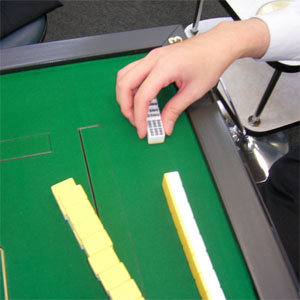
\includegraphics[width=8cm]{etiquette-11.png}
	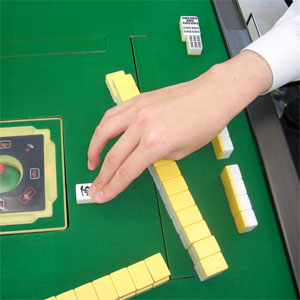
\includegraphics[width=8cm]{etiquette-12.png}
	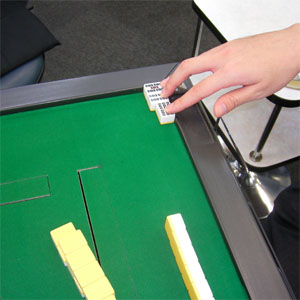
\includegraphics[width=8cm]{etiquette-13.png}
	\caption{Правильная последовательность объявление сета}
\end{figure}

Некоторые игроки, открыв два тайла, делают сброс, а затем завершают формирование сета. Следует отказаться от этой практики по двум причинам:
\begin{itemize}
	\item На вашем сбросе тоже может быть сделано объявление, и одновременно несколько тайлов будут забраны из дискардов, может произойти путаница;
	\item Можно банально забыть забрать тайл из дискарда и получить мертвую руку.
\end{itemize}

Некорректный порядок объявления может наказываться вежливым указанием (в случае повторения --- штрафом).

Некоторые игроки открывают сразу три тайла --- объявляемые и тот, который пойдет в дискард. Следует отказаться от этой практики, поскольку иногда по такому открытию неочевидно, какие именно тайлы мы объявляем, а какой готовимся сбросить (например если на сбросе 2 открыть 134). Если игрок еще не решил, что именно будет сбрасывать, следует сначала подумать, и открывать сет только после того как решение принято. Открытие трех тайлов сразу может наказываться вежливым указанием и штрафом в случае повторения.

В случае если игрок случайно открыл тайлы, которые не завершают сет, и это было быстро замечено им или указано на это другими игроками, необходимо либо открыть корректные тайлы, либо, если их в руке нет, отменить объявление. Такое поведение наказывается вежливым указанием так не делать, но может и повлечь за собой штраф в случае повторения ситуации.

В случае если никто не заметил некорректного объявления сразу, игра была продолжена, а ошибка была замечена впоследствии --- игроку назначают мертвую руку.

При объявлении нескольких сетов, можно выкладывать их в правом углу как справа налево, так и снизу вверх, но рекомендуется выкладывать именно снизу вверх, т.к. при трех и более объявлениях, когда тайлы выложены справа налево, мы будем перекрывать их видимость для других игроков при своем взятии из стены, а объявления должны быть всегда и всем видны. Не следует смешивать порядок --- например, класть второе объявление сверху над первым, а третье слева от него. Не следует класть более ранние объявления левее/выше более поздних, всегда должно быть однозначно видно, в каком порядке были сделаны объявления в раздаче.

На последнем сбросе в раздаче никакие объявления кроме объявления победы недопустимы.

\subsubsection{Объявление канов}

Открытие канов относительно похоже на объявление понов --- последовательность действий при объявлении следует соблюдать аналогичным образом. Рассмотрим отличия, характерые именно для канов.

Закрытый кан или дополнение пона до кана возможны только после взятия из стены (живой или мертвой), нельзя объявить никакой кан сразу после объявления пона/чи.

После того как игрок объявил кан и показал корректно все 4 тайла (при закрытом кане), 3 тайла при открытом кане, 1 тайл при апгрейде пона до кана (если не был объявлен рон чанкан), игрок, с чьей стороны находится новый индикатор доры, сразу переворачивает его. Игрок, объявивший кан, сформировав его в правом углу, обязательно берет тайл замены, прежде чем сделать сброс. Если игроки видят, что он готовится сбросить тайл, они должны напомнить ему о необходимости взять тайл замены. Открытые индикаторы будут применяться в том числе при победе на тайле замены.

Нужно не забывать, что после того, как игрок объявил тайл и взял тайл замены, живая стена стала на один тайл короче, т.к. в мертвой стене всегда должно быть 14 тайлов. Не рекомендуется делать каких-либо манипуляций с мертвой стеной, если до конца раздачи еще далеко --- это лишняя трата времени. Кроме того, можно запутаться и переместить в мертвую стену не тот тайл. В идеале, когда раздача будет близиться к концу, игрокам нужно прикинуть, какой тайл на данный момент будет последним, после чего можно слегка его подвинуть и указать всем условно что "последний тайл в раздаче вот этот". Если кто-то из игроков настаивает на снятии этого тайла для более простого восприятия --- игрок, в чьей стене на данный момент находится последний тайл, аккуратно его перемещает в конец живой стены, и все следят, чтобы ничего не было перепутано.

Также кратко стоит упомянуть важный момент --- кан можно объявить только если в живой стене есть хотя бы один тайл --- т.к. этот тайл нужно переместить в мертвую стену (а если тайлов в живой стене нет --- то перемещать нечего). При этом последнее взятие в игре будет из мертвой стены, в случае победы на нем будет засчитан риншан, но не хайтей (риншан и хайтей не сочетаются). При объявлении закрытого кана пятерок при игре с акадорами --- красная пятерка должна быть среди видимых, чтобы при подсчете стоимости руки ее не забыли посчитать.

\subsubsection{Объявление риичи}

Крайне важно соблюдать корректный порядок объявления: 
\begin{itemize}
	\item Громко (чтобы все услышали и обратили внимание) сказать "риичи";
	\item Сбросить тайл боком в дискард
	\item Убедиться, что на сброшенном тайле не объявлена победа
	\item Положить ставку риичи перед дискардом.
\end{itemize}

\begin{figure}[H]
	\centering
	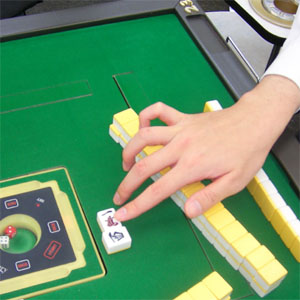
\includegraphics[width=8cm]{etiquette-14.png}
	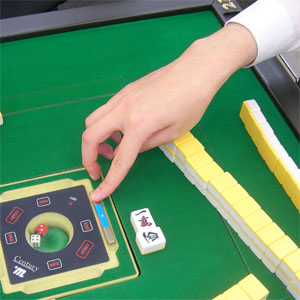
\includegraphics[width=8cm]{etiquette-15.png}
	\caption{Объявление риичи}
\end{figure}

Если тайл был взят в любой сет --- нужно не забыть повернуть свой следующий сброшенный тайл (если забыли --- сразу, как только ошибка была обнаружена, всем столом восстановить последовательность и повернуть правильный тайл). Некорректный порядок объявления риичи приводит к тому, что объявление не засчитывается. Не допускается объявлять риичи после сброса (ситуация "никому не нужно? тогда риичи"), такое риичи также не засчитывается, а за пустое объявление назначается вежливое указание так не делать, а при повторении --- штраф.

Игрок справа перед своим следующим взятием должен дождаться, пока мы выполним все действия (повернем тайл, положим палочку), и только после этого делать взятие, то же касается игроков, которые хотят на нашем тайле сделать объявление --- можно сказать "пон"/"кан", но прежде чем забирать тайл они должны дождаться, пока игрок с риичи положит палочку. При объявлении победы ждать не требуется, т.к. палочку игрок в этом случае не кладет, победу нужно объявлять сразу.

После объявления риичи игроку не следует касаться взятым из стены тайлом своей руки, чтобы избежать подозрений в изменении руки. Взятые тайлы можно смотреть, не ставя тайл в руку, также допустимо ставить рядом с рукой (справа для правшей, слева для левшей), но не касаясь ее. В случае игры на трансляции, допускается положить взятый тайл боком на руку сверху --- это позволит зрителям видеть все взятые тайлы. Не стоит класть невыигрышные тайлы лицевой стороной вверх рядом с рукой. Если тайл невыигрышный, открывать его нужно именно в дискарде, чтобы игроки не подумали, что вы объявляете победу --- за подобное расположение тайла полагается вежливое указание так не делать, а в случае повторения может быть назначен штраф.

\begin{figure}[H]
	\centering
	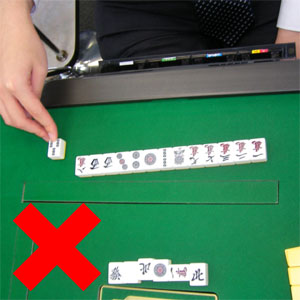
\includegraphics[width=8cm]{etiquette-16.png}
	\caption{Объявление победы при риичи}
\end{figure}

Игрок, объявивший риичи, может объявить закрытый кан, в этом случае он сначала говорит "кан", потом кладет взятый тайл лицевой стороной вверх рядом с рукой и дополняет его тремя тайлами из руки, чтобы сформировать кан.

В случае ничьей, игроки, объявившие риичи, обязательно показывают состояние своей руки, чтобы все могли убедиться, что у них есть темпай, даже если после риичи игроку по каким-то причинам была объявлена мертвая рука (например при некорректном объявлении победы). Игрок с мертвой рукой будет считаться нотен, показ руки необходим, чтобы убедиться, что риичи было корректно (в руке был темпай), а также что после риичи не было некорректных объявлений канов. В случае нарушения, игрок получает чомбо.

Риичи можно объявить только если в живой стене осталось не меньше четырех тайлов (если при отсутствии каких либо объявлений у объявляющего риичи игрока будет хотя бы одно взятие). 

Некоторые игроки приносят на турниры и на клубные игры собственные риичи-палочки, которые выглядят нестандартным образом (похоже на различные риичи-палочки на платформе MahjongSoul). Использование таких риичи-палочек не рекомендуется, однако если все игроки за столом не возражают, их использование допускается. Не следует использовать в качестве риичи-палочек посторонние предметы. Если нестандартная риичи-палочка чрезмерно отличается от стандартной (например, плохо видна на поверхности стола или может быть интерпретирована игроками как посторонний предмет), использование таких риичи-палочек также не допускается.

\subsection{Победа и ничья}

\subsubsection{Объявление победы}

При объявлении победы с дискарда следует соблюдать корректный порядок действий:

\begin{itemize}
	\item Объявить "рон" достаточно громко, чтобы все услышали, и убедиться что никто не пытается продолжить игру, взяв тайл из стены или объявив пон на том же тайле;
	\item Осторожно открыть всю руку;
	\item В случае победы с риичи --- открыть и показать всем урадоры;
	\item Перечислить все комбинации в руке, назвать общее количество дор и итоговое количество хан и фу.
\end{itemize}

В случае, если игрок забыл перевернуть индикатор урадоры, следует перевернуть его и учесть количество урадор. Если мертвая стена уже была разрушена, а результаты внесены, перерасчеты не допускаются.

Не разрешается забирать выигрышный тайл из сброса другого игрока. При нарушении может быть назначение вежливое указание (при повторном нарушении --- штраф). Обоснование заключается в том, что набросивший игрок может оспорить необходимость платить вам, т.к. в его сбросе нет вашего выигрышного тайла. Кроме того, возможны случаи, когда тайл наброшен в две и более рук. Если наброс произведен дорой, следует не забыть посчитать ее при перечислении количества дор в руке.

\begin{figure}[H]
	\centering
	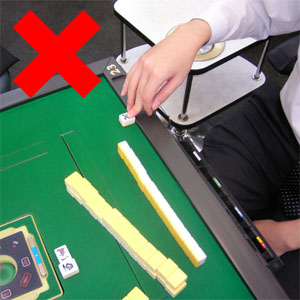
\includegraphics[width=8cm]{etiquette-17.png}
	\caption{Объявление рона}
\end{figure}

В случае выигрыша со стены также придерживаемся строгой последовательности:

\begin{itemize}
	\item Объявить "цумо" достаточно громко, чтобы все услышали, и убедиться что никто не пытается продолжить игру;
	\item Положить победный тайл сбоку от руки на некотором расстоянии. Встраивать тайл в руку не следует. Допускается сначала положить победный тайл сбоку от руки и немедленно громко объявить "цумо";
	\item Осторожно открыть всю руку;
	\item В случае победы с риичи --- открыть и показать всем урадоры;
	\item Перечислить все комбинации в руке, назвать общее количество дор и итоговое количество хан и фу.
\end{itemize}

\begin{figure}[H]
	\centering
	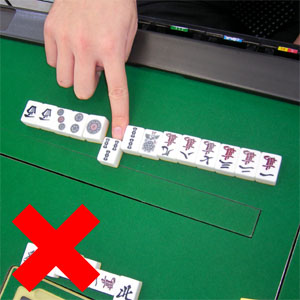
\includegraphics[width=8cm]{etiquette-18.png}
	\caption{Объявление цумо}
\end{figure}

На момент открытия рука должна быть отсортирована. В случае если игрок играет с неотсортированной рукой, допускается отсортировать руку непосредственно перед открытием. При победе следует также позаботиться о том, чтобы все ожидания в руке были очевидны, в случае сложного ожидания - рекомендуется озвучить его.

\begin{figure}[H]
	\centering
	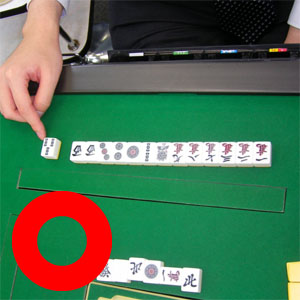
\includegraphics[width=8cm]{etiquette-19.png}
	\caption{Сортировка руки}
\end{figure}

Не следует класть победный тайл перед рукой, особенно если стена перед вами полностью разобрана --- другими игроками это может быть воспринято как сброс, на нем могут попытаться объявить победу.

\begin{figure}[H]
	\centering
	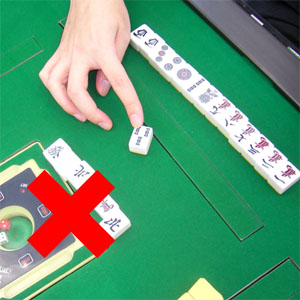
\includegraphics[width=8cm]{etiquette-20.png}
	\caption{Тайл перед рукой}
\end{figure}

В случае если игрок пытается объявить цумо положив тайл в области руки, но не сбоку от нее, ему следует вынести вежливое указание так не делать, но руку засчитать.

После объявления стоимости руки, нужно не забыть упомянуть про хонбу, если она есть, и по возможности назвать итоговую стоимость с учетом хонбы ("семь семьсот, с учетом двух хонб --- восемь триста" или "семьсот, тысяча триста, одна хонба, итого, восемьсот, тысяча четыреста").

Объявление стоимости при цумо следует начинать с меньшего значения во избежание путаницы (сравните --- "2 хан, 30 фу, пятьсот, тысяча" и "2 хан, 30 фу, тысяча пятьсот").

Объявление количества дор и якухаев рекомендуется делать максимально явным образом, например "якухай три, дора три", или "три доры, три якухая". Не рекомендуется использовать числовые обозначения для дор без упоминания слова "дора" (например, "тан-яо, три" и особенно "якухай, три" --- во избежание путаницы).

При объявлении победы, все игроки за столом имеют право проверить выигрышную руку на корректность (правильную форму, наличие яку, отсутствие фуритена). Победивший игрок не имеет права препятствовать подобным проверкам.

\subsubsection{Ничья}

При ничьей игроки показывают свой темпай. В случае если у игрока нотен, игрок должен закрыть руку или часть руки. Любое действие игрока, отличное от полного показа руки, трактуется как нотен. Рекомендуется также озвучивать состояние руки словами "темпай" и "нотен" для исключения двусмысленности.

Если игрок не объявлял риичи, он не обязан показывать руку, может объявить нотен и закрыть ее, даже если его рука открыта до одного тайла\footnote{Это может быть истиной, например при ожидании в тайл, пон которого уже открыт у игрока, но даже если это не так --- игрок в любом случае вправе закрыть руку, объявив нотен}. Объявление темпаев/нотенов следует производить поочередно, начиная с дилера (затем юг, запад, север). Открытие руки вне очереди не рекомендуется, но и не наказывается, при этом игрок имеет право не показывать состояние своей руки, пока игроки до него не покажут свое. В случае, если игрок показал темпай или нотен вне очереди, он не может поменять решение.

Дилеру может быть выгодно показать нотен, если у определенных игроков тоже нотен (например, чтобы завершить игру), но другие игроки не обязаны раскрывать ему состояние руки, пока он не объявит свое.

\subsubsection{Расчеты за победу/ничью}

После того, как победивший игрок назвал стоимость своей руки, игроки, которые делают выплаты, должны положить соответствующую сумму на стол рядом с собой. Не следует класть палочки поближе к выигравшему --- в случае цумо, когда так сделают несколько игроков, будет непонятно кто сколько положил. При расчетах следует стремиться к тому, чтобы было использовано как можно меньше палочек --- при победе в 3900 следует дать пятитысячную палочку и попросить сдачу в тысячу сто. По возможности, размен стоит производить палочками, которые уже лежат на столе, например если игрок собрал по цумо 700/1300, дилер может дать две тысячных палочки и забрать в качестве сдачи 700 очков, которые дал другой игрок, но подобные действия при расчете следует озвучивать вслух. В случае, если на столе были риичи-палочки --- победившему игроку (а в случае дабл-рона --- имеющему на них право игроку), следует сразу подвинуть их к себе, чтобы они не смешивались с очками, которыми будут производиться выплаты. Также после выплат игрокам стоит убедиться, что у них есть хотя бы одна тысячная палочка для объявления риичи, и в случае ее отсутствия попросить у других игроков размен.

\begin{figure}[H]
	\centering
	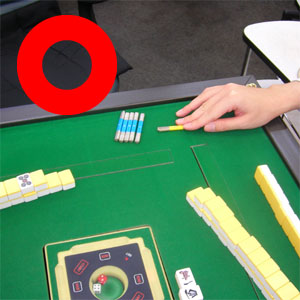
\includegraphics[width=8cm]{etiquette-21.png}
	\caption{Расчет палочками}
\end{figure}

В случае, если при объявлении риичи обнаружилось, что тысячной палочки нет --- также стоит попросить размен, желательно непосредственно перед объявлением риичи, а не в момент, когда кладется палочка, как на картинке выше.

Только после того, как очки были проверены всеми игроками и учтены, допускается перевернуть тайлы и приступить к перемешиванию тайлов, любые изменения в расчетах после этого момента производиться не должны. Если все за столом согласны, например игроки вспомнили, что забыли отметить чью-то риичи-палочку, или недосчитали дору, допустим перерасчет, но только если все игроки за столом действительно помнят, что было именно так, и не против внести изменения.

\subsection{Поведение за столом и внешний вид}

Следует обратить внимание на то, как вы сидите: не скрещивайте руки, не кладите ногу на ногу, не ставьте локти на стол и не подпирайте голову рукой:

\begin{figure}[H]
	\centering
	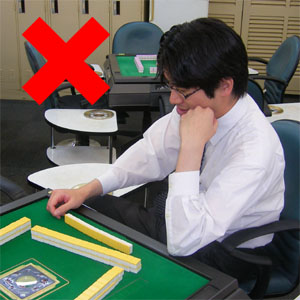
\includegraphics[width=8cm]{etiquette-22.png}
	\caption{Поза за столом}
\end{figure}

Держаться следует свободно, открыто, раскованно, нерабочую руку (для праворуких — левую и наоборот) желательно класть на колено.

\begin{figure}[H]
	\centering
	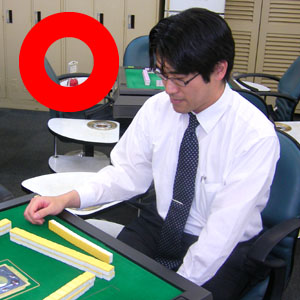
\includegraphics[width=8cm]{etiquette-23.png}
	\caption{Поза за столом}
\end{figure}

Не следует закрывать свою руку в процессе игры, в частности --- не следует закрывать руку после объявления риичи. Если рука была закрыта, другие игроки могут счесть вашу руку за часть стены и сделать взятие из нее --- в этом случае вы сами будете виноваты в том, что ваша рука признана мертвой.

\begin{figure}[H]
	\centering
	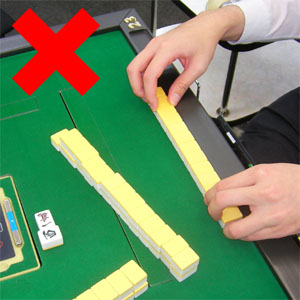
\includegraphics[width=8cm]{etiquette-24.png}
	\caption{Рука при риичи}
\end{figure}

Повторим также еще раз --- необходимо делать все объявления громко и четко, несоблюдение этого правила может быть наказано вежливым указанием или штрафом в случае повторения.

Игроки, чей внешний вид отвлекает от игры, могут быть отстранены от турнира по решению судьи. Не допускаются вызывающие костюмы, маски. Помните, что турнир - это не маскарад и не пространство для самовыражения.
	\newpage
	\section{Проведение турниров}

В данном разделе мы опишем лучшие практики организации оффлайн-турниров, которые могут быть использованы в качестве чеклиста для вашего турнира, а также быть руководством для начинающих организаторов.

Обычно подготовка турнира начинается за несколько месяцев до предполагаемой даты. В самом начале организатору предстоит определиться с датой проведения, а для этого в первую очередь необходимо договориться насчет помещения, в котором будет проводиться турнир.

\subsection{Поиск и подготовка помещения}

Обычно подготовкой турнира в городе занимаются жители этого города, поэтому мы предполагаем, что организаторы в курсе потенциальных мест для проведения турниров. Следующие варианты берутся в качестве помещения чаще всего:
\begin{itemize}
	\item Конференц-залы (отдельные или при гостиницах);
	\item Общественные места, предполагающие проведение массовых мероприятий:
	\begin{itemize}
		\item отдельные залы;
		\item залы при муниципальных заведениях;
		\item антикафе;
		\item библиотеки;
		\item заведения общественного питания;
	\end{itemize}
	\item Турниры на свежем воздухе (впрочем, обычно такие турниры делаются для весьма небольшого числа человек).
\end{itemize}

Для начала следует \textit{свериться с расписанием турниров} на ближайшие месяцы и убедиться, что ваш турнир не будет пересекаться по датам с другими, уже анонсированными турнирами. Более того, желательно выбрать дату таким образом, чтобы в диапазоне двух недель в каждую сторону не было анонсировано других турниров --- это нужно для того, чтобы дать игрокам отдохнуть, далеко не каждый готов приезжать на турнир каждые выходные.

Далее необходимо заранее \textit{договориться с местом проведения о точной дате} и о том, что вас случайным образом не попросят перенести мероприятие --- иногородним игрокам будет крайне неудобно менять билеты и бронирования в случае переноса или отмены мероприятия. Идеально, если точная дата будет известна хотя бы за 1 месяц для турниров на 20-50 человек и за 2 месяца на турниры более 50 человек.

Будьте готовы, что некоторые места могут попросить внести частичную или полную \textit{предоплату} за аренду помещения или \textit{залог}.

Помимо собственно зала, следует озаботиться отдельным \textit{помещением для зоны перекуса и зоной отдыха}, в которую могут выйти игроки после завершения игры за их столом. В качестве такой зоны может служить лобби отеля или коридор между залами. Также следует подумать про зону для курения, обычно это уличное пространство перед входом на площадку, но могут быть и другие варианты (балконы, специальные зоны для курения) --- о том, где именно можно курить, следует также явно написать в специальном регламенте турнира.

В случае, если ваш турнир предполагается проводить более одного дня, озаботьтесь договоренностью о том, что турнирное помещение будет \textit{закрыто от посторонних на вечер и ночь} --- вам будет гораздо удобнее оставить столы и наборы в помещении, чем выгружать их каждый вечер и загружать их обратно каждое утро.

Также следует заранее позаботиться о \textit{дополнительном оборудовании} --- например, проекторе и экране (если зал предусматривает их), звуковом оборудовании (микрофон, усилители, громкоговорители). Часто дополнительное оборудование можно взять в аренду в проводимом зале, либо оно может уже иметься на месте проведения. Обратите внимание, что по регламенту требуется, чтобы игроки могли видеть оставшееся до конца игры время в любой момент --- это может быть достигнуто при помощи либо использования электронного ассистента, либо проектора или экранов в зале (при их наличии).

Рекомендуется иметь хотя бы один \textit{ноутбук} для организаторских нужд, обычно его предоставляет кто-либо из организаторов. С этого ноутбука в том числе может транслироваться на проектор таймер и рассадка перед каждой игрой.

\subsection{Расписание, взносы и регламент}

Далее необходимо определиться с \textit{расписанием и регламентом} турнира. Мы предлагаем использовать текущий регламент как базу и стараться минимально отклоняться от правил и рекомендаций. Некоторые существенные отклонения могут послужить причиной невключения турнира в RR-рейтинг, в частности:
\begin{itemize}
	\item Турнир не является открытым для всех игроков. Если вы предполагаете, что участвовать смогут только игроки, прошедшие некоторый отбор, или вводите ограничения по географическому признаку, турнир будет учтен только в рейтинге CRR;
	\item Правила турнира существенно отклоняются от описанных в данном регламенте, например следующие турниры могут быть учтены только в CRR:
	\begin{itemize}
		\item Турнир по маджонгу на троих (санма);
		\item Турнир с существенными отклонениями от правил текущего регламента (в т.ч. вводящий особые правила, которые не являются общепринятыми в сообществе), далее будет приведен список допустимых вариаций;
		\item Турнир, предполагающий денежные выплаты между игроками по итогам игр.
		\item Турниры “на выживание”, длящиеся более 5 ханчанов за день;
		\item Турниры с тонпусенами вместо ханчанов;
	\end{itemize}
\end{itemize}

Также не забудьте ознакомиться со списком критериев для аккредитации турнира в RR-рейтинг, приведенным в приложении. Менее значимые вариации правил следует обсудить при подаче заявки на проведение турнира, однако мы рекомендуем избегать любых нестандартных правил.

Рассадки на турнире также следует заранее обозначить в соответствии с рекомендациями в приложении. Обратите внимание, что предполагаемую схему рассадок на турнире необходимо включить в регламент турнира, чтобы игроки заранее знали что их ждет.

\subsection{Количество игроков}

Количество игроков обычно ограничено не только снизу, но также и сверху, исходя из вместимости площадки проведения турнира. В случае, если на турнир зарегистрировалось больше игроков, чем может принять площадка, у организаторов есть два возможных варианта дальнейших действий:
\begin{itemize}
	\item Попытаться в срочном порядке найти площадку большего размера, при чем крайне желательно, чтобы площадка располагалась недалеко от исходной;
	\item Объявить явно, что игроки, зарегистрировавшиеся после определенного количества игроков в списке, проходят на турнир в порядке живой очереди и могут не попасть на турнир. В этом случае за неделю или две до турнира имеет смысл связаться лично с игроками, которые не попадают на турнир с большой вероятностью, и предупредить их об этом.
\end{itemize}

Хорошим тоном также считается предварительный опрос игроков в личном общении, если организаторам известны личные контакты игроков. В ином случае имеет смысл ориентироваться на то, внес ли игрок взнос за турнир.

\subsection{Время и расписание}

Для игровых сессий по регламенту предусматривается фиксированное время в \textbf{75 минут} основного времени. По истечении основного времени игроки должны доиграть текущую раздачу и сыграть еще одну. При составлении расписания организаторам имеет смысл рассчитывать общее время каждой игры в 90 минут, завершение оставшихся игр за 15 минут обычно не является проблемой для игроков. В случае задержек может иметь место корректирование расписания, о чем следует предупредить всех игроков.

Обычно предполагается, что турнир начинается рано утром (9 или 10 часов утра --- оптимальное время начала). Имейте в виду, что игроки будут подходить на турнир в течение какого-то времени и закладывайте это время на сбор людей. В первый день обычно предполагаются короткие вступительные мероприятия, это тоже следует учесть в расписании. В последний день турнира организаторы часто стремятся отпустить игроков пораньше, чтобы иногородние игроки успели попасть на рейсы, поэтому часто в последний день делается меньше игр, чем в предыдущие.

В зависимости от организации обеденных перерывов, игрокам нужно дать больше или меньше времени на обед, но в среднем стараются делать обеденный перерыв хотя бы на 1 час.

Пример хорошего расписания турнира:

\textbf{День 1}

\begin{itemize}
	\item \textit{9:00} --- сбор игроков
	\item \textit{9:50} --- вступительное слово организаторов
	\item \textit{10:00} --- начало первой игры
	\item \textit{11:30} --- перерыв
	\item \textit{11:45} --- начало второй игры
	\item \textit{13:15} --- перерыв на обед
	\item \textit{14:30} --- начало третьей игры
	\item \textit{16:00} --- перерыв
	\item \textit{16:15} --- начало четвертой игры
	\item \textit{17:45} --- перерыв
	\item \textit{18:00} --- начало пятой игры
	\item \textit{19:30} --- окончание первого дня турнира, консервация зала
	\item \textit{20:00 и до ночи} --- междудневные мероприятия
\end{itemize}

\textbf{День 2}

\begin{itemize}
	\item \textit{9:30} --- сбор игроков
	\item \textit{10:00} --- начало шестой игры
	\item \textit{11:30} --- перерыв
	\item \textit{11:45} --- начало седьмой игры
	\item \textit{13:15} --- перерыв на обед
	\item \textit{14:30} --- начало восьмой игры
	\item \textit{16:00} --- перерыв
	\item \textit{16:15} --- начало девятой игры
	\item \textit{17:45} --- подведение итогов, подготовка призов
	\item \textit{18:15} --- награждение призеров
	\item \textit{18:45} --- окончание второго дня турнира, уборка в зале, сбор столов и наборов
	\item \textit{19:30 и до ночи} --- послетурнирные мероприятия
\end{itemize}

Обратите внимание, что данное расписание является ориентировочным, но его необходимо опубликовать в анонсе турнира.

\textit{Задержки и отклонения от расписания} в последний день турнира являются более критичными, чем во все остальные дни, поскольку у иногородних участников с большой вероятностью уже куплены билеты на рейсы. Обратите внимание на то, что перерывы в примере длятся по 15 минут --- некоторое время от перерывов может быть использовано для компенсации задержек, очень рекомендуем предусматривать такую буферную зону.

\textbf{Размеры взносов} за турнир следует рассчитывать из следующих соображений по затратам:
\begin{itemize}
	\item Арендная плата за помещение (обычно следует ориентироваться на плату в размере не менее половины от суммы ожидаемых взносов);
	\item Арендная плата за дополнительное оборудование, если оно предполагается;
	\item Стоимость призов и приятных дополнений, если они предполагаются;
	\item Стоимость снеков, чая и прочих междуигровых перекусов;
	\item Стоимость транспортных услуг, в случае если на место нужно доставить столы;
	\item Поощрения для организаторов.
\end{itemize}

Последний пункт является опциональным, но мы рекомендуем его закладывать в стоимость, поскольку часто образуются дополнительные издержки, и в случае их отсутствия лучше распределить остатки средств по организаторам, чем распределять по организаторам же эти дополнительные издержки.

\subsection{Поиск наборов, столов, судейского состава, игроков замены}

\textbf{Поиск наборов и матов} может стать существенной проблемой для больших турниров, поэтому нужно заранее попросить игроков принести свои наборы. Учет наборов ложится на организатора, однако в любом случае лучше иметь пару запасных наборов.

Организаторы турнира также принимают на себя ответственность за возврат наборов и матов владельцам в целости. Рекомендуется вести учет --- какой набор на каком столе разложен. Хорошей практикой является вкладывание в коробку набора и в оболочку для мата номер стола, на котором этот набор используется --- это поможет при сборе наборов после турнира. Нельзя допускать, чтобы наборы перепутались (например, набор положили в коробку от другого набора; такие случаи имели место).

Организаторы также отвечают за подготовку подходящих для игры \textbf{квадратных столов и достаточного количества стульев}. Если площадка проведения может предложить квадратные столы и стулья --- поздравляем, у вас только что стало чуть меньше проблем. В случае, если квадратные столы необходимо доставить на площадку проведения, следует также заранее озаботиться о транспортировке и инструментах для сбора и разбора столов (и лучше если инструментов будет несколько, для ускорения процесса).

\textbf{Судейский состав} на турнире часто полностью или частично совпадает с организаторским, однако мы рекомендуем заранее озаботиться привлечением судей со следующим расчетом:
\begin{itemize}
	\item В случае если на турнире участвует 80 и более человек, должен быть минимум один неиграющий судья;
	\item Количество играющих судей определяется исходя из расчета одного судьи на 4-5 столов.
\end{itemize}

Начинающие судьи без судейского опыта должны при необходимости опираться на судейство других судей, нежелательно наличие в судейском составе более одного начинающего судьи.

\textbf{Игроки замены} на турнир также должны быть найдены заранее из местных игроков. Игроки замены делятся на постоянных и эпизодических. 

Постоянный игрок замены при необходимости садится за стол в первый день и играет до конца турнира. На первый день следует найти не менее трех постоянных игроков замены, чтобы можно было добить столы до кратного четырем числа игроков. В случае, если не получилось найти троих игроков, но удалось найти двух, один человек из организаторского состава должен быть готов отказаться играть в турнире в первый день, поскольку организаторы не вправе просить кого-либо из игроков сняться с турнира.

Эпизодические игроки замены должны присутствовать в качестве наблюдателей на турнире и быть готовы подменить игрока, который в какой-то момент не смог продолжать игру. Обратите внимание, что если игрок не уверен, сможет ли он присутствовать в первый день турнира, он может сыграть в турнире только в качестве эпизодического игрока замены в последующие дни. 

В общем рейтинге постоянные игроки замены учитываться не должны. Для эпизодических замен предусматривается фиксированный штраф в -30000 очков независимо от занятого места (обычно ставится -15000 штрафа и -15000 умы, в случае иной умы штраф для игроков замены должен быть оговорен отдельно в специальном регламенте турнира).

\subsection{Подготовка призов и приятных дополнений}

Часто на турнирах предусматриваются ценные призы --- они должны быть сделаны/закуплены заранее. Не следует выдавать деньги в конверте в качестве приза --- в ином случае организаторы рискуют подпасть под статью о незаконной организации и проведении азартных игр. Наиболее частые варианты призов:
\begin{itemize}
	\item Кубок и/или грамота
	\item Памятная сумка-шоппер с принтом
	\item Памятная кружка с принтом
\end{itemize}

Следует с осторожностью относиться к ценным призам, которые могут подойти не всем. Футболка с принтом скорее всего не подойдет по размеру, персональная техника может не понравиться, подарочные сертификаты в местные заведения точно не подойдут иногородним игрокам. Другими словами, основное правило --- обязательно подумать, какой приз мог бы подойти любому победителю, кем бы он ни оказался.

Иногда на турнирах также встречаются приятные дополнения для всех игроков --- например, организаторы могут выдавать каждому участнику памятные наклейки, магнитики или иные мелочи. Такие вещи также следует включить в общий бюджет турнира и озаботиться их заказом заранее.

\subsection{Освещение турнира в публичном поле и взаимодействие с игроками}

Очевидно, что чтобы на турнир пришли игроки, они должны в первую очередь об этом турнире узнать тем или иным образом. Основные способы донести анонс:
\begin{itemize}
	\item Публикация на маджонг-портале
	\item Публикация в чатах и каналах
	\item Очная реклама на других турнирах
	\item Личные приглашения
\end{itemize}

Анонс на портале должен включать \textbf{даты турнира, расписание, размеры взноса, локацию, аккредитацию (RR/CRR), контакты организаторов}. Если площадка предъявляет какие-либо требования к игрокам (например, иметь сменную обувь), или имеет какие-то особенности (например, на площадке может быть холодно и нужно запастись теплыми вещами), об этом также следует написать в анонсе на портале. Прочие публикации стоит делать более краткими, но давать ссылку на анонс на портале для уточнения деталей. В отличие от анонса на портале, анонсы в других источниках имеет смысл повторить несколько раз для привлечения как можно большего объема аудитории.

Полезно будет оставить в анонсе инструкцию и схему того, как добираться до локации от ближайших транспортных узлов (метро, остановок). Иногда может быть полезно также заснять видео прохода до площадки, если путь нетривиален.

Когда игроки пришли на турнир, их следует держать в курсе происходящего при помощи анонсов перед играми, а также посредством \textit{специально созданного чата}.

Рекомендуем создать \textbf{специальный чат турнира}, в котором будут публиковаться важные сведения как до турнира, так и в процессе и после него. Кроме того, такой чат поможет игрокам организоваться на междудневные и послетурнирные мероприятия, независимо от того, предполагается ли их централизованная организация или нет. В этом же чате можно будет решать срочные и животрепещущие вопросы с игроками.

Рекомендуется публиковать (и, при возможности, закреплять) следующую информацию в чатах:
\begin{itemize}
	\item До турнира:
	\begin{itemize}
		\item Любые непредвиденные изменения в регламенте, расписании, местоположении;
		\item Напоминания о том, что турнир близится (за месяц и за неделю до старта);
		\item (опционально) Список предлагаемых мест для обеда недалеко от места проведения;
		\item (опционально) Список гостиниц/хостелов, где можно остановиться иногородним.
	\end{itemize}
	\item Во время турнира:
	\begin{itemize}
		\item Обязательно следует закреплять время начала следующей игры. Это особенно важно в случае, если произошел сдвиг в расписании.
		\item По окончании дня, если предусмотрена централизованная организация досуговых мероприятий, закрепить место и время, в котором ждут игроков на ужин и внетурнирные игры.
	\end{itemize}
\end{itemize}

Модерация чата оставляется на усмотрение организаторов, однако общая рекомендация --- не допускать проявлений неуважения, неуместного контента, дискриминирующих и унижающих достоинство высказываний. После завершения турнира и после того, как все игроки выскажут свои впечатления и отзывы в чате, имеет смысл закрыть возможность писать сообщения в чат. 

Многие клубы имеют единственный турнирный чат, который используется периодически во время проведения турниров в городе. Другим вариантом может быть создание отдельных чатов под каждый турнир. Решение, какой именно вариант использовать, оставляется на организаторов. Пожалуйста, не удаляйте чаты после завершения турнира.

\subsection{Обеды и афтерпати}

Организаторы могут предложить централизованный обед для игроков, если площадка такое позволяет (например, при площадке есть ресторан или столовая). Договоренность с заведением питания нужно заключить \textit{заранее}, получив от заведения примерное меню и стоимость.

Для сбора сведений о тех, кто собирается обедать организованно, следует использовать интерактивные формы (Google Forms или аналогичные). В опросе нужно указать:
\begin{itemize}
	\item Ориентировочную стоимость обеда;
	\item Варианты блюд (если заведение питания предлагает такие варианты), либо обозначить конкретные блюда, которые будут на обеде, либо обозначить, что игроки смогут выбрать блюда на месте;
	\item Возможные аллергии и предпочтения (например, вегетарианская кухня).
\end{itemize}

Идеальным вариантом будет пофамильный список людей и выбранных блюд, который нужно предоставить в заведение питания за несколько дней до турнира. Имейте в виду, что чтобы накормить 50 и более человек одновременно заведению необходимо некоторое время, поэтому в договоренность с заведением обязательно следует включить точное время, к которому начнут приходить игроки на обед, чтобы заведение успело подготовить блюда к приходу игроков. Пожалуйста, убедитесь, что в заведении точно приняли к сведению, что в определенный день в определенное время ожидается большое количество посетителей --- это позволит свести к минимуму возможные опоздания после обеда.

В случае, если организаторы не планируют организовывать обеды, следует предложить игрокам как минимум несколько \textit{вариантов, где можно перекусить}. Если вокруг места проведения имеется только одно или два заведения питания, имеет смысл заранее сходить к ним и оповестить о том, что ожидается большое количество посетителей в определенные дни и в определенное время. Также в таком случае будет нелишним попытаться организовать \textit{отдельную комнату} для обеда на площадке проведения, чтобы там могли перекусить те, кто решит заказать персональную доставку блюд.

Организация междудневных досуговых активностей и афтерпати после турнира является опциональной, однако часто организаторы имеют такую возможность. При выборе помещения имеет смысл заранее поинтересоваться, кто из игроков планирует пить/есть/играть после игровых дней, и исходя из этого выбирать заведение. Желательно, чтобы в заведении имелись круглые или квадратные столы, на которых поместились бы игровые маты. Прямоугольные столы также часто приемлемы, хоть и не очень удобны.

С заведением следует договориться \textit{заранее}. Локацию и время, с которого игроков будут ожидать в заведении, следует \textit{закрепить в чате турнира}.

Поинтересуйтесь в заведении, возможно ли будет разделить счет между игроками. Некоторые заведения настаивают на том, чтобы счет был один на всех, это может быть поводом для выбора другого заведения.

\subsection{Междуигровые перекусы}

Хорошей практикой является наличие \textit{чайной зоны}, где можно налить чай и съесть пару печенек. Если при площадке проведения имеется кафе, это может быть хорошим вариантом. В ином случае организаторам придется озаботиться закупкой чая, сахара, салфеток, одноразовой посуды и воды (если воду не предоставляет площадка). Наличие чайника также будет нелишним, поскольку даже если площадка предоставляет кулер с водой, горячая вода в кулере в перерыве иссякнет очень быстро.

Доведите до сведения игроков, что \textbf{приносить еду и питье за игровые столы недопустимо} (в виде исключения можно позволить плотно закрывающиеся емкости с водой или иным напитком).

Любая алкогольная продукция во время турнира должна быть \textbf{под строгим запретом}. Игроки в состоянии алкогольного опьянения могут быть немедленно дисквалифицированы с турнира.

\subsection{Проведение турнира}

Организаторам следует позаботиться о том, чтобы к началу игр в каждый день \textit{все столы были полностью готовы} --- имели маты, наборы, индикаторы, наборы палочек в требуемом количестве. Также на каждом столе должен иметься номер стола. Рекомендуется размещать номера столов очевидным образом, чтобы игроки не искали свой стол слишком долго.

Размещение столов в зале следует делать таким образом, чтобы стулья не мешали проходу судей при необходимости. Слишком плотная посадка неудобна как для судей, так и для игроков.

Имеет смысл очертить в зале небольшую зону для складирования личных вещей (рюкзаков, сумок, верхней одежды). Это позволит игрокам иметь минимум необходимых вещей во время игры вокруг стола и расчистит проходы между столами.

После старта игр организаторы и судейский состав должны следить за порядком в зале и соблюдением относительной тишины. За слишком громкие выкрики и разговоры судьи вправе выносить вежливые указания и назначать штрафы. После завершения игры все игроки должны выйти из зала, чтобы не мешать другим --- за этим также следует следить.

Вызов судьи во время игры происходит путем поднятия руки. Не следует кричать через весь зал --- это отвлекает других игроков.

Если на турнире присутствуют наблюдатели, им \textbf{запрещено} любым образом взаимодействовать с игроками за столом (в том числе любым способом показывать любые эмоции --- противники могут использовать такую информацию для оценки силы руки игрока). В случае нарушения наблюдатель может быть удален из зала судейским составом. Некоторые игроки принципиально не допускают, чтобы кто-либо наблюдал за их рукой --- наблюдатели должны уважать это желание и переместиться в другое место по первой же просьбе игрока.

Между играми зал следует обязательно \textit{проветривать}. Как вариант, если в зале предусмотрена система кондиционирования, можно держать ее включенной во время турнира. Если турнир проводится в холодное время года и для проветривания необходимо открывать окна, следует предупредить игроков о том, чтобы они озаботились теплыми вещами.

На время подведения результатов турниров, рекомендуется \textit{удалить игроков из зала}. О точном времени начала награждения следует сообщить в турнирном чате и закрепить сообщение. После награждения может быть организовано общее фото, об этом также следует заранее сообщить игрокам (например, в устном анонсе перед началом последней игры).

\subsection{После турнира}

В течение нескольких дней после завершения турнира организаторам необходимо отправить на портал список игроков согласно занятым местам. 

Если во время турнира работал фотограф, после получения фотографий их имеет смысл опубликовать в турнирном чате.

	\newpage
	\section{Использование электронных ассистентов}

Использование электронных ассистентов в клубных играх правилами \textbf{не регламентируется}. Далее рассмотрены правила и рекомендации по использованию ассистентов в турнирных играх.

\subsection{Общие требования к турниру и к игрокам}

У каждого игрока, имеющего мобильное устройство для использования ассистента, должен быть стабильный доступ в интернет с этого устройства.

Организаторы турнира должны позаботиться о наличии стабильного WiFi-соединения с выходом в интернет. Это особенно важно в случае присутствия на турнире иностранных игроков, у которых может просто не быть местной сим-карты с доступом в интернет. Если иностранных игроков на турнире нет, наличие WiFi оставляется в качестве рекомендации.

Организаторский состав должен иметь как минимум одно общее устройство (ноутбук или компьютер) для администрирования турнира. Также с этого устройства может выводиться таймер и рассадка на проектор или экраны в зале, в случае их наличия.

Игрокам следует \textbf{заблаговременно осуществить вход в систему}. До начала турнирного дня следует проверить, что ассистент готов к использованию - проверить, что вход осуществлен и что в настройках выбран текущий турнир.

\textbf{Не рекомендуется} использовать инкогнито-режим браузера для входа в ассистент, поскольку при случайном закрытии вкладки потребуется заново входить в систему и выбирать турнир в настройках.

\subsection{Правила проведения турнира при использовании ассистента}

В общем случае использование мобильных телефонов и иных средств связи на турнирах запрещено правилами.

В случае, если на турнире предполагается использование программных средств для учета раздач и построения рейтингов, требуется придерживаться следующих правил:

\begin{itemize}
	\item Мобильным устройством допускается пользоваться \textbf{исключительно} для следующих действий:
	\begin{itemize}
		\item Внесение раздачи и предпросмотр результатов;
		\item Просмотр очков игроков за столом;
		\item Просмотр лога игры (предыдущих внесенных раздач) для контроля правильности внесенных данных.
	\end{itemize}
	\item В случае использования мобильного устройства для действий помимо описанных выше, игроки должны попросить так не делать, в случае повторения инцидента следует позвать судью для получения предупреждения и/или штрафа.
	\item При внесении раздачи игрок \textbf{обязан} показать экран предпросмотра всему столу, чтобы игроки могли увидеть перераспределение очков и в случае необходимости попросить внести коррективы.
	\item Допускается положить телефон в центр стола, чтобы игроки могли видеть свои очки и таймер в процессе раздачи.
	\item Не у всех игроков может быть подходящее мобильное устройство. В случае, если игроки просят кого-либо с мобильным устройством показать очки, игрок \textbf{не вправе} отказать.
	\item В случае, если было обнаружено, что предыдущая раздача внесена некорректно, игроки должны \textbf{позвать судью} и попросить отменить раздачу.
	\item Если вносящий игрок не умеет пользоваться ассистентом, игроки за столом обязаны помочь ему с внесением раздач и, в идеале, обучить его правильному внесению раздач.
\end{itemize}

\subsection{Игры с публикацией на стриминговых сервисах}

При использовании электронных ассистентов на крупных турнирах организаторы могут предложить организацию показательных игр с публикацией их на стриминговых сервисах (twitch).

Как правило, на стрим играет только первый стол (находящийся в топе рейтинга).

\subsubsection{Договоренности с организатором трансляции}

Организатор трансляции должен договориться с организаторами турнира включении в регламент пункта о том, что игроки первых столов соглашаются на стрим. Организатор трансляции при этом вправе выбрать, кто будет играть на камеру.

На трансляцию попадает рука только одного игрока за столом. Игрок вправе отказаться играть под камеру, если все игроки стола откажутся - организатор трансляции может предложить вывести на трансляцию второй стол из рейтинга, либо решить не транслировать стол вообще.

В случае, если предполагается транслировать руки всех игроков, требуется получить согласие каждого игрока.

\subsubsection{Дополнительные требования к играющему на трансляции}

Игрок, чья рука транслируется на стрим, должен придерживаться следующих правил:
\begin{itemize}
	\item Поскольку камера находится слева от руки игрока, недопустимо загораживать обзор своей левой рукой;
	\item Сброс тайлов желательно также осуществлять правой рукой;
	\item Руку требуется держать по центру камеры, без смещения влево или вправо. Камера должна быть настроена таким образом, чтобы центр обзора камеры совпадал с центром обзора игрока.
	\item При взятии тайла со стены, необходимо показать его на камеру. Допускается поставить тайл справа от руки, либо положить его боком сверху от руки. 
	\begin{itemize}
		\item В случае, если игра происходит на автоматическом столе, класть тайл сверху руки не рекомендуется, чтобы случайно не показать его игрокам за столом (т.к. тайлы на автостоле магнитные и положенный сверху тайл может случайно повернуться из-за этого).
	\end{itemize}
	\item Дискард следует держать в идеальном состоянии - тайлы должны быть выложены в три ряда по шесть тайлов, без промежутков между тайлами. 
	\item В случае объявления риичи, палочку-ставку следует класть непосредственно перед первым рядом дискарда.
\end{itemize}

\subsection{Форс-мажоры}

\subsubsection{Некорректная рассадка}

Перед началом игры игроки \textbf{обязаны убедиться}, что место каждого игрока соответствует тому, что отображается в ассистенте.

В случае, если была обнаружена некорректная рассадка игроков по ветрам, необходимо немедленно позвать судью и объяснить ситуацию. В случае, если сыграно немного раздач, судья может допустить последовательную отмену раздач с дальнейшим внесением их заново по принципу сохранения выигравших и проигравших. Для этого требуется сохранить куда-либо результаты всех сыгранных раздач, после чего последовательно отменить все раздачи и внести их заново. Будьте внимательны при внесении, поскольку лог раздачи содержит записи с некорректным расположением игроков.

\subsubsection{Выход из строя систем автоматизированного учета}

В случае, если продолжать турнир невозможно из-за технических неполадок, организаторам турнира следует \textbf{незамедлительно} связаться с администраторами системы учета. 

В худшем случае организаторам необходимо предоставить каждому столу ручку и лист бумаги для доигрывания игры в ручном режиме.

В случае, если сервис неработоспособен в течение длительного времени, организаторам необходимо предоставить игрокам счетные палочки и бланки для записи результатов игр. Формирование рейтинговой таблицы по итогам игр и дальнейшее проведение турнира в ручном режиме ложится на организаторов турнира.

\subsubsection{Выход из строя интернет-соединения WiFi}

Если доступ к интернету через WiFi по каким-то причинам невозможен, внесение раздач оставляется на тех игроков, которые имеют доступ в интернет через мобильную сеть. Игрок не вправе отказаться от внесения раздачи, если он единственный за столом, кто имеет доступ в интернет.

\subsubsection{Отсутствие мобильных устройств у всех игроков за столом}

В том исчезающе редком случае, если ни у одного игрока за столом нет мобильного устройства для внесения раздач, игроки вправе попросить у организаторов или у судейского состава предоставить им такое устройство. В случае, если доступного устройства нет в наличии, допускается попросить мобильное устройство у любого из столов, где таких устройств больше одного. Поиск мобильного устройства ложится на организаторский и судейский состав турнира.


	\newpage
	\section{Особенности проведения онлайн-турниров}
	
Турниры проводятся только на поддерживаемых онлайн-платформах (Mahjong soul, Tenhou net). 

\subsection{Общие положения}

Организаторы онлайн-турниров берут на себя обязательство по приведению правил турнира в соответствие с текущим регламентом. Если по какой-то причине не удается установить полное соответствие правил, либо если предполагаются отклонения от правил, организаторы обязаны сообщить об этом в сопутствующем регламенте онлайн-турнира.

В случае, если на турнир зарегистрировано некратное четырем число игроков, организаторы добавляют игроков замены в виде игровых ботов. Техническое обеспечение ложится на организаторов турнира.

Формирование рассадки для очередного тура является обязанностью организаторов турнира. Организаторы могут использовать любые технические средства автоматизации для формирования рассадок.

Игрок обязан участвовать в турнире с единственного игрового аккаунта. Каждый игровой аккаунт должен быть однозначно сопоставлен с конкретным игроком для последующего внесения в онлайн-рейтинг.

Координация турнира происходит через общий организационный чат, в который должны быть добавлены все участвующие игроки. В чате также могут присутствовать наблюдатели.

При общении в организационном чате игроки обязаны придерживаться базовых правил приличия (исключить оскорбления, переходы на личности, разжигание ненависти по любому признаку, флуд).

\subsection{Нарушения правил, специфические для онлайн-турниров}

\begin{itemize}
	\item Игрок, замеченный в одновременном использовании более чем одного аккаунта при игре в турнире, немедленно дисквалифицируется с турнира. При повторном нарушении на последующих турнирах, к игроку могут быть применены санкции вплоть до полного запрета на участие в онлайн-турнирах.
	\item Игроки, замеченные в сговоре, немедленно дисквалифицируются с турнира. При повторном нарушении на последующих турнирах, к игрокам могут быть применены санкции вплоть до полного запрета на участие в онлайн-турнирах.
	\item В случае, если турнир транслируется на стриминговом сервисе кем-либо из игроков, игрок обязан поставить задержку стрима не менее чем в 5 минут во избежание подглядывания за рукой игрока соперниками. 
	\begin{itemize}
		\item В случае, если это правило нарушено, никаких претензий относительно подглядывания другими игроками не принимается.
		\item В отдельных случаях отсутствие задержки на стриме может трактоваться как сговор (см. предыдущий пункт) со всеми соответствующими последствиями.
	\end{itemize}
	\item Организатор вправе дисквалифицировать игрока за откровенно неадекватное поведение в игре или в общем чате. В особо тяжелых случаях игрок также может быть заранее дисквалифицирован с последующих турниров. Срок дисквалификации определяется организатором турнира.
\end{itemize}

\subsection{Форс-мажоры}

В случае, если кто-либо из игроков самовольно покидает турнир до его завершения, к игроку могут быть применены санкции:

\begin{itemize}
	\item При наличии уважительной причины, вместо игрока добавляется игрок замены, получающий фиксированный штраф за каждую пропущенную игру.
	\item Организаторы имеют право сократить количество столов в случае, если суммарное количество игроков замены в турнире равно или превышает 4. В этом случае для всех игроков, которые не играют в очередном туре, применяется штраф за пропуск игры.
	\item В случае отсутствия уважительной причины, организаторы вправе дисквалифицировать игрока на определенное количество последующих онлайн-турниров, проводимых этими организаторами. Конкретное количество турниров определяется организаторами.
\end{itemize}

В случае технических неполадок на платформе, организаторы вправе досрочно завершить турнир, либо перенести оставшиеся игры на другое время. При досрочном завершении турнира, его результаты не учитываются в общем онлайн-рейтинге, турнир считается непроведенным.

Если из-за временных технических неполадок на стороне игрока он не находится в игровом лобби на момент старта его игры, игроку дается 5 минут на решение проблемы. Если неполадки не удается устранить за 5 минут, игрок заменяется на бота на время текущей игры. Рекомендуется заходить в игровое лобби заранее, чтобы было время на решение проблем в случае их возникновения.

\subsection{Технические регламенты турниров}

Техническое обеспечение разных онлайн-турниров может существенно различаться и поэтому не регламентируется в данном своде правил. Под техническим обеспечением здесь и далее подразумеваются:

\begin{itemize}
	\item Платформа для проведения игр;
	\item Организационный чат;
	\item (опционально) Средства автоматизации турнира, позволяющие провести рассадку и начать игровую сессию, например:
	\begin{itemize}
		\item Встроенные в игровую платформу средства;
		\item Бот-помощник в организационном чате;
	\end{itemize}
	\item (опционально) Рейтинговая система, например:
	\begin{itemize}
		\item Pantheon --- для полностью автоматического учета результатов;
		\item Google spreadsheets --- для ручного учета результатов;
	\end{itemize}
	\item Иные технические средства автоматизации турниров, в случае их наличия.
\end{itemize}


Организаторы турнира обязуются заранее выложить сопутствующий технический регламент, зависящий от того, какое техническое обеспечение используется на турнире. Регламент должен включать пояснения по следующим моментам:
\begin{itemize}
	\item Как корректно зарегистрироваться на турнир;
	\item Когда и где играется турнир (время с указанием часового пояса + ссылка для входа в лобби);
	\item Нужны ли дополнительные действия от игроков для учета их результатов в турнирном рейтинге, и если нужны то какие именно;
	\item Описание возможных форс-мажоров для выбранного технического обеспечения, способы их решения.
\end{itemize}

	\newpage
	\section{Регламент судейства на турнире}

Основополагающие принципы поведения на любом турнире --- \textbf{вежливость и взаимное уважение}. Однако, все же иногда могут возникать спорные ситуации, для разрешения которых необходимо привлечь независимую сторону --- турнирного судью.

Предполагается, что игроки на турнире:
\begin{itemize}
	\item Дружелюбны;
	\item Придерживаются принципов справедливой игры (fair play);
	\item Честны;
	\item Действуют в духе соревнования;
	\item Стараются действовать таким образом, чтобы неоднозначных и спорных ситуаций не могло возникнуть в принципе;
	\item Воспринимают судей как помощников на случай, если спорная ситуация все же возникла.
\end{itemize}

\subsection{Судейские роли}

Главный судья:
\begin{itemize}
	\item Отвечает за координацию работы судейской комиссии;
	\item Отвечает за обеспечение последовательности принятых решений;
	\item Является окончательной инстанцией при разногласиях внутри судейской коллегии;
	\item Осуществляет взаимодействие с организаторами турнира;
	\item Может также исполнять функции судьи.
\end{itemize}

Судья:
\begin{itemize}
	\item Отвечает за судейство на не более чем 10 столах турнира;
	\item Выносит решение максимально быстро, чтобы задержка оказалась минимальной;
	\item Не вступает в споры и не поддается на провокации;
	\item В случае несогласия игрока с решением судьи, судья вправе попросить не спорить и продолжать игру (принцип "замолчи и играй");
	\item Должен брать на заметку игроков с проблемным поведением и делиться этой информацией с другими судьями.
\end{itemize}

Пример возможного развития дискуссии:
\begin{itemize}
	\item Игрок зовет судью.
	\item Судья беседует с игроками и выносит решение.
	\item Игрок недоволен решением и высказывает жалобу судье.
	\item Судья заново обдумывает случай (может быть, сверяется с правилами), но в итоге сообщает игроку, что решение окончательное.
	\item При затруднении принятия решения, судья зовет на помощь главного судью. Главный судья выносит окончательное решение. Все возражения принимаются после игры. 
\end{itemize}

\subsection{Играющие судьи}

Допускается, что судьи могут принимать участие в турнире. На больших (80 и более человек) турнирах обязательно наличие судей, которые не принимают участие в турнире из расчета одного судьи на 10 столов, возле которых нет играющих судей.

Играющий судья может обслуживать максимум 5 соседних столов. В случае возникновения спорной ситуации за столом, где играет судья, стол обязан позвать другого судью для исключения предвзятости при вынесении решения. 

В случае, если играющий судья задерживается на вынесении решения, стол, за которым играет судья, должен получить дополнительные минуты игры. Такая ситуация в среднем рассматривается как форс-мажор (т.е. не должна происходить часто).

\subsection{Помехи при игре}

Игроки обязаны действовать разумным образом в течение всей игры, чтобы не допускать появления спорных ситуаций.

Примеры действий игроков, которые могут привести к спорным ситуациям:
\begin{itemize}
	\item Выкладывание тайлов в неположенные места (цумо близко к дискарду; объявленные сеты слева от руки)
	\item Расположение тайлов руки неположенным образом (например, закрытие руки)
	\item Слишком быстрая игра. Необходимо немного подождать перед взятием тайла со стены, чтобы все игроки могли увидеть только что сброшенный тайл и сделать соответствующие объявления.
	\item Слишком медленная игра. В случае, если игрок регулярно затягивает свои сбросы, это может трактоваться как умышленная помеха для игры. Игроки вправе вызвать судью для вынесения вежливого указания играть быстрее.
	\begin{itemize}
		\item В случае, если игроку требуется больше времени для принятия решения об объявлении, игрок вправе попросить других игроков немного подождать (но не более 10 секунд).
	\end{itemize}
	\item Шум и провокационное поведение при игре. Несмотря на то, что мы не вправе полностью запретить любое общение за столом в текущем регламенте, мы ожидаем, что игроки не будут мешать соседним столам своими разговорами. Также мы ожидаем, что игроки не будут никоим образом подначивать оппонентов на совершение тех или иных действий, вести себя вызывающе и каким-либо иным образом пытаться влиять на ход игры посредством коммуникаций.
\end{itemize}

Телефоны во время игры должны быть переведены в беззвучный режим, чтобы не мешать игрокам. Не допускается ни в какой форме голосовое общение и использование текстовых сообщений --- в случае нарушения судья может назначить штраф от 8000 до 12000 очков после умы, в случае повторного нарушения --- на усмотрение судьи. В случае, если игрок ожидает важный звонок, он должен предупредить об этом судейский состав и игроков за столом. На время звонка игроку следует выйти из зала, чтобы не мешать другим своим разговором.

Использование наушников во время игры не запрещается, при условии что игрок ясно слышит все объявления за столом. В случае возникновения спорной ситуации из-за того, что игрок не услышал объявление, игрок обязан убрать наушники до конца игры.

Игроки должны позаботиться о том, чтобы других не отвлекали в том числе посторонние запахи:
\begin{itemize}
	\item Использовать леденцы или жвачку после курения в перерыве. За столом могут быть игроки, не переносящие запах табака, уважайте их право.
	\item Любые резкие запахи, исходящие от игрока, являются веской причиной для отстранения игрока от турнира, если они не могут быть быстро устранены.
\end{itemize}

Появление игрока на турнире в состоянии алкогольного или иного опьянения недопустимо. Игроки в состоянии опьянения должны быть немедленно дисквалифицированы.

\subsubsection{Использование иных вещей игрока во время игры}

Игрок вправе принести за стол плотно закрывающуюся емкость с питьевой водой или иным безалкогольным напитком. Не допускается приносить за стол любую еду, напитки в стаканах и иных неплотно закрывающихся емкостях. В случае нарушения, судья или организатор должен немедленно унести все из вышеописанного и вежливо попросить больше так не делать. При повторном нарушении судья вправе назначить произвольный штраф.

Не допускается наличие на столе никаких вещей игроков, не относящихся к игре. Сумки следует ставить на пол рядом со стулом таким образом, чтобы они не мешали проходу судей между столами. Верхнюю одежду следует оставить в гардеробе, но также допустимо повесить на стул.

Допустимо использовать мобильный телефон в случае проведения турнира с использованием электронных средств подсчета очков. Если турнир играется на палочках, использование мобильного телефона во время игры не допускается ни в каком виде.

\subsubsection{Выход из-за стола во время игры}

Игрокам следует по возможности избегать необходимости выходить из-за стола в процессе игры. Если такая необходимость все же возникла, игроку следует вежливо попросить оппонентов подождать. В случае неоднократного повторения к такому игроку могут применены санкции на усмотрение судьи.

Оптимальным вариантом для выхода из-за стола считается время между раздачами. Игроку следует попросить других игроков замешать тайлы и построить стены во время его отсутствия с целью уменьшения задержки насколько это возможно.

Не следует выходить из-за стола без существенной причины.


\subsubsection{Передача информации во время игры}

Передача информации тем или иным образом карается штрафом на усмотрение судьи (независимо от того, насколько эта информация правдива). Примеры нарушений:
\begin{itemize}
	\item Обсуждение собственной руки вслух;
	\item Обсуждение рук и дискардов других игроков, попытки анализа дискардов вслух.
\end{itemize}

Не приветствуются, но и не наказываются попытки передачи информации, которая очевидна для всех игроков, например:
\begin{itemize}
	\item Указание на количество тайлов в руке;
	\item Показное или неконтролируемое волнение при сбросе опасного тайла.
\end{itemize}

Также не наказываются манипуляции с собственной рукой:
\begin{itemize}
	\item Карагири (сброс такого же тайла, что был взят, но из другой части руки);
	\item Умышленное отсутствие сортировки в руке;
	\begin{itemize}
		\item Заметим, что игрок, не сортирующий руку в процессе раздачи, все еще обязан ее отсортировать при победе, чтобы яку и ожидания в руке были очевидны для всех игроков;
	\end{itemize}
	\item Привычка переставлять тайлы произвольным образом, играться с тайлами также не наказывается, однако оппоненты могут попросить так не делать, если это отвлекает от игры или нервирует.
\end{itemize}

Существуют случаи передачи информации, которые не только допускаются, но и приветствуются в соответствии с духом спортивного соревнования, например:
\begin{itemize}
	\item Указание игроку на то, что он взял тайл не с той стороны стены;
	\item Указание игроку на то, что в его руке неправильное количество тайлов, что ведет к мертвой руке;
	\item Указание игроку на очевидно неправильные действия (например, вскрытие тайлов из руки, не составляющих корректный сет при объявлении, в этом случае допускается исправить сет);
	\item Озвучивание чужих и собственных сбросов в начале раздачи и в случае, если кто-либо за столом отвлекся и мог не увидеть сброс;
	\begin{itemize}
		\item Если игрок озвучивает сброс некорректно, это может быть поводом для вежливого указания так не делать;
	\end{itemize}
	\item Озвучивание открытых индикаторов дор.
\end{itemize}

\subsection{Штрафные санкции}

Предусматриваются следующие виды санкций в отношении игрока:
\begin{itemize}
	\item Вежливые указания (отсутствие штрафа):
	\begin{itemize}
		\item Применяются в случае, если требуется указать игроку на то, чтобы он сделал что-либо правильным образом (либо перестал что-то делать неправильным образом);
		\item Могут вести к ужесточению наказания в случае, если игрок не прислушался к вежливому указанию;
	\end{itemize}
	\item Мертвая рука:
	\begin{itemize}
		\item Применяется в случае, если имело место серьезное нарушение, но при этом игра все еще может продолжаться;
		\item Игрок с мертвой рукой не имеет права делать никаких объявлений (под угрозой ужесточения наказания);
	\end{itemize}
	\item Чомбо:
	\begin{itemize}
		\item Применяется в случае, если серьезное нарушение привело к тому, что раздачу продолжать невозможно;
		\item Размер штрафа чомбо --- 20000 очков после умы;
	\end{itemize}
	\item Дисциплинарный штраф:
	\begin{itemize}
		\item Применяется в случае, если игрок регулярно игнорирует вежливые указания судьи;
		\item Размер штрафа оставляется на усмотрение судьи;
		\item Штраф вычитается из итоговых очков игрока после умы;
	\end{itemize}
	\item Штрафы за опоздание:
	\begin{itemize}
		\item Применяется в случае опоздания игрока на очередную игру;
		\item Рассчитывается как 1000 очков за каждую минуту опоздания;
		\item После 10 минут опоздания вместо игрока садится игрок замены. Если игрок явился к столу позднее чем через 10 минут, он вправе продолжить игру вместо игрока замены, но при расчете итогового рейтинга после этой игры его результат будет учтен так же, как был бы учтен результат игрока замены;
	\end{itemize}
	\item Штрафы за умышленные препятствующие действия:
	\begin{itemize}
		\item Могут составлять 8000 или 12000 очков после умы в зависимости от тяжести нарушения;
	\end{itemize}
	\item Злостные и повторяющиеся случаи нарушений:
	\begin{itemize}
		\item Штраф может составлять от 12000 до 48000 очков после умы в зависимости от тяжести нарушения;
	\end{itemize}
	\item Дисквалификация игрока с турнира:
	\begin{itemize}
		\item Применяется в случае особо злостных нарушений;
		\item Также может применяться в случае неявки игрока на две игры подряд;
		\item Решение о дисквалификации игрока не только с текущего, но и с последующих турниров принимается судейской комиссией в зависимости от обстоятельств.
	\end{itemize}
\end{itemize}

\subsubsection{Случаи, допускающие самостоятельное решение спорной ситуации}

Обычно на турнире требуется звать судью для фиксации любого нарушения. Однако поскольку судей может быть ограниченное количество, некоторые ситуации могут быть разрешены игроками самостоятельно, такие ситуации обязаны отвечать следующим требованиям:
\begin{itemize}
	\item Ситуация однозначно приводит к штрафным санкциям в виде мертвой руки или чомбо;
	\item Все игроки за столом, включая игрока, попадающего под штрафные санкции, могут легко проверить, что имеет место нарушение, и согласны с тем, какие именно штрафные санкции следует применить.
\end{itemize}

Примеры разрешимых ситуаций:
\begin{itemize}
	\item У одного из игроков на руке оказалось неверное количество тайлов. Эта ситуация ведет к мертвой руке и легко проверяема всеми игроками за столом.
	\item Игрок объявил фуритен рон и открыл руку. Эта ситуация ведет к чомбо и также легко проверяема всеми игроками за столом.
\end{itemize}

Игроки обязаны позвать судью при любом из следующих условий:
\begin{itemize}
	\item У игроков есть сомнения относительно того, какие именно санкции должны быть применены;
	\item Среди игроков нет согласия относительно того, какие санкции должны быть применены;
	\item Нарушение несущественное и не приводит к штрафным санкциям, но мешает нормальной игре;
	\item Произошло злостное нарушение.
\end{itemize}

\subsection{Подсчет очков}

Игроки обязаны считать свои очки самостоятельно и по максимальной стоимости. В случае затруднений, игрокам за столом следует помочь с расчетом очков во избежание задержки.

Если игроки за столом не уверены в том, как именно рассчитать очки, они вправе позвать судью на помощь. Впрочем, такое должно происходить редко.

\subsection{Проблемное поведение игроков}

Судье не следует поддаваться ни на какие провокации со стороны игроков. Недопустимо вступать с игроками в споры и дискуссии. 

Проблемными следует считать игроков:
\begin{itemize}
	\item Игнорирующих вежливые указания судьи;
	\item Регулярно вступающих в споры относительно судейских решений;
	\item Пытающихся давить на судью или запугивать его;
	\item Регулярно зовущих судью по мелочам (особенно по таким, которые игроки могут разрешить самостоятельно);
	\item Апеллирующих к нюансам правил с целью получения выгоды (в частности, в случае просьбы игрока назначить наказание, не соответствующее нарушению).
\end{itemize}

Судейский состав должен обмениваться сведениями о том, кто из игроков является потенциально проблемным. Идеальный вариант --- ведение судейского журнала с фиксацией всех указаний и нарушений.

Наказания за нарушения для проблемных игроков следует назначать в среднем более строгие, чем всем остальным (в случаях, когда наказание оставляется на усмотрение судьи).

\subsection{Порядок вынесения решений}

Судья должен придерживаться следующего порядка выяснения обстоятельств и вынесения решения:
\begin{itemize}
	\item Посмотреть на ситуацию на столе и по возможности понять, что произошло;
	\item Поговорить со всеми игроками за столом и выслушать их аргументы; следует не допускать давления кого-либо из игроков на судью;
	\item Вынести решение и объяснить игрокам, почему это решение было вынесено. Важно, чтобы все игроки за столом понимали происходящее и никто не чувствовал, что его не выслушали.
\end{itemize}

\subsection{Обоснования для присуждения штрафов}

Основной принцип при присуждении штрафа --- чем большую помеху представляет нарушение для игрового процесса, тем строже наказание.

Размер штрафа не должен зависеть от исходных условий, например:
\begin{itemize}
	\item Если игрок нервничает или просто неловок;
	\item Если игрок неопытен и нарушает правила по незнанию;
\end{itemize}

Если игрок нарушает правила умышленно, наказание всегда должно быть строгим, однако наличие умысла должно быть однозначно доказуемым.

В следующей таблице приведены категории нарушений и соответствующие наказания. По умолчанию предполагается использовать столбец "По регламенту", однако при наличии смягчающих обстоятельств судья вправе назначить более мягкое наказание. Выяснение всех обстоятельств нарушения и принятие решения остается за судьей. 

Примечание: если в колонке "Минимальные санкции" стоит прочерк, это означает, что смягчение наказания не предусматривается.

\noindent\begin{tabularx}{\linewidth}{L{0.3\linewidth}L{0.3\linewidth}L{0.3\linewidth}}
	\caption{Обоснования штрафов} \\
	\toprule
	\textbf{Нарушение} & \textbf{По регламенту} & \textbf{Минимальные санкции} \\
	\endfirsthead
	\toprule
	\textbf{Нарушение} & \textbf{Согласно правилам} & \textbf{Минимальные санкции} \\
	\midrule
	\endhead
	\multicolumn{3}{r}{\footnotesize(Продолжение на следующей странице)}
	\endfoot
	\bottomrule
	\endlastfoot

	\multicolumn{3}{c}{\cellcolor{gray!25}Перемешивание и взятие тайлов} \\
	Ошибки при раздаче тайлов &
	Перераздача &
	- \\
	\midrule
	Недостаточное или избыточное количество тайлов на руке &
	Мертвая рука &
	- \\
	\midrule
	Некорректное взятие тайла &
	Мертвая рука &
	Вежливое указание \\
	\midrule
	Некорректный показ тайлов & 
	Мертвая рука &
	Вежливое указание \\
	\midrule
	Взятие выигрышного тайла из дискарда соперника &
	Вежливое указание &
	- \\
	\midrule
	Взятие тайла из руки соперника &
	Чомбо &
	Если соперник закрыл руку (чего делать нельзя) и из нее после этого взяли тайл, спутав со стеной, санкции остаются на усмотрение судьи. \\
	\multicolumn{3}{c}{\cellcolor{gray!25}Объявления} \\
	Ошибочное объявление открытого сета &
	Вежливое указание &
	- \\
	\midrule
	Ошибочное объявление закрытого кана &
	Вежливое указание &
	- \\
	\midrule
	Ошибочное объявление риичи &
	Мертвая рука &
	Вежливое указание \\
	\midrule
	Ошибочное объявление победы без открытия руки &
	Мертвая рука &
	- \\
	\midrule
	Ошибочное объявление победы с открытием руки &
	Чомбо & 
	- \\
	\midrule
	Любое объявление при мертвой руке & 
	Чомбо & 
	- \\
	\midrule
	Любое объявление при мертвой руке, если мертвая рука еще не объявлена &
	Мертвая рука &
	- \\
	\multicolumn{3}{c}{\cellcolor{gray!25}Открытые сеты} \\
	Невалидный открытый сет в руке &
	Мертвая рука &
	- \\
	\midrule
	Смещение сета / нарушение куикаэ &
	Мертвая рука &
	- \\
	\midrule
	Некорректное размещение тайлов в открытых сетах или в дискарде &
	Вежливое указание &
	- \\
	\multicolumn{3}{c}{\cellcolor{gray!25}Риичи} \\
	Неповернутый тайл сброса при объявлении &
	Вежливое указание &
	- \\
	\midrule
	Нотен риичи &
	Чомбо &
	- \\
	\midrule
	Открытие ожидания или всей руки при риичи &
	Мертвая рука &
	- \\
	\midrule
	Сброс тайла из руки &
	Мертвая рука; также следует проконтролировать, что был сброшен именно тот тайл, который был взят со стены. &
	- \\
	\midrule
	Объявление закрытого кана, меняющее интерпретацию структуры руки &
	Чомбо & 
	- \\
	\multicolumn{3}{c}{\cellcolor{gray!25}Неспортивное поведение} \\
	Поведение, мешающее раздаче &
	На усмотрение судьи &
	- \\
	\midrule
	Посторонние объекты на столе (не предусмотренные регламентом) &
	На усмотрение судьи & 
	- \\
	\midrule
	Передача информации (в т.ч. разглашение информации о собственной руке) &
	На усмотрение судьи &
	- \\
	\midrule
	Жульничество &
	Немедленная дисквалификация &
	- \\
	\midrule
	Подсматривание тайлов в чужой руке &
	Чомбо &
	- \\
	\multicolumn{3}{c}{\cellcolor{gray!25}Опоздания} \\
	Опоздание не более чем на 10 минут к началу игры &
	Штраф 1000 очков после умы за каждую минуту опоздания &
	- \\
	\midrule
	Опоздание более чем на 10 минут к началу игры &
	Замена игрока &
	Игрок может сесть доигрывать игру вместо замены, но в конце игры все еще получит штраф, как если бы всю игру играл игрок замены \\
	\midrule
	Пропуск ханчана &
	Замена игрока &
	- \\
	\midrule
	% TODO: check page breaks
	\linebreak\linebreak\linebreak\linebreak\linebreak & & \\
	\multicolumn{3}{c}{\cellcolor{gray!25}Вскрытие тайлов} \\
	Вскрытие 1-3 тайлов из мертвой стены &
	Мертвая рука &
	В случае случайного вскрытия единственного тайла может быть применено вежливое указание. Тайл должен быть возвращен на место. \\
	\midrule
	Вскрытие более 3 тайлов мертвой стены &
	Чомбо &
	- \\
	\midrule
	Вскрытие тайлов из живой стены &
	Чомбо &
	В случае если вскрыто незначительное количество тайлов, судья может решить, что раздача может продолжаться как есть. \\
	\midrule
	Подсматривание урадор до конца раздачи &
	Чомбо &
	- \\
	\midrule
	Показ незначительного количества тайлов из собственной руки до конца раздачи &
	Вежливое указание &
	- \\
	\midrule
	Показ значительного количества тайлов из собственной руки или всей руки до конца раздачи. Показ более половины закрытых тайлов в руке считается значительным. &
	Мертвая рука &
	- \\
	\midrule
	Вскрытие любого числа тайлов из руки соперника &
	Чомбо &
	Если соперник не объявил риичи, вскрыто не более 2 тайлов по неосторожности И если в закрытой части руки соперника более 4 тайлов, можно ограничиться вежливым указанием. \\
	\midrule
	Вскрытие некорректного индикатора доры &
	Вежливое указание; вскрытие корректного индикатора.
	
	В случае если игроки еще не видели своих рук, стол вправе устроить перераздачу. &
	- \\
	\midrule
	% TODO: check page breaks
    & & \\
	\multicolumn{3}{c}{\cellcolor{gray!25}Прочее} \\
	Закрытие руки &
	Вежливое указание &
	- \\
	\midrule
	Стол играет слишком шумно &
	На усмотрение судьи &
	Вежливое указание \\
	\midrule
	Вскрытие тайлов в стенах после объявления победы &
	Вежливое указание &
	- \\
	\midrule
	Замешивание тайлов до того, как произошел взаиморасчет &
	См. примечание ниже &
	- \\
\end{tabularx}

В случае начала замешивания тайлов до взаиморасчета, следует определить, возможно ли провести взаиморасчет на основе текущего состояния стола. Если это невозможно, игроку, замешавшему тайлы, назначается чомбо, в ином случае следует учесть столько информации, сколько возможно. В случае, если из-за замешивания дискардов не удается определить, имел ли место временный или постоянный фуритен для выигравшего игрока, замешавшему игроку также назначается чомбо.

Игроку, замешавшему тайлы мертвой стены, следует выписать штраф за неспортивное поведение. Размер штрафа оставляется на усмотрение судьи, но составляет не менее 8000 очков после умы. В случае замешивания мертвой стены до того как игроки увидели урадоры (при победе по риичи), судья имеет право решить вытянуть из замешанной части столько тайлов, сколько было урадор и учесть их в результате. 

В иных случаях, не препятствующих проведению взаиморасчета, замешивание рук и дискардов игроков, не участвующих во взаиморасчете, также не приветствуется, но на первый раз наказания не следует. Судья должен вынести вежливое указание не делать так в дальнейшем.

\subsection{Стили судейства}

Наиболее распространенные стили судейства:
\begin{itemize}
	\item "Вездесущий" судья --- следит за всеми сразу, много вмешивается, если видит нарушения;
	\item "Невидимый" судья --- приходит на помощь только в случае затруднений и нарушений.
\end{itemize}

Ожидается, что игроки сами в состоянии разрешить распространенные спорные ситуации и не будут звать судью по каждой мелочи. Таким образом, в данном регламенте мы склоняемся к невидимому стилю судейства.

Можно выделить несколько типичных ситуаций, в которых судье необходимо подойти к столу и разобраться в ситуации:
\begin{itemize}
	\item Игроки явным образом зовут судью;
	\item Игроки заметно спорят;
	\item За столом заметно существенное замешательство;
	\item За столом наблюдается препятствование игре или жульничество.
\end{itemize}

Независимо от стиля судейства, в случае если судья заметил явное нарушение, он обязан вмешаться.

Судья должен уделять внимание всем столам в своей зоне ответственности, однако он также может решить уделять больше внимания некоторым столам --- например, столам с проблемными игроками или столам, за которыми играют неопытные игроки.

Судье следует заботиться о том, чтобы не давать намеков о составе рук при выполнении судейских обязанностей.

	\newpage
	\section{Словарь терминов}

Ниже приведена таблица общеупотребительных терминов в алфавитном порядке с японскими написаниями и указанием аналогичных терминов (вариантов). Многие из этих терминов интенсивно используются в обсуждениях внутри сообщества, поэтому знание терминологии является хорошим тоном. Рекомендуем пользоваться основным вариантом каждого термина.

Список не является полным, здесь приведены только те термины, которые используются наиболее часто.

\begin{tabularx}{\linewidth}{L{0.14\linewidth}L{0.13\linewidth}L{0.1\linewidth}L{0.13\linewidth}L{0.4\linewidth}}
	\caption{Терминология} \\
	\toprule
	\textbf{Термин} & \textbf{Варианты} & \textbf{Кандзи} & \textbf{Чтение} & \textbf{Значение} \\
	\midrule
	\endfirsthead
	\toprule
	\textbf{Термин} & \textbf{Варианты} & \textbf{Кандзи} & \textbf{Чтение} & \textbf{Значение} \\
	\midrule
	\endhead
	\multicolumn{5}{r}{\footnotesize(Продолжение на следующей странице)}
	\endfoot
	\bottomrule
	\endlastfoot
	
	Агари & --- & \textnihon{和了} & \textnihon{あがり} & Объявление победы в раздаче (рон или цумо). \\
	\midrule
	Агарипай & --- & \textnihon{和了牌} & \textnihon{あがりぱい} & Выигрышный тайл (завершающий руку до победной комбинации). \\
	\midrule
	Агарияме & --- & \textnihon{和了止め} & \textnihon{あがりやめ} & Правило, согласно которому дилер имеет право завершить игру досрочно в случае лидерства после последней раздачи (оорасу). \\
	\midrule
	Адское ожидание & --- & \textnihon{地獄待ち} & \textnihon{じごくまち} & Ожидание на единственный оставшийся тайл в игре (т.е. не сброшенный в дискард и не лежащий в открытых сетах). \\
	\midrule
	Акадора & Красная дора & \textnihon{赤ドラ} & \textnihon{あかどら} & Тайл, окрашенный в красный цвет; является дорой независимо от того, что в индикаторах доры. \\
	\midrule
	Анджун & Закрытое чи & \textnihon{暗順} & \textnihon{あんじゅん} & Закрытый сет из трех последовательных тайлов мастей (закрытое шунцу) \\
	\midrule
	Анкан & Закрытый кан & \textnihon{暗槓} & \textnihon{あんかん} & Объявленный закрытый кан (закрытое канцу) \\
	\midrule
	Анко & Закрытый пон & \textnihon{暗刻} & \textnihon{あんこう} & Закрытый сет из трех одинаковых тайлов (закрытое коцу). Анкан также является анко. \\
	\midrule
	Ари & Есть & \textnihon{有り} & \textnihon{あり} & Слово, обозначающее, что какое-либо правило \textit{применяется} в данных правилах стола. Например, \textit{куитан ари} означает, что комбинация тан-яо \textit{может} быть собрана на открытой руке. \\
	\midrule
	Атама & Пара & \textnihon{頭} & \textnihon{あたま} & Пара, состоящая в выигрышной комбинации (4 сета и пара). \\
	\midrule
	Атамаханэ & --- & \textnihon{頭跳ね} & \textnihon{あたまはね} & Правило, согласно которому при объявлении победы с одного и того же сброса более чем одним игроком, приоритет имеет игрок, сидящий первым по направлению хода от игрока, сбросившего тайл. \\
	\midrule
	Атодзуке & --- & \textnihon{後付け} & \textnihon{あとづけ} & Правило, разрешающее объявлять победу в случае, если наличие яку в руке зависит от ожидания. Также используется для обозначения ситуации, когда наличие яку зависит от ожидания. \\
	\midrule
	Ветер раунда & Бакадзе & \textnihon{場風} & \textnihon{ばかぜ} & Ветер, указанный на индикаторе первого дилера на текущий момент игры. \\
	\midrule
	Бетаори & Фолд & \textnihon{ベタ降り} & \textnihon{べたおり} & Стратегия защиты, заключающаяся в сбросе заведомо безопасных тайлов (например, гэнбуцу, невозможных ожиданий) путем разрушения имеющихся форм в руке. \\
	\midrule
	Гэнбуцу & --- & \textnihon{現物} & \textnihon{げんぶつ} & Тайл, находящийся в дискарде игрока. На все гэнбуцу-тайлы у игрока фуритен. \\
	\midrule
	Даматен & --- & \textnihon{黙聴} & \textnihon{だまてん} & Скрытый темпай на закрытой руке (без объявления риичи). \\
	\midrule
	Дайминкан & --- & \textnihon{大明槓} & \textnihon{だいみんかん} & Открытый кан, объявленный при наличии в руке анко тайлов. \\
	\midrule
	Дискард & Сброс, снос & \textnihon{河} & \textnihon{かわ} & Область на столе, куда сбрасываются ненужные тайлы каждым игроком в свой ход. \\
	\midrule
	Дзянсо & --- & \textnihon{雀荘} & \textnihon{じゃんそう} & Общее название заведений для игры в маджонг в Японии. \\
	\midrule
	Дилер & Оя & \textnihon{親} & \textnihon{おや} & Раздающий игрок, игрок восточного ветра в текущей раздаче. \\
	\midrule
	Дора & --- & \textnihon{ドラ} & --- & Бонусный тайл, дающий +1 хан при победе. \\
	\midrule
	Кабэ & --- & \textnihon{壁} & \textnihon{かべ} & Техника защиты, использующая невозможность ожиданий в рянмен, пенчан и канчан при полностью видимых граничных тайлах. \\
	\midrule
	Камича & --- & \textnihon{上家} & \textnihon{かみちゃ} & Игрок, сидящий слева. \\
	\midrule
	Канцу & Кан (сет) & \textnihon{槓子} & \textnihon{かんつ} & Четыре одинаковых тайла, объявленные как кан. \\
	\midrule
	Канчан & --- & \textnihon{嵌張} & \textnihon{かんちゃん} & Внутреннее ожидание в шунцу, например 3-5 \\
	\midrule
	Каратен & --- & \textnihon{空聴} & \textnihon{からてん} & Пустое ожидание. Темпай, когда все завершающие руку тайлы уже вышли в дискард. \\
	\midrule
	Кимеучи & --- & \textnihon{決め打ち} & \textnihon{きめうち} & Способ игры, при котором игрок с начала раздачи фиксируется на сборе конкретного яку и сбрасывает все неподходящие тайлы. В подавляющем большинстве случаев кимеучи неприемлемо. \\
	\midrule
	Коцу & Пон (сет) & \textnihon{刻子} & \textnihon{こつ} & Три одинаковых тайла \\
	\midrule
	Куикаэ & --- & \textnihon{喰い替え} & \textnihon{くいかえ} & Правило, запрещающее после объявления чи или пона сброс такого же тайла, который был взят в чи/пон, а также тайла, которые мог дополнять это чи до взятия. \\
	\midrule
	Куитан & --- & \textnihon{喰い断} & \textnihon{くいたん} & Правило, разрешающее сбор тан-яо на открытой руке. \\
	\midrule
	Кюсюкюхай & --- & \textnihon{九種複数} & \textnihon{きゅうしゅ} \textnihon{きゅはい} & Пересдача при наличии в стартовой руке 9 уникальных терминальных и благородных тайлов. \\
	\midrule
	Накасудзи & --- & \textnihon{中筋} & \textnihon{なかすじ} & Судзи в середине последовательности (например, в случае 1-23-4-56-7 четверка --- накасудзи). \\
	\midrule
	Наси & Нет & \textnihon{無し} & \textnihon{なし} & Слово, обозначающее, что какое-либо правило \textit{НЕ применяется} в данных правилах стола. Противоположно "ари". \\
	\midrule
	Не-дилер & Ко & \textnihon{子} & \textnihon{こ} & Игрок, не являющийся оя (дилером) в текущей раздаче. \\
	\midrule
	Ничья & Рюкёку & \textnihon{流局} & \textnihon{りゅうきょく} & Игровая ситуация, когда никто не объявил победу до исчерпания живой стены. \\
	\midrule
	Нобетан & --- & \textnihon{延べ単} & \textnihon{のべたん} & Двойное ожидание в пару (танки), например 3-4-5-6. \\
	\midrule
	Номи & --- & \textnihon{ノミ} & --- & Буквально "только", слово, обозначающее, что кроме данного яку в руке ничего нет. Обычно применяется для яку на 1-2 хан, например "риичи номи". \\
	\midrule
	Нотен & --- & \textnihon{ノーテン} & --- & Состояние в конце раздачи, когда рука не ожидает последний тайл для завершения выигрышной комбинации. \\
	\midrule
	Объявление & Наки & \textnihon{鳴き} & \textnihon{なき} & Объявление в смысле самого процесса взятия тайла из чужого дискарда. \\
	\midrule
	Ожидание & --- & \textnihon{待ち} & \textnihon{まち} & Список тайлов, дополняющих данную руку до выигрышной. \\
	\midrule
	Ока & --- & \textnihon{オカ} & --- & Бонус победителю в игре. \\
	\midrule
	Оорасу & --- & \textnihon{オーラス} & --- & Яп. калька от "all last", последний раунд игры. \\
	\midrule
	Пайфу & Реплей & \textnihon{牌譜} & \textnihon{ぱいふ} & Подробная запись игры с расшифровками. \\
	\midrule
	Пао & --- & \textnihon{包} & \textnihon{パオ} & Ответственность за сбор последнего пона для якумана. \\
	\midrule
	Пенчан & --- & \textnihon{辺張} & \textnihon{ぺんちゃん} & Краевое ожидание в шунцу, например 1-2. \\
	\midrule
	Ренчан & --- & \textnihon{連荘} & \textnihon{れんちゃん} & Дополнительная раздача, назначаемая при победе дилера и при ничьей. \\
	\midrule
	Риншанпай & --- & \textnihon{嶺上牌} & \textnihon{りんしゃん} \textnihon{ぱい} & Тайл, который берется с мертвой стены при объявлении кана. \\
	\midrule
	Рука & Хайпай & \textnihon{配牌} & \textnihon{はいぱい} & Набор тайлов игрока. Вариант "хайпай" чаще (а в японских источниках --- всегда) используется для обозначения именно стартовой руки, для руки в целом используется термин "техай" (\textnihon{手牌}). \\
	\midrule
	Рянкан & --- & \textnihon{両嵌} & \textnihon{りゃんかん} & Двойной канчан, двойное внутреннее ожидание, например 3-5-7. \\
	\midrule
	Рянмен & --- & \textnihon{両面} & \textnihon{りゃんめん} & Двустороннее ожидание в шунцу, например 3-4. \\
	\midrule
	Рянхан-сибари & --- & \textnihon{二飜縛り} & \textnihon{りゃんはん} \textnihon{しばり} & Правило, согласно которому после 5й хонбы для победы требуется минимум 2 хан. \\
	\midrule
	Сангенпай & --- & \textnihon{三元牌} & \textnihon{さんげんぱい} & Тайлы драконов. \\
	\midrule
	Сакигири & Пуш & \textnihon{先切り} & \textnihon{さきぎり} & Потенциально опасный сброс. \\ 
	\midrule
	Сброс & --- & \textnihon{切り} & \textnihon{きり} & Выкладывание тайла в дискард в свой ход. \\ 
	\midrule
	Стена & --- & \textnihon{山} & \textnihon{やま} & Последовательность еще не взятых тайлов. \\
	\midrule
	Судзи & --- & \textnihon{筋} & \textnihon{すじ} & Дословно "интервал", тайлы мастей с промежутком в два тайла между ними (например, 1-4-7). \\
	\midrule
	Счетные палочки & Тенбо & \textnihon{点棒} & \textnihon{てんぼう} & Палочки, используемые для расчетов внутри игры и подсчета очков. \\
	\midrule
	Сянпон & --- & \textnihon{双ポン} & \textnihon{しゃんぽん} & Ожидание в два пона, например 4-4 и 9-9. \\
	\midrule
	Танки & --- & \textnihon{単騎} & \textnihon{たんき} & Ожидание в пару. \\
	\midrule
	Тацу & --- & \textnihon{塔子} & \textnihon{たーつ} & Два тайла, которым недостает третьего до сета. \\
	\midrule
	Темпай & --- & \textnihon{聴牌} & \textnihon{テンパイ} & Состояние ожидания в победу, когда до победы не хватает единственного тайла. \\
	\midrule
	Тоби & Банкрот-ство & \textnihon{トビ} & --- & Правило, согласно которому игра завершается досрочно, если кто-то из игроков уходит в минус по очкам. \\
	\midrule
	Тоймен & --- & \textnihon{対面} & \textnihon{といめん} & Игрок, сидящий напротив. \\
	\midrule
	Тойцу & Пара & \textnihon{対子} & \textnihon{といつ} & Пара одинаковых тайлов. \\
	\midrule
	Тонпуусен & --- & \textnihon{東風戦} & \textnihon{とんぷうせん} & Игра, состоящая только из восточных раундов. \\
	\midrule
	Уке-ире & --- & \textnihon{受け入れ} & \textnihon{うけいれ} & Количество и типы тайлов, которые способствуют уменьшению числа шантен в руке. \\
	\midrule
	Фуритен & --- & \textnihon{振聴} & \textnihon{ふりてん} & Состояние игрока, когда любой из его выигрышных тайлов находится в его дискарде. Игрок является фуритен даже тогда, когда в дискарде лежит тайл, который не принес бы игроку ни одного яку в руке (в случае атодзуке). \\
	\midrule
	Фурикоми & Наброс (жарг.) & \textnihon{振り込み} & \textnihon{ふりこみ} & Сброс тайла, завершающего победную руку другого игрока. \\
	\midrule
	Фуро & Открытия & \textnihon{副露} & \textnihon{ふうろ} & Вся открытая часть руки игрока. \\
	\midrule
	Хайтейпай & Последнее взятие & \textnihon{海底牌} & \textnihon{はいていぱい} & Последний тайл в живой стене. \\
	\midrule
	Ханчан & --- & \textnihon{半荘} & \textnihon{はんちゃん} & Игра, состоящая из восточных и южных раундов. \\
	\midrule
	Хаработе & & & & Форма последовательности с парным тайлом в середине, например 4556. \\
	\midrule
	Хонба & --- & \textnihon{本場} & \textnihon{ほんば} & Индикатор ренчана, обычно стоочковвая палочка. \\
	\midrule
	Хотейпай & --- & \textnihon{河底牌} & \textnihon{ほうていぱい} & Последний сброс в раздаче. \\
	\midrule
	Цумо & --- & \textnihon{自摸} & \textnihon{つも} & 1) Победа взятием со стены; 2) Тайл, взятый со стены. \\
	\midrule
	Цумогири & --- & \textnihon{自摸切り} & \textnihon{つもぎり} & Сброс тайла, только что пришедшего со стены. \\
	\midrule
	Чомбо & --- & \textnihon{冲合} & \textnihon{ちょんぼ} & Штраф за нарушения в игре, после которых игру невозможно продолжать. \\
	\midrule
	Шимоча & --- & \textnihon{下家} & \textnihon{しもちゃ} & Игрок, сидяющий справа. \\
	\midrule
	Шантен & --- & \textnihon{向聴} & \textnihon{シャンテン} & Количество тайлов, которое необходимо заменить в руке, чтобы выйти в темпай. \\
	\midrule
	Шонпай & --- & \textnihon{生牌} & \textnihon{しょんぱい} & Тайл, еще ни разу не выходивший и не лежащий в открытых сетах. \\
	\midrule
	Шоминкан & --- & \textnihon{小明槓} & \textnihon{しょうみん} \textnihon{かん} & Открытый кан, полученный докладыванием открытого пона до кана. \\
	\midrule
	Шунцу & Чи (сет) & \textnihon{順子} & \textnihon{しゅんつ} & Три тайла одной масти, образующие последовательность. \\
	\midrule
	Якитори & --- & \textnihon{焼き鳥} & \textnihon{やきとり} & 1) Правило, согласно которому игрок, который не одержал ни одной победы в игре, выплачивает штраф. 2) Состояние игрока, который не одержал ни одной победы в игре. \\
\end{tabularx}

Японское чтение цифр (ии, рян, сан, суу, уу, ро, чии, паа, чуу) не только встречается в составе названий яку, но и часто используется при обозначении тайлов, например санман --- тройка ман, уупин --- пятерка пин. Особенно полезно это знать при просмотре видео японских лиг.

Существуют некоторые варианты именования яку, которые мы, впрочем, рекомендуем не использовать по возможности:
\begin{itemize}
	\item \textit{Якухай} --- фанпай
	\item \textit{Шосанген} --- малые драконы
	\item \textit{Дайсанген} --- большие драконы
	\item \textit{Шосуши} --- малые ветра
	\item \textit{Дайсуши} --- большие ветра
	\item \textit{Цуисо} --- все благородные
	\item \textit{Тойтой} --- все поны
	\item \textit{Сан'анко} --- три закрытых пона
	\item \textit{Сууанко} --- четыре закрытых пона
	\item \textit{Санканцу} --- три кана
	\item \textit{Сууканцу} --- четыре кана
	\item \textit{Иипейко} --- два одинаковых чи
	\item \textit{Иццу} --- чистый ряд, дыхание
	\item \textit{Хон'ицу} --- грязная масть, полумасть, пол-изобилия
	\item \textit{Чин'ицу} --- чистая масть, полное изобилие
	\item \textit{Чууренпото} --- девять врат
	\item \textit{Рюисо} --- все зеленые
	\item \textit{Тан'яо} --- все простые
	\item \textit{Чинрото} --- все терминалы
	\item \textit{Чиитойцу} --- семь пар
	\item \textit{Кокуши мусо} --- 13 сирот
	\item \textit{Дабл-риичи} --- дабури
	\item \textit{Мензен цумо} --- цумо
\end{itemize}

Часто используемые сокращения:
\begin{itemize}
	\item \textit{Ментан} --- цумо + тан'яо
	\item \textit{Ментанпин} --- цумо + тан'яо + пинфу
	\item \textit{Менхон} --- закрытое хон'ицу (иногда + цумо)
	\item \textit{Менчин} --- закрытое чин'ицу (иногда + цумо)
	\item \textit{Бакахон} --- хон'ицу номи
	\item \textit{Танпин} --- тан'яо + пинфу
	\item \textit{Гоми номи} --- рука стоимостью в 300/500 (игра слов от "го" --- "пять", "ми" --- "три", "гоми" --- яп., "мусор")
\end{itemize}

Часто используемые жаргонизмы:
\begin{itemize}
	\item \textit{Дырка} --- ожидание в канчан. Иногда также так называют тацу с ожиданием в центр.
	\item \textit{Залом} --- ожидание-ловушка, например ожидание на пятерку в канчан, если двойка и восьмерка той же масти уже сброшены в дискард.
	\item \textit{Кинуть палку}, \textit{кинуть риичи} --- объявить риичи.
	\item \textit{Наброс} --- сброс тайла, на котором объявляется победа, см. фурикоми. Иногда также обозначает сброс тайла, на котором делается объявление сета.
	\item \textit{Очко} --- единица масти пин.
	\item \textit{Переехать} --- обойти по очкам либо не дать победить в раздаче, реализовать преимущество в игре.
	\item \textit{Петух} --- единица масти соу (птичка).
	\item \textit{Рофлан} --- неопытный игрок либо игрок, несерьезно относящийся к игре (пренебрежительно).
	\item \textit{Русское танки} --- ожидание в танки в форме хаработе.
	\item \textit{Русский сянпон} --- ожидание в два сянпона, каждый из которых находится в середине чи (напр., 45556 + 12223).
	\item \textit{Сгореть} --- пасть духом, разозлиться из-за неудачи в игре.
	\item \textit{Сломать руку}, \textit{сломаться} --- отказаться от сбора руки в пользу защиты, уйти в бетаори.
	\item \textit{Хиросима} --- вариант риичи-маджонга на троих. В японоязычной и англоязычной среде обычно называется "санма".
\end{itemize}
	
Обратите внимание, что данный список приведен здесь только в образовательных целях. В общем случае мы не рекомендуем использовать жаргонизмы в повседневной игре, однако знание их может помочь в разговоре с другими игроками.

	\newpage
	\section{Организационная структура комитетов}

В данном регламенте предполагается относительно большой уровень самостоятельности игроков, организаторов, судейского состава и иных лиц, принимающих решения, однако в тех случаях, когда требуется взаимодействие между различными сторонами, предлагается использовать организационные структуры и способы вынесения решений, описанные ниже.

\subsection{Оргструктуры}

Сообщество игроков состоит из, собственно, игроков, некоторые из которых наделяются рядом расширенных прав в плане принятия решений. Выделяются следующие структуры:

\begin{itemize}
	\item \textbf{Организационный комитет} --- группа, состоящая из действующих организаторов турниров в стране, на которую возлагается согласование дат турниров (с целью равномерного покрытия по месяцам и избежания пересечений по датам), а также работа с дисквалификациями.
	\item \textbf{Судейская коллегия} --- группа, состоящая из аккредитованных судей, решающая вопросы аккредитаций, отзыва аккредитаций, а также обрабатывающая жалобы и апелляции после турниров;
	\item \textbf{Комитет по правилам} --- инициативная группа, принимающая решения относительно изменений в текущем регламенте;
\end{itemize}

\subsection{Организационный комитет}

В организационный комитет входят организаторы всех турниров в стране. Организатором может стать любое инициативное лицо. 

Для координации организационного комитета используется общий чат. Начинающему организатору, который еще не участвует в комитете, следует связаться с любым действующим организатором турниров и попросить добавить его в общий чат.

Организационный комитет отвечает за согласование дат турниров таким образом, чтобы несколько турниров не выпадало на одни и те же даты. Допускается размещение на одних и тех же датах малых и средних турниров, которые предполагают участие в основном местных игроков (например, допускается поставить на одни и те же даты турниры в Иваново и во Владивостоке). Крупные турниры (с ожиданием 100 и более игроков) не должны пересекаться по датам, и кроме того интервал между двумя крупными турнирами должен составлять по меньшей мере 4 недели.

Предполагается активный обмен опытом между членами организационного комитета в области организации турниров (особенно в случае появления новых неопытных организаторов). Многие моменты касаемо организации уже описаны в текущем регламенте, однако если возникают общие проблемы, которые еще не описаны, имеет смысл внести эти проблемы и их возможные решения в раздел об организации турниров --- в этом случае организационный комитет должен сформировать предложение о правках в регламенте и предоставить его в комитет по правилам.

В случае, если в организационный комитет поступают жалобы на организацию турнира, комитет обязан рассмотреть жалобы и сформировать предложения по их решению, и довести эти предложения до всех членов комитета.

\subsubsection{Недопуск игрока на турнир}

К игроку, дисквалифицированному с одного турнира, могут быть применены жесткие санкции в виде запрета на участие в любых рейтинговых турнирах в течение определенного времени. Решение о недопуске игрока на определенный срок принимается также организационным комитетом на основании жалоб от игроков и заявлений от судейских коллегий.

Все члены организационного комитета обязуются \textbf{не принимать} на свои турниры игроков, которые не допущены до участия на момент проведения турнира.

Решение о недопуске на основании жалоб от игроков следует выносить осторожно и принимать во внимание все обстоятельства. Решение о недопуске на основании судейского заявления предполагает, что у судьи есть сильные доказательства нечестной игры, которые могут быть подтверждены как минимум одним игроком, не входящим в число аккредитованных судей.

В отдельных случаях, может возникнуть ситуация, когда игрок так или иначе совершил чистосердечное признание в том, что играл нечестно. При предъявлении соответствующих ссылок или свидетельств игроков, решение о недопуске не подлежит дальнейшему расследованию независимо от того, насколько правдивым является чистосердечное признание, т.е. шутники будут наказываться настолько же строго, насколько и нарушители.

\subsubsection{Наблюдатели}

Любой игрок, имеющий игровой опыт, может добровольно стать наблюдателем турнира и фиксировать любые нарушения со стороны судей и организаторов. По итогу турнира наблюдатель формирует отчет, который следует рассмотреть в организационном комитете и в общей коллегии судей. Наблюдатель может как принимать участие в турнире, так и быть зрителем и/или игроком замены.

Наблюдатель не обязан сообщать публично о своем статусе, однако организаторы турнира должны быть в курсе этого статуса, чтобы вовремя предоставить наблюдателю сведения о возникающих проблемах и сложностях.

Также на основании отзыва от наблюдателя судейским комитетом может быть принято решение об отзыве аккредитации судьи (см. ниже). В случае, если судья находится на испытательном сроке, присутствие наблюдателя на турнире является обязательным и судейская коллегия вправе назначить наблюдателя на турнир.

Если на турнире нет наблюдателей, отчет о проведенном турнире, возникших сложностях и проблемах ожидается от организаторов турнира.

\subsection{Судейская коллегия}

Коллегия --- инициативная группа, занимающаяся принятием решений по поводу поступивших запросов. Судейская коллегия может быть двух видов:

\begin{itemize}
	\item Общая коллегия --- включает в себя всех действующих аккредитованных судей. Занимается рассмотрением жалоб на действия конкретного судьи и имеет право отозвать аккредитацию судьи после рассмотрения жалоб (см. далее);
	\item Рабочая коллегия --- выбирается из числа действующих аккредитованных судей для рассмотрения апелляций игроков на принятые решения в ходе конкретного турнира. Рекомендуется, чтобы число судей в рабочей коллегии было нечетным для обеспечения принятия решений большинством голосов. В рабочую коллегию не должны входить судьи текущего турнира, однако имеет смысл держать их в курсе обсуждения для уточнения мотивации принятых решений.
\end{itemize}

\subsubsection{Порядок получения и обработки апелляций}

В случае, если игрок не согласен с решением судьи, либо к поведению судьи есть претензии, игрок вправе оставить апелляцию. Апелляции принимаются строго после окончания турнира.

В тексте апелляции следует максимально подробно описать спорную ситуацию, вынесенное судьей решение и причины, по которым игрок не согласен с вынесенным решением. Апелляции с недостаточно подробным описанием к рассмотрению не принимаются.

По итогу рассмотренной апелляции итоговые рейтинговые очки игрока в турнире могут быть изменены в ту или иную сторону, если судейская коллегия решит, что вынесенное судейское решение не соответствует регламенту (например, если судья выписал штраф в размере, не обоснованном регламентом). Размер компенсации или штрафа определяется судейской коллегией. Заметим, что в этом случае при изменении состава или порядка лидеров рейтинга турнира перераспределения призов не происходит, но рейтинг обновляется требуемым образом и правки учитываются в общем рейтинге страны.

Не принимаются апелляции, касающиеся турниров, для которых не применялся данный регламент. Кроме того, устанавливается срок давности в два месяца для рассмотрения апелляций, таким образом апелляции по турнирам, проведенным более чем два месяца назад, также не принимаются.

Рассмотрение апелляций может занимать некоторое время, однако рекомендуется рассмотреть все апелляции в течение месяца после подачи. 

После рассмотрения апелляции, судейская коллегия обязуется сообщить игроку, подавшему апелляцию, о принятом решении.

В случае, если апелляция касается организации турнира, судейская коллегия обязана вынести ее на обсуждение в организационный комитет с целью недопущения повторения ситуации на последующих турнирах.

\subsubsection{Получение статуса судьи}

Судьи турниров обязуются получить аккредитацию на выполнение судейских обязанностей на турнирах. Аккредитация проводится любым из уже аккредитованных судей. В процессе аккредитации судья делает презентацию по данному регламенту, а также проводит тестирование претендентов.

Тестирование проводится в форме ряда вопросов с открытыми ответами. По результатам тестирования в получении статуса судьи может быть отказано в случае, если некорректные ответы даны на более чем треть вопросов. Список действующих аккредитованных судей приводится на сайте сообщества риичи в РФ.

Судейский семинар может проводиться как в формате очной встречи, так и онлайн. В случае очной встречи, презентация проводится очно и сразу после презентации следует тестирование. В случае онлайн-аккредитации, претенденту предлагается просмотреть запись презентации и пройти онлайн-тестирование с дальнейшей беседой по удаленной связи. 

\subsubsection{Отзыв аккредитации судьи}

В случае, если к судье возникает слишком много вопросов, статус судьи может быть отозван общей судейской коллегией. Порядок рассмотрения запросов на отзыв статуса судьи:

\begin{itemize}
	\item Получение и фиксирование жалоб на конкретного судью.
	\item Вынесение жалоб на рассмотрение судейской коллегии. Коллегия выносит решение о том, насколько критичны и насколько обоснованы поступившие жалобы. На данном этапе процесс может быть прекращен в случае недостаточной обоснованности или критичности жалоб.
	\item Оповещение судьи о том, какие действия ему следует предпринять, чтобы исправить проблемы, на которые указали игроки.
	\item В случае, если судья продолжает допускать грубые ошибки при судействе, наблюдатель ставит на обсуждение вопрос об отзыве судейской аккредитации.
	\item Судейская коллегия рассматривает отзыв наблюдателя и принимает решение об отзыве судейской аккредитации.
\end{itemize}

\subsection{Комитет по правилам}

Данный комитет формируется из заинтересованных лиц, имеющих конкретные предложения по поводу модификации текущего регламента.

В случае, если требуются изменения в регламенте, определяется следующий порядок внесения изменений:
\begin{itemize}
	\item Определение конкретных пунктов, в которых требуются правки ("что правим") и определение конкретных предложений ("как правим");
	\item Предварительный сбор мнений с игроков. Для рассмотрения предложения требуется, чтобы не менее 10 игроков поддержали предлагаемые изменения.
	\item Вынесение предложения на обсуждение в сообществе. Круг заинтересованных лиц не регламентируется и принимаются доводы от любого игрока. В интересах комитета по правилам согласовать изменения с максимально возможным количеством заинтересованных лиц в сообществе, чтобы избежать недопонимания и обеспечить легитимность изменений.
	\item Внесение изменений в регламент и дальнейшая его публикация в соответствии с графиком.
\end{itemize}

Публикация регламента осуществляется \textbf{раз в полгода} и включает все изменения, внесенные за последние полгода. В случае отсутствия изменений, публикация может быть отложена до следующего периода. До публикации изменений следует пользоваться текущей версией регламента, однако допускается точечное внесение грядущих изменений в регламенты турниров организаторами.

Каждое изменение в регламенте должно сопровождаться кратким списком того, что именно было изменено, чтобы людям не приходилось перечитывать регламент полностью каждый раз. В списке изменений следует указывать конкретный номер пункта регламента, который был изменен, а также приводить описание изменения. Список изменений следует приводить в приложении к текущему регламенту.

В случае, если организуется новый комитет по правилам, настоятельно рекомендуется включать в его состав людей, принимавших ключевые решения при подготовке предыдущих версий регламента. Эти люди смогут объяснить причины появления тех или иных пунктов в текущем регламенте и таким образом избежать повторных длительных обсуждений.

	\newpage
	\section{Заключение}

В данном регламенте мы постарались максимально охватить как все вопросы, регулярно возникающие у начинающих игроков, так и нюансы в процессе проведения турниров и клубных игр. В случае возникновения каких-либо вопросов или уточнений, просим обращаться в рабочую группу по правилам, все вопросы обязательно будут рассмотрены и при необходимости будут внесены правки.

Редакции правил предполагается обновлять раз в год. В случае отсутствия существенных правок, выпуск новой редакции может быть отменен. При проведении турниров просим указывать версию (год выпуска) регламента правил, которые вы собираетесь использовать на турнире. Ожидается, что все судьи турнира ориентируются в регламенте и следят за актуальностью своих знаний. Рабочая группа обязуется обеспечить максимальное публичное распространение новых редакций по мере их выхода.

Спасибо за внимание и ждем вас на турнирах!

	
\end{document}
